% !TEX root = main.tex
\section{Time-dependent amplitude fit}
\label{sec:fullFit}

The signal PDF used for the full time-dependent fit is defined as
\begin{equation}
\label{eq:ampPDF_full}
\mathcal{P}(\phsPoint, t \vert\delta t, q_{OS}, \eta_{OS}, q_{SS}, \eta_{SS}) \propto \left[ p(\phsPoint, t^{'} \vert q_{OS}, \eta_{OS}, q_{SS}, \eta_{SS})  \otimes \mathcal{R}(t - t^{'},\delta t) \right] \cdot \epsilon(t)
\end{equation}
where $p(\phsPoint, t \vert q_{OS}, \eta_{OS}, q_{SS}, \eta_{SS})$ is given the differential decay rate in Equation \ref{eq:PDF_full2} taking the tagging dilution into account.
The phase space efficiency $\epsilon(\phsPoint)$ is only included in the normalization of $\mathcal{P}(\phsPoint, t \vert\delta t, q_{OS}, \eta_{OS}, q_{SS}, \eta_{SS})$
as discussed in Sec~\ref{sec:phasespaceAcceptance}. 
The model selection of the amplitude components is described in the following Section.
The remaining fitting strategy is exactly the same as for the decay-time fits, see Sec.~\ref{sec:timeFit}.

\subsection{Signal Model Construction}
\label{sec:LASSO}

The light meson spectrum comprises multiple resonances which are expected to contribute to $B_s \to D_s K \pi \pi$  decays as intermediate states. 
Apart from clear contributions coming from resonances such as $K_{1}(1270)$, $K_{1}(1400)$, $\rho(770)$ and $K^*(892)^0$, 
the remaining structure is impossible to infer due to
the cornucopia of broad, overlapping and interfering resonances 
within the phase space boundary.
We follow the \textsf{LASSO} \cite{Tibshirani94regressionshrinkage,Guegan:2015mea} approach 
to limit the model complexity in two steps.

First, we fit the time-integrated and flavour averaged phase-space distribution of $B_s \to D_s K \pi \pi$  decays.
In this case, a single total amplitude can be used:
\begin{equation}
\mathcal A_f^{eff}(\phsPoint) = \sum_i a^{eff}_i  A_i(\phsPoint)
\end{equation}
which effectively describes the incoherent superposition of the $b\to c$ and $b\to u$ amplitudes:
\begin{equation}
	\mathcal  \vert A_f^{eff}(\phsPoint)  \vert^{2} = \mathcal  \vert A_f^c(\phsPoint)  \vert^{2} +  \mathcal  \vert A_f^u(\phsPoint)   \vert^{2}   .
\end{equation}
This significantly simplifies the fitting procedure and allows us 
to include the whole pool of considered intermediate state amplitudes $A_i$ which can be found in Appendix \ref{a:decays}.
% allows us to identify the contributing resonances 
%To build the amplitude model, one could successively add amplitudes on top of one another until a reasonable agreement between data and fit was achieved.
%However, this step-wise approach is not particularly suitable for amplitude analyses as discussed in Ref.~\cite{Guegan:2015mea}.
%Instead, we include the whole pool of amplitudes in the first instance and use the 
%Least Absolute Shrinkage and Selection Operator~\cite{Tibshirani94regressionshrinkage,Guegan:2015mea} (LASSO) approach to limit the model complexity.
The LASSO penalty term added to the likelihood function
\begin{equation}
	-2 \, \log \mathcal L \to -2 \, \log \mathcal L + \lambda \, \sum_{i} \sqrt{ \int \vert a^{eff}_i  A_i(\phsPoint) \vert^{2} \, \text{d}\Phi_{4}  },
\end{equation}
shrinks the amplitude coefficients towards zero.
The amount of shrinkage is controlled by the parameter $\lambda$, to be tuned on data.
Higher values for $\lambda$ encourage sparse models, \ie models with only a few non-zero amplitude coefficients.
The optimal value for $\lambda$ is found by minimizing the Bayesian information criteria~\cite{BIC} (BIC),
\begin{equation}
	\text{BIC}(\lambda) = - 2 \, \log \mathcal L + r  \, \log N_{\rm Sig},
\end{equation}
where $N_{\rm Sig}$ is the number of signal events and $r$ is the number of amplitudes with a decay fraction above 
a certain threshold.
The fit fractions are defined as
\begin{equation}
\label{eq:DefineFitFractions}
	F_{i} \equiv \frac{\int \left\vert   a^{eff}_{i} \, A_{i}(\phsPoint) \right\vert^{2} \, \text{d}\Phi_{4} }
	{\int \left\vert  \mathcal A_f^{eff}(\phsPoint) \right\vert^{2} \, \text{d}\Phi_{4}}, 
\end{equation}
and are a measure of the relative strength between the different transitions. 
%In this way, the optimal $\lambda$ balances
%the fit quality ($- 2 \, \log  \mathcal L$) against the model complexity.
%The LASSO penalty term is only used to select the model. 
%Afterwards, this term must be discarded in the final amplitude fit with the selected model, otherwise the parameter uncertainties would be biased. 
%The set of amplitudes is selected using the optimal value of $\lambda=28$, and is henceforth called the LASSO model; 
Figure \ref{fig:BIC}(left) shows the distribution of BIC values obtained by scanning over $\lambda$
where we choose the decay fraction threshold to be $0.5 \%$.
At the optimal value of $\lambda=50$, the set of amplitudes with a decay fraction above the threshold 
are considered further for step two of the model selection.
The selected amplitudes and their fractions are summarized in Table \ref{tab:lassoFit}.
The fit projections are shown in Fig.~\ref{fig:lassoFit}.

In Stage 2, the LASSO procedure is again performed by fitting the full time-dependent amplitude PDF.
The components selected by Stage 1 are included for both $b\to c$ and $b\to u$ transitions and the likelihood is extended as follows:
\begin{equation}
	-2 \, \log \mathcal L \to -2 \, \log \mathcal L + \lambda \, \sum_{i} \sqrt{ \int \vert a^{c}_i  A_i(\phsPoint) \vert^{2} \, \text{d}\Phi_{4}  }  + \lambda \, \sum_{i} \sqrt{ \int \vert a^{u}_i  A_i(\phsPoint) \vert^{2} \, \text{d}\Phi_{4}  } 
\end{equation}
Figure \ref{fig:BIC}(right) shows a plot of the complexity factor
$\lambda$, against the resulting BIC values. 
The final set of $b\to c$ and $b\to u$ amplitudes is selected using the optimal value of $\lambda=28$, and is henceforth called the LASSO model.

\begin{figure}[b]
  \centering
  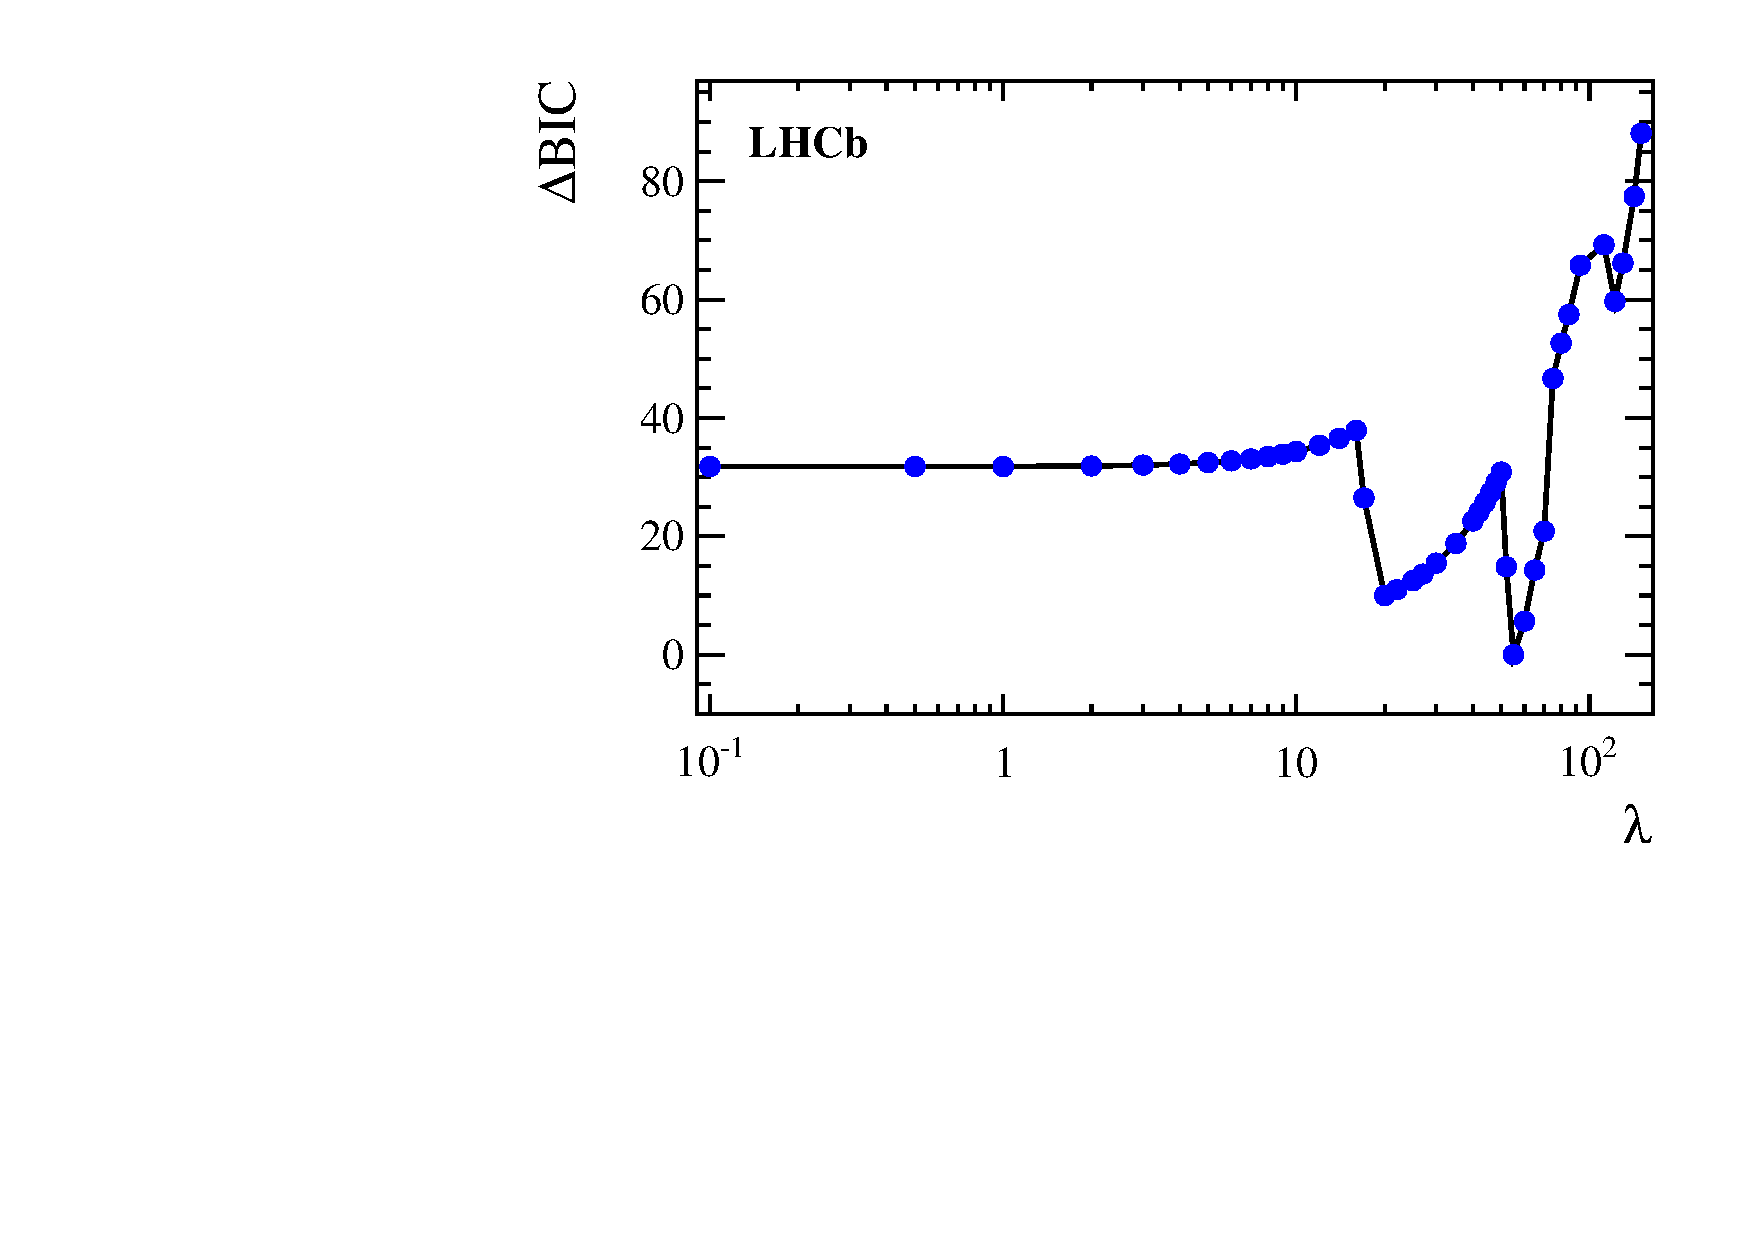
\includegraphics[width=0.45\textwidth, height=!]{figs/lassoFit/Lasso_BIC.pdf} 
  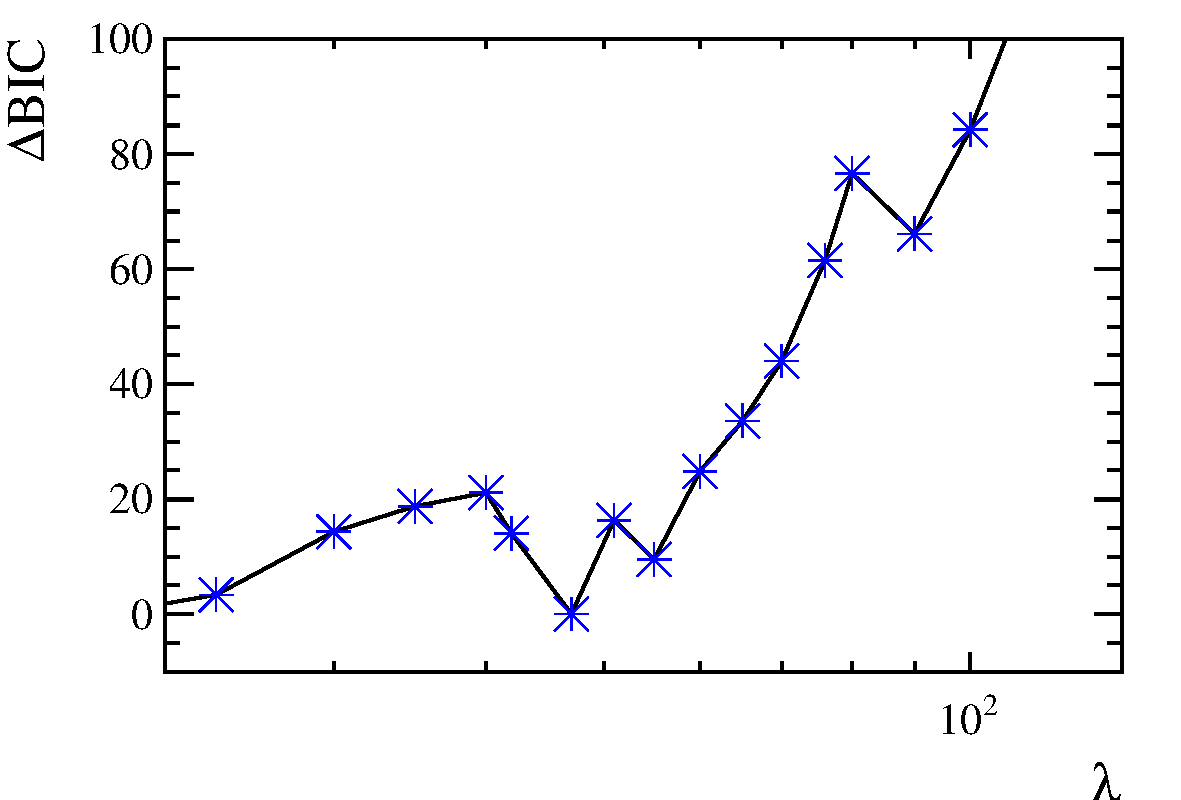
\includegraphics[width=0.45\linewidth, height=!]{figs/fullFit/ReLasso_BIC.pdf}
  \caption{Difference in the BIC value from its minimum as function of the LASSO parameter $\lambda$ for step 1 (left) and step 2 (right) of the model selection.}
  \label{fig:BIC}
\end{figure}

\begin{table}[h]
\centering
\caption{
\small Fit fractions of the amplitudes selected by Stage 1 of the model selection procedure.
}
\begin{tabular}{l r}
\hline
\hline
Decay channel & Fraction [$\%$] \\
\hline
$B_s \to K(1)(1270)^+( \to K^*(892)^0( \to K^+ \, \pi^-) \, \pi^+) \, D_s^-$ & 7.41 $\pm$ 0.98 \\
$B_s \to K(1)(1400)^+( \to K^*(892)^0( \to K^+ \, \pi^-) \, \pi^+) \, D_s^-$ & 36.18 $\pm$ 2.16 \\
$B_s \to K(1460)^+( \to K^*(892)^0( \to K^+ \, \pi^-) \, \pi^+) \, D_s^-$ & 4.12 $\pm$ 0.47 \\
$B_s \to K^*(1410)^+( \to K^*(892)^0( \to K^+ \, \pi^-) \, \pi^+) \, D_s^-$ & 15.03 $\pm$ 0.75 \\
$B_s \to ( D_s^- \, \pi^+)_{P} \, K^*(892)^0( \to K^+ \, \pi^-)$ & 7.47 $\pm$ 0.82 \\
$B_s \to K^*(1410)^+( \to \rho(770)^0( \to \pi^+ \, \pi^-) \, K^+) \, D_s^-$ & 5.39 $\pm$ 0.47 \\
$B_s \to ( D_s^- \, K^+)_{P} \, \rho(770)^0( \to \pi^+ \, \pi^-)$ & 1.51 $\pm$ 0.27 \\
$B_s \to K(1)(1270)^+( \to K(0)^*(1430)^0( \to K^+ \, \pi^-) \, \pi^+) \, D_s^-$ & 3.62 $\pm$ 0.50 \\
$B_s \to K(1)(1270)^+( \to \rho(770)^0( \to \pi^+ \, \pi^-) \, K^+) \, D_s^-$ & 15.26 $\pm$ 0.92 \\
 \hline
 Sum & 95.98 $\pm$ 2.75 \\
\hline
\hline
\end{tabular}

\label{tab:lassoFit}
\end{table}

\clearpage
\begin{figure}[h]
	\centering
		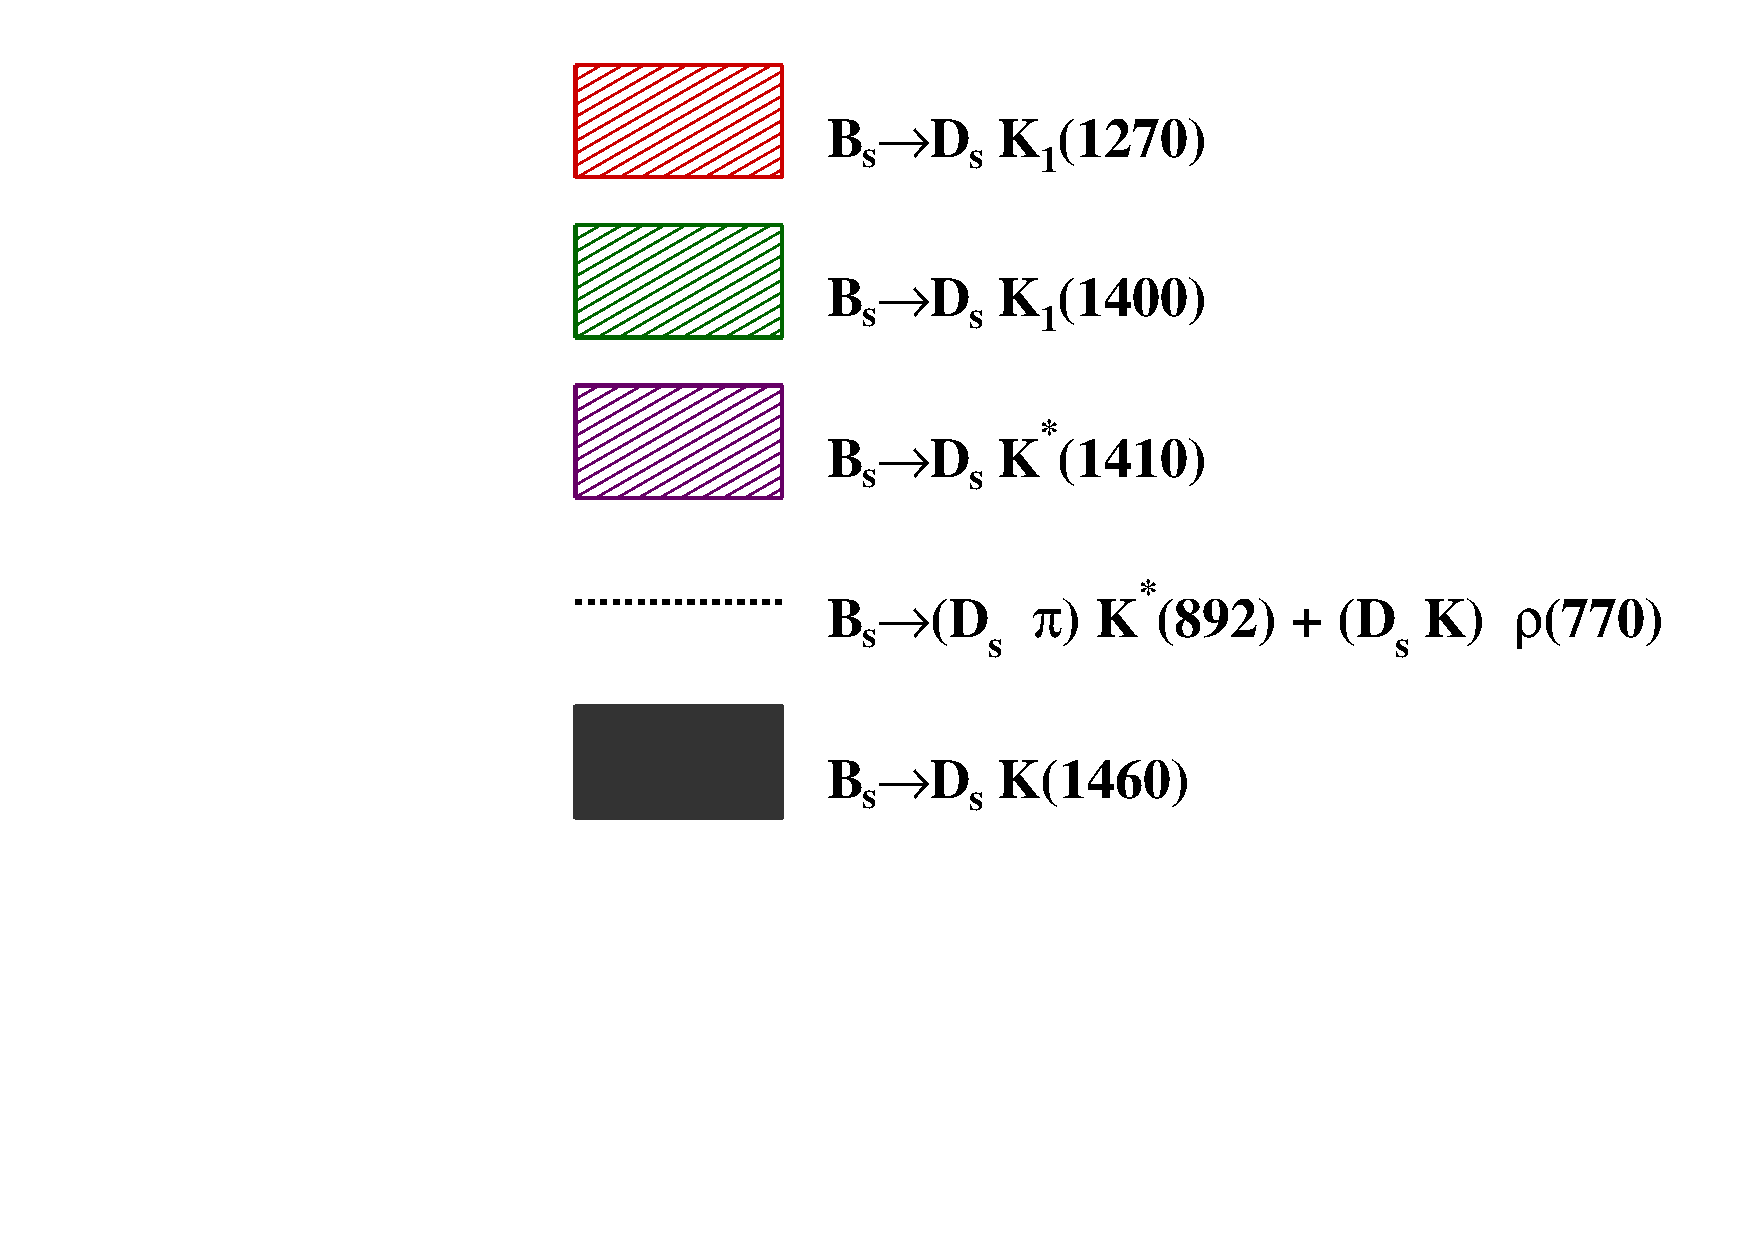
\includegraphics[width=0.32\textwidth, height = !]{figs/lassoFit/LASSO/leg.pdf} 
		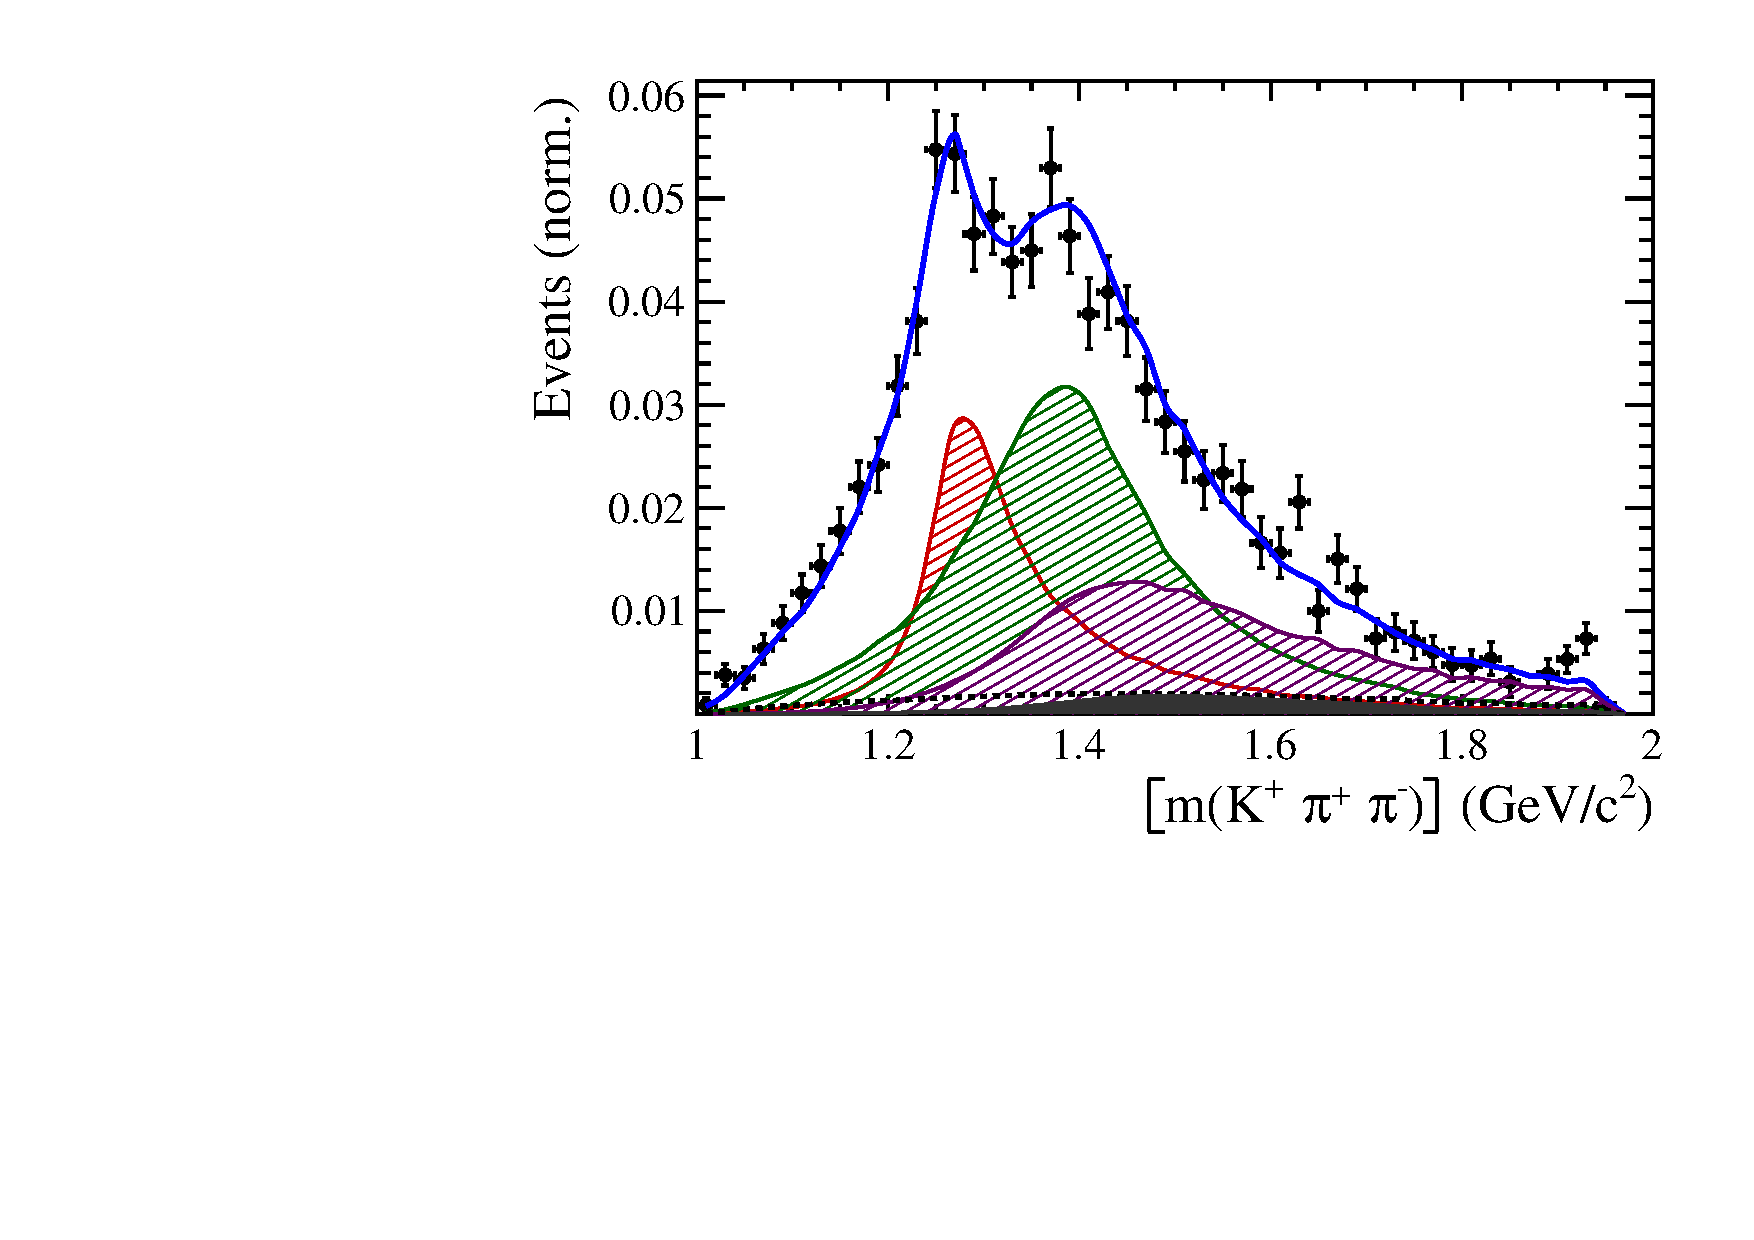
\includegraphics[width=0.32\textwidth, height = !]{figs/lassoFit/LASSO/m_Kpipi_mod.pdf} 
		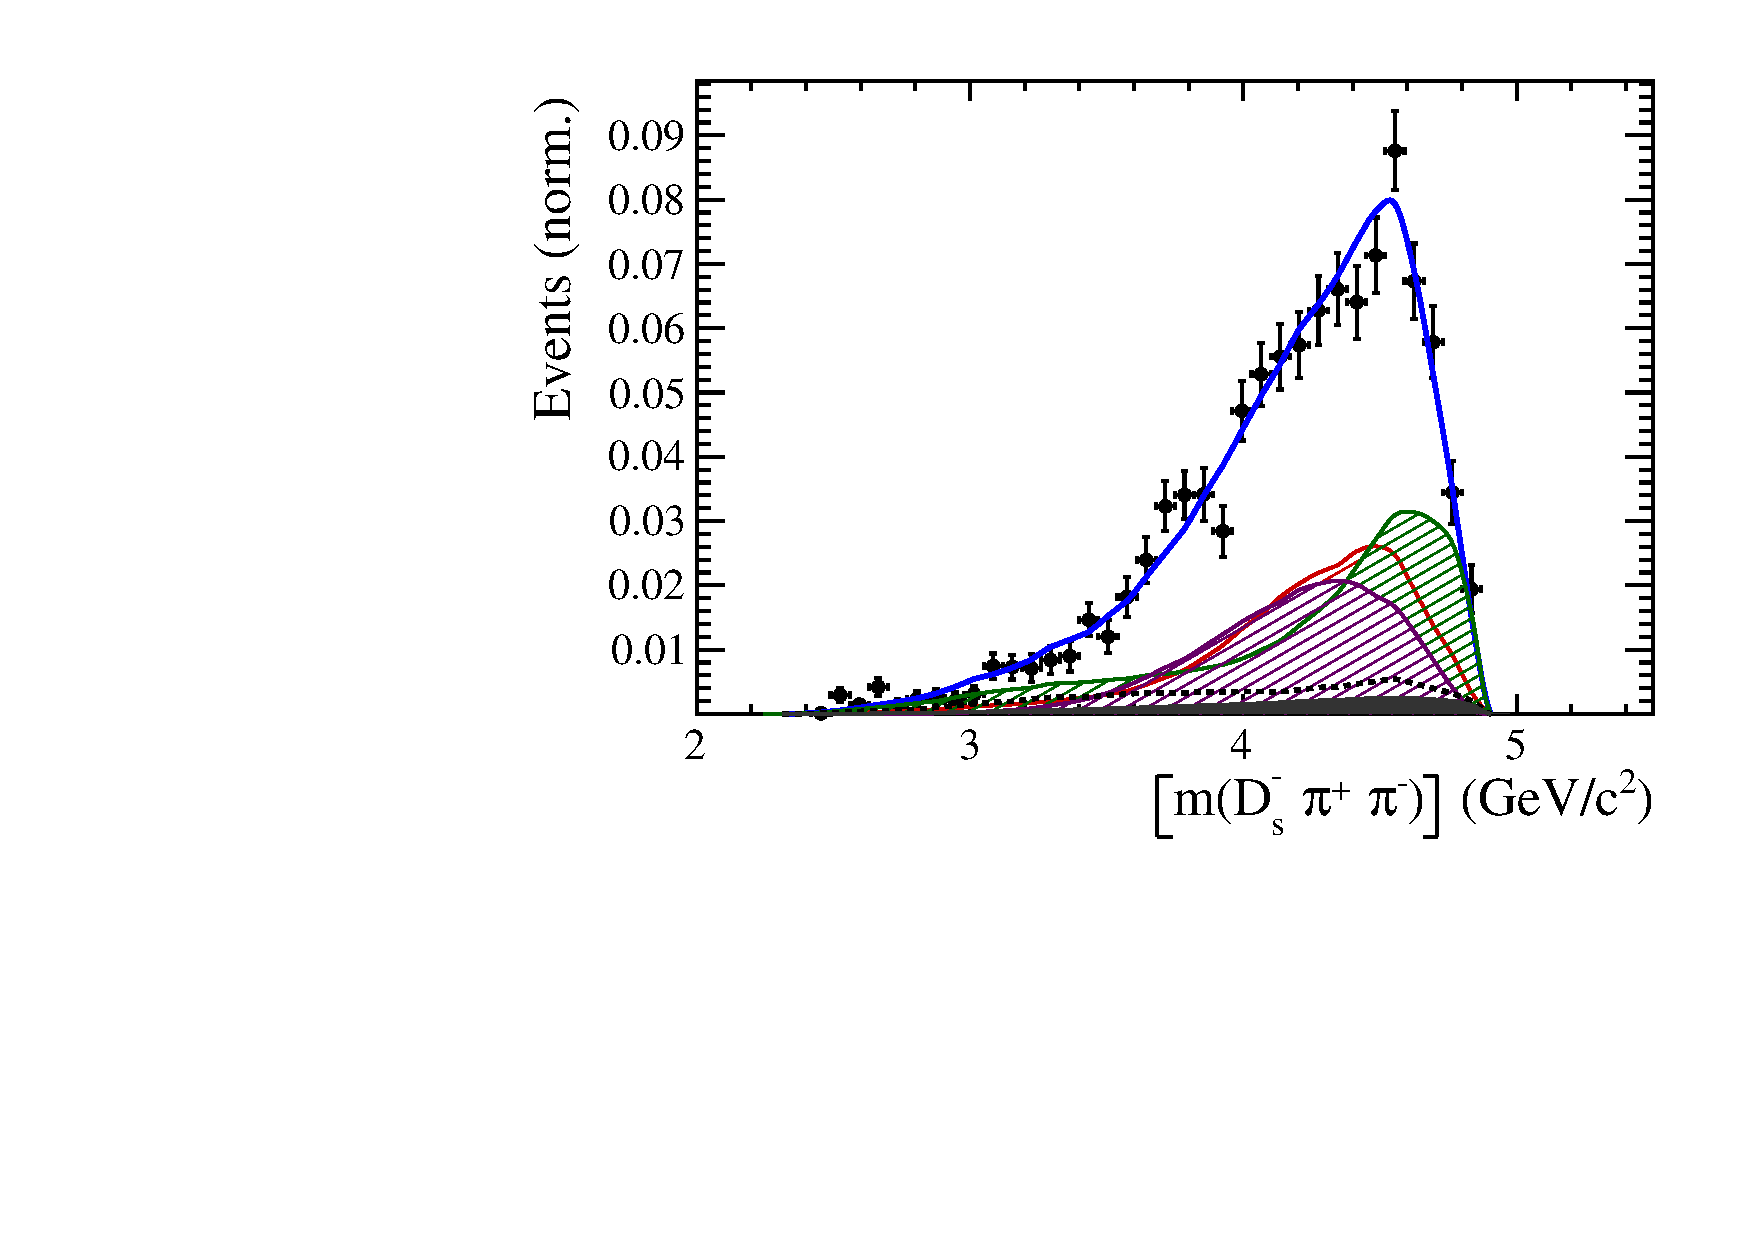
\includegraphics[width=0.32\textwidth, height = !]{figs/lassoFit/LASSO/m_Dspipi_mod.pdf} 
%		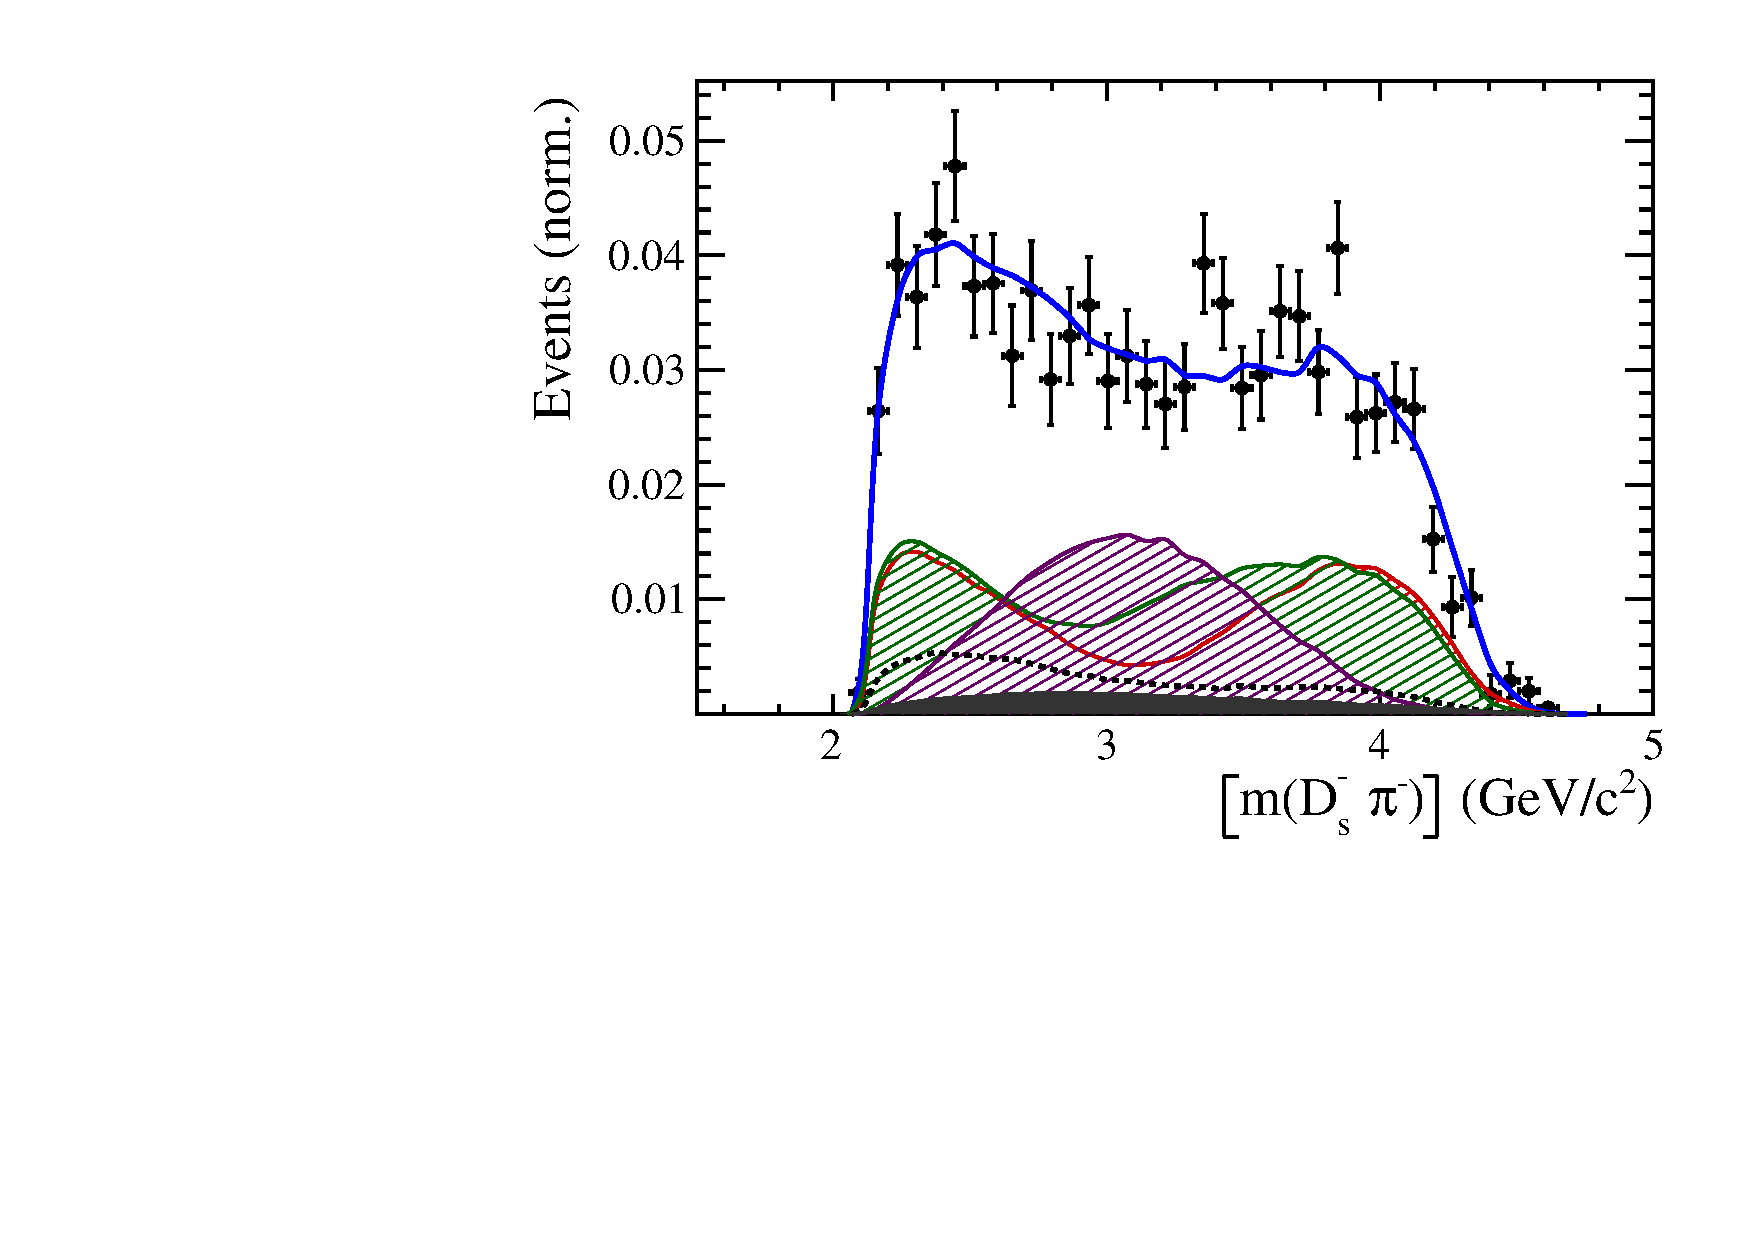
\includegraphics[width=0.32\textwidth, height = !]{figs/lassoFit/LASSO/m_Dspim_mod.pdf} 

		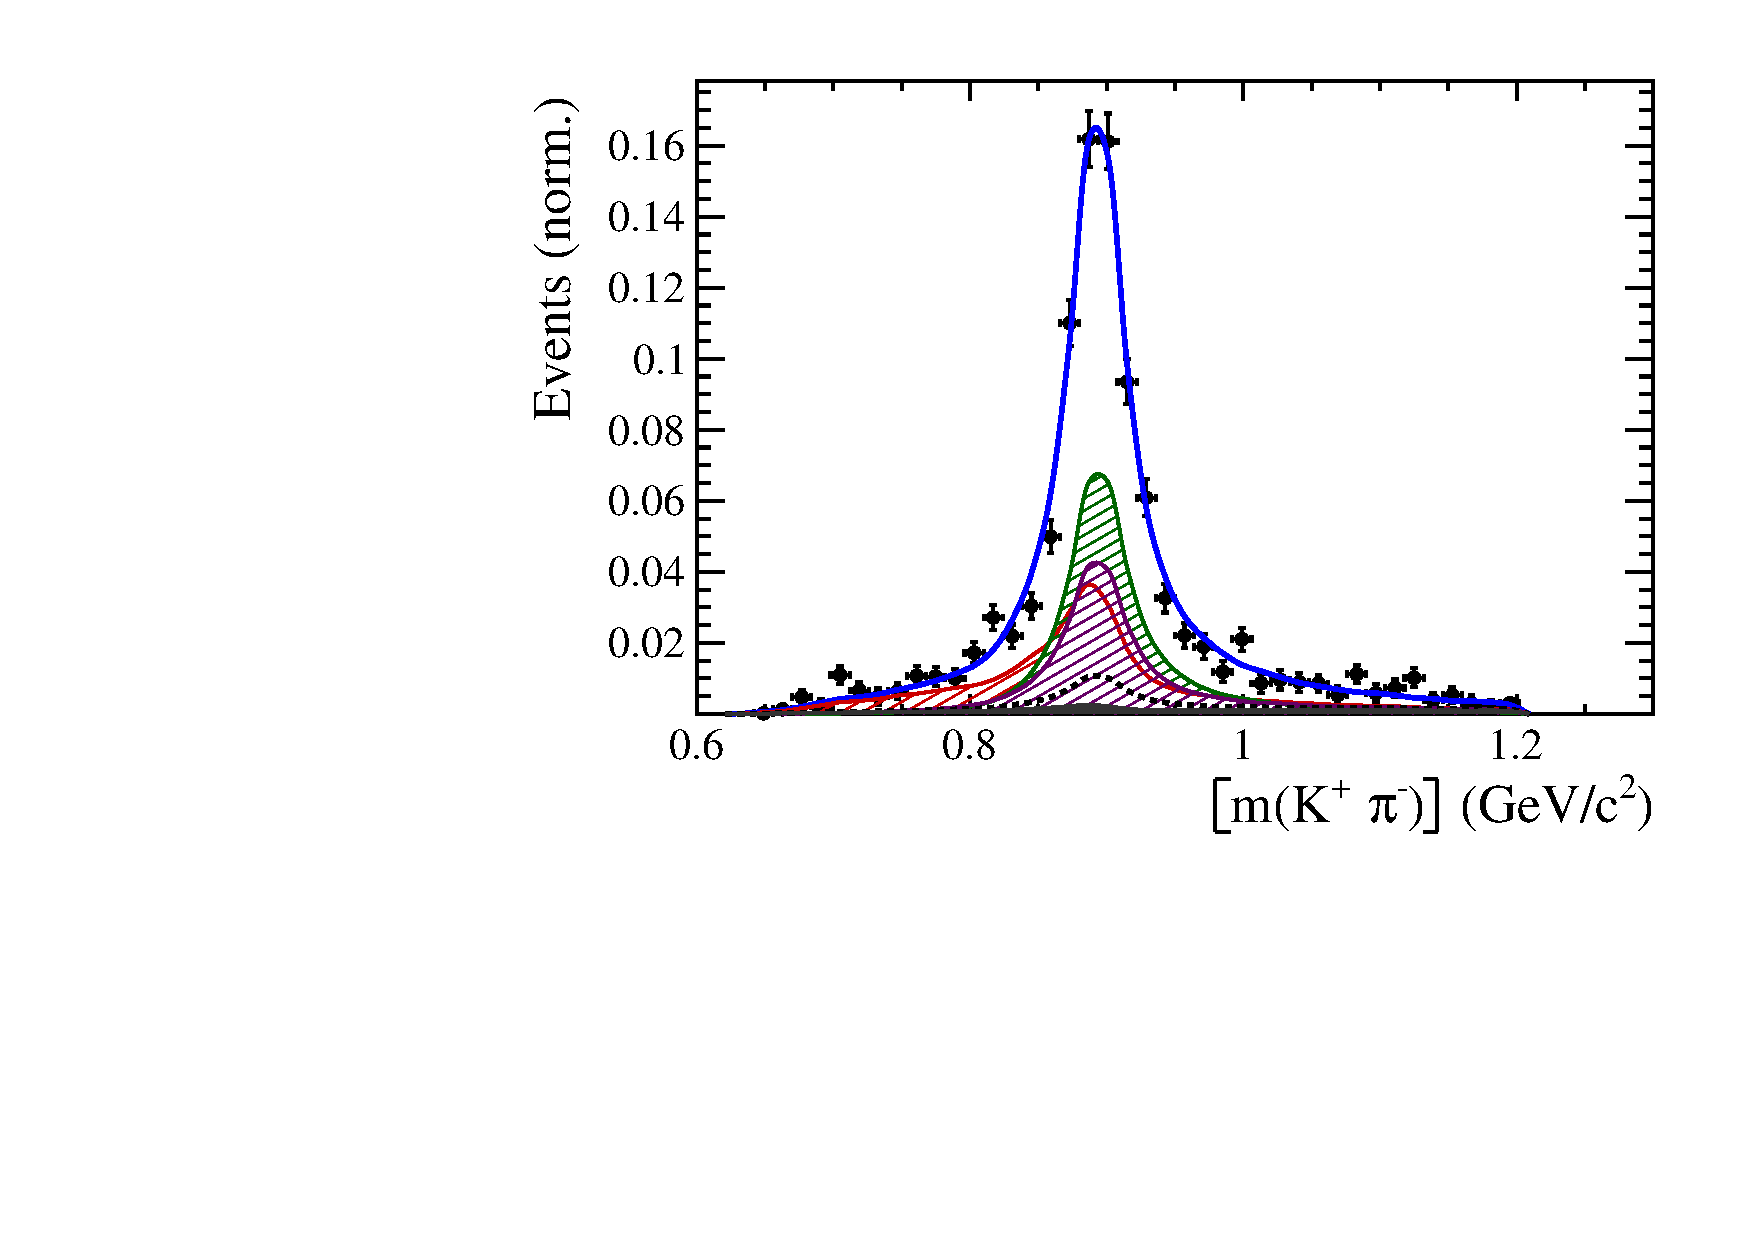
\includegraphics[width=0.32\textwidth, height = !]{figs/lassoFit/LASSO/m_Kpi_mod.pdf} 
		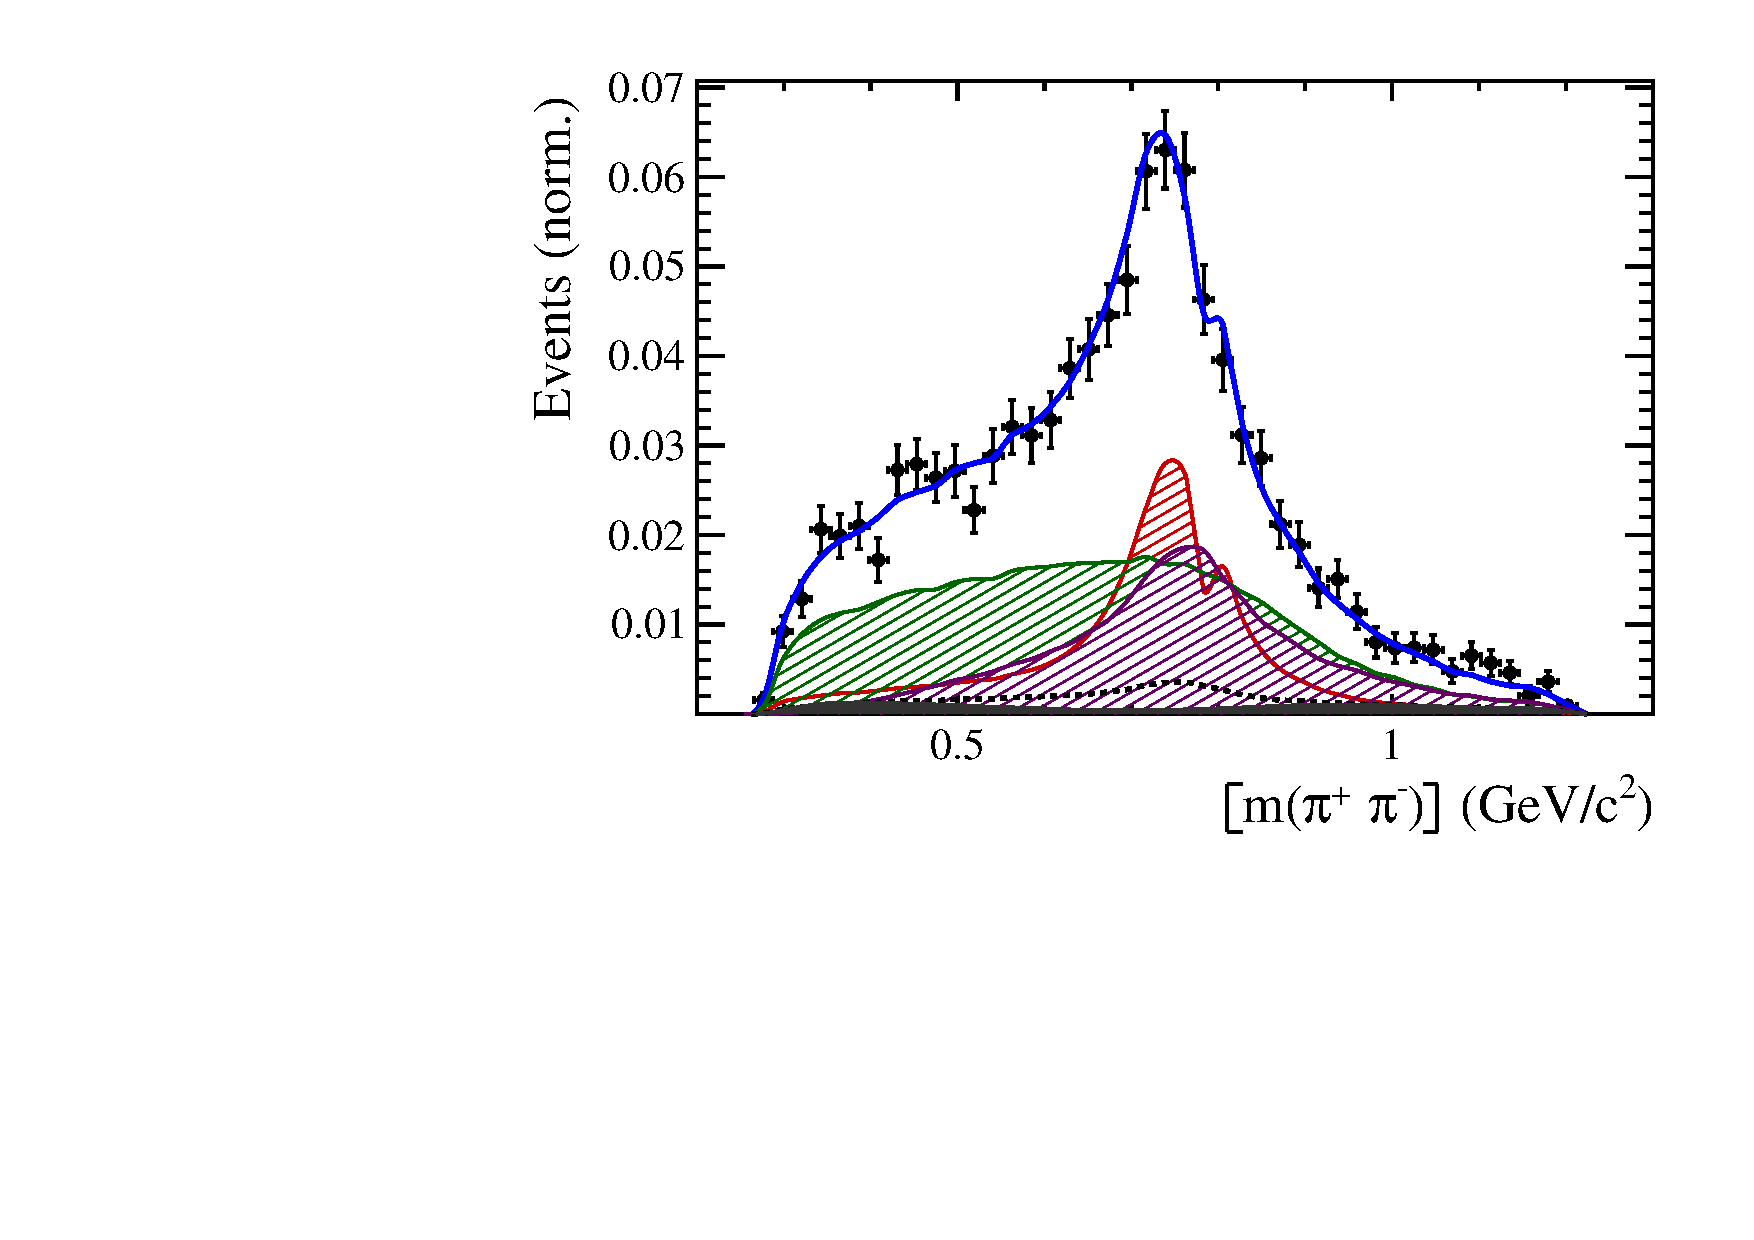
\includegraphics[width=0.32\textwidth, height = !]{figs/lassoFit/LASSO/m_pipi_mod.pdf} 
		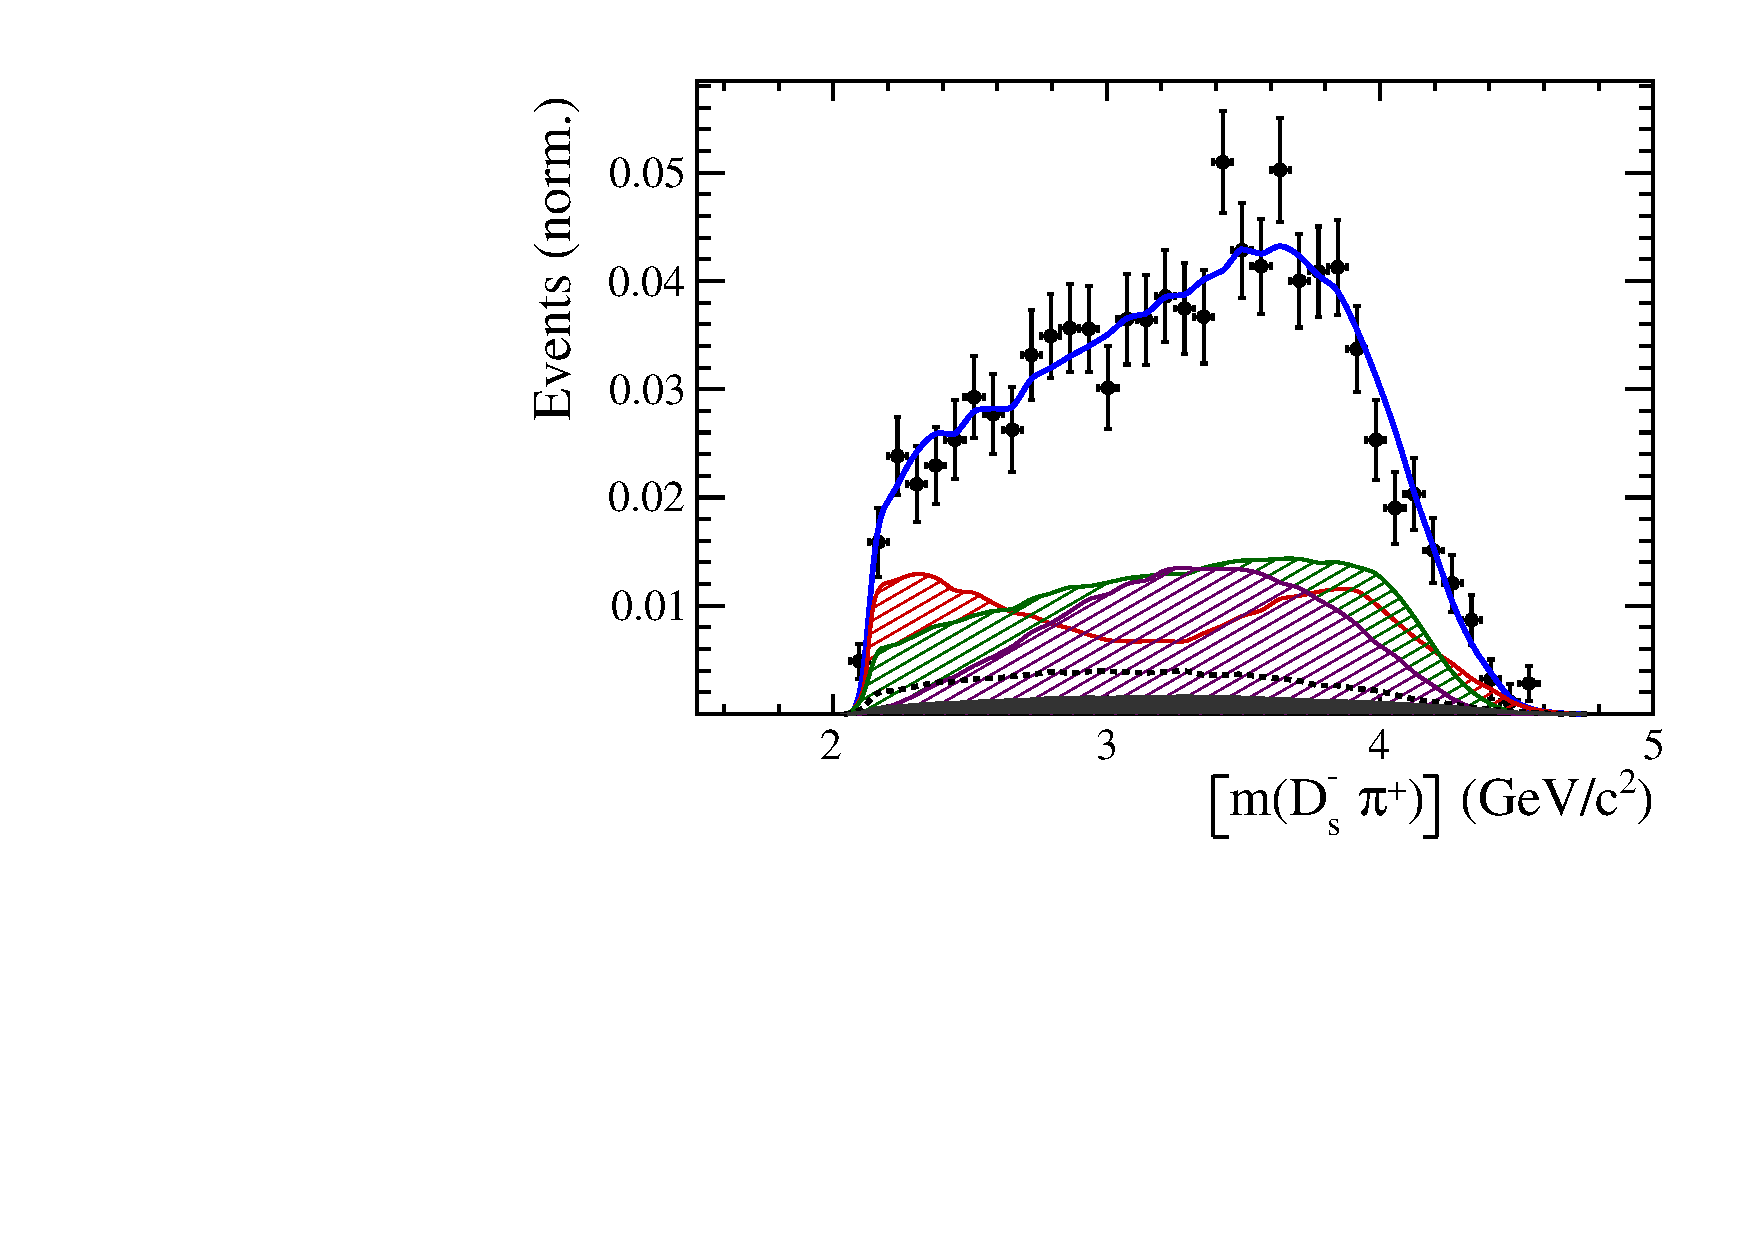
\includegraphics[width=0.32\textwidth, height = !]{figs/lassoFit/LASSO/m_Dspi_mod.pdf} 
		
		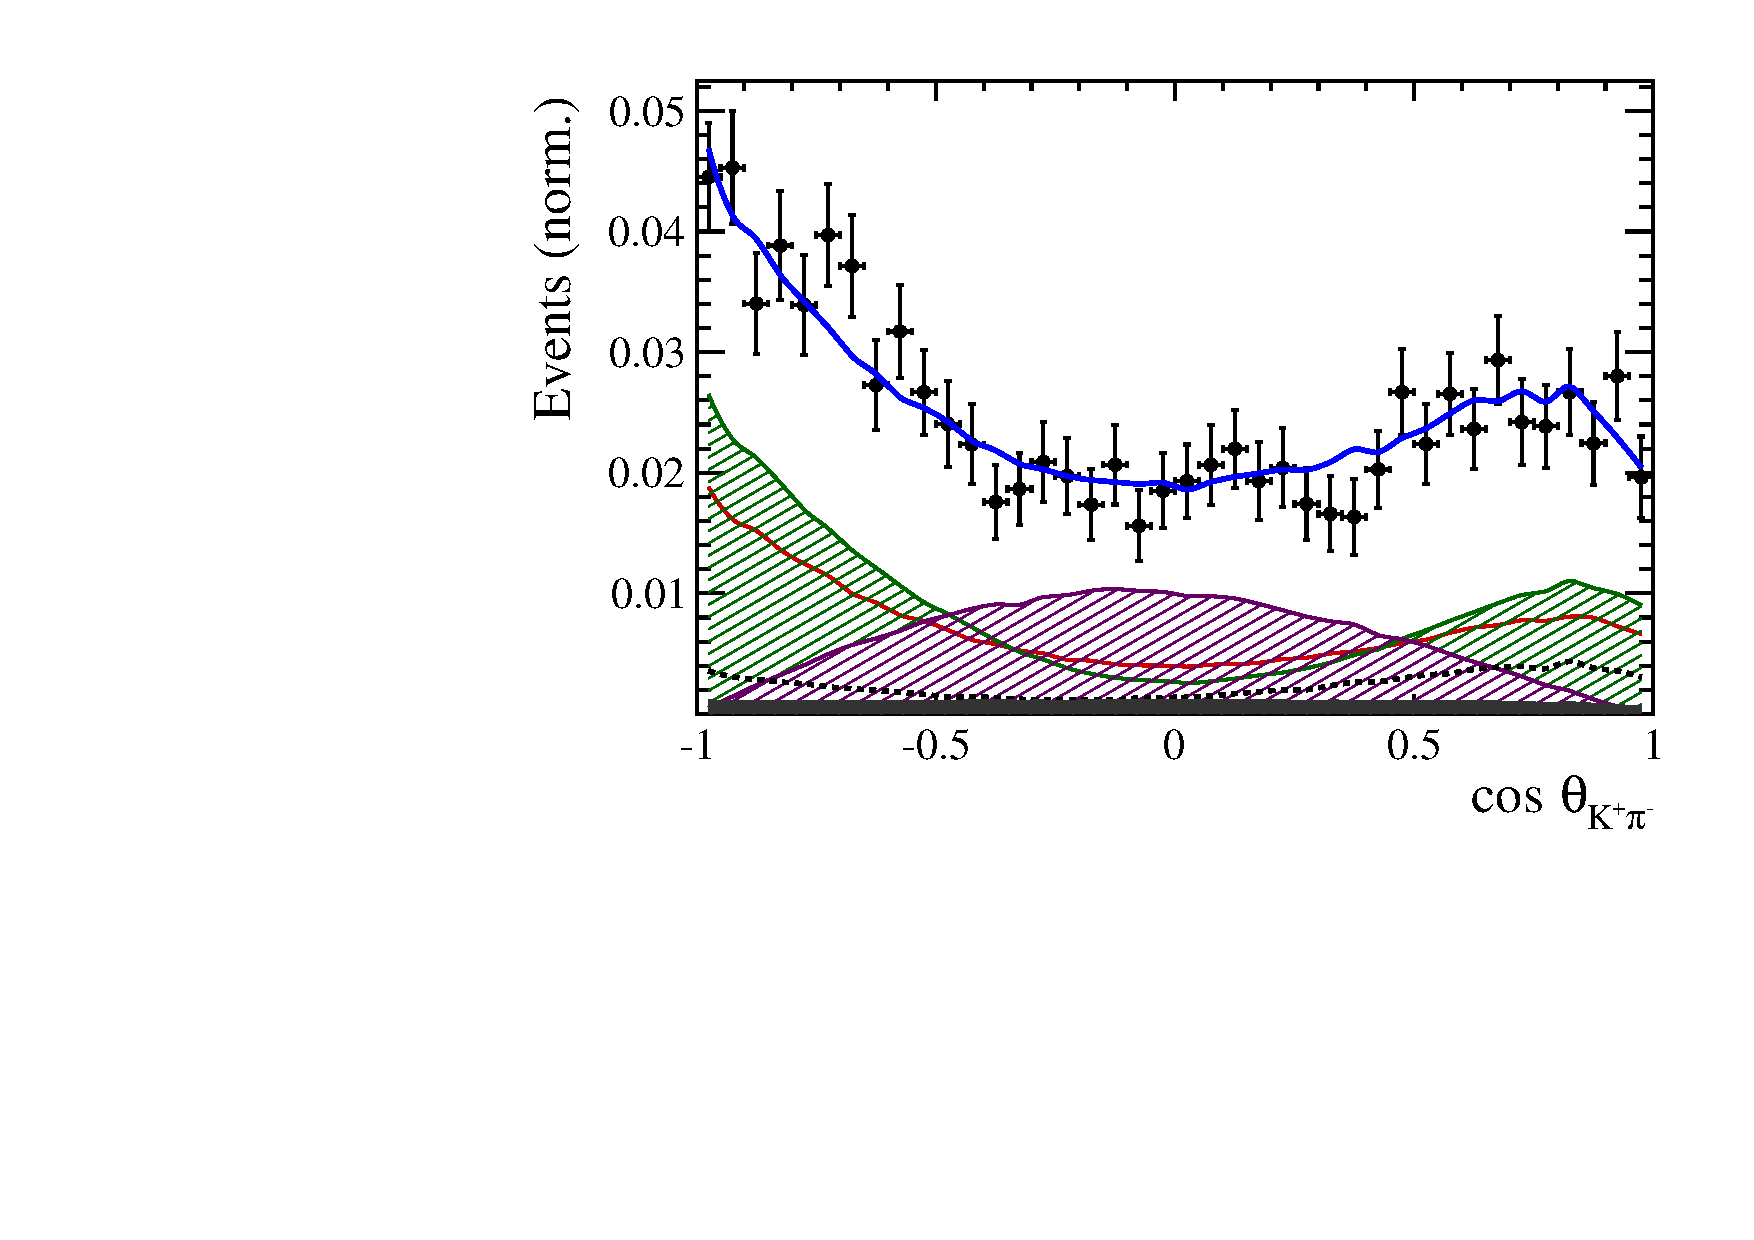
\includegraphics[width=0.32\textwidth, height = !]{figs/lassoFit/LASSO/h_cosTheta_Kpi_mod.pdf} 
		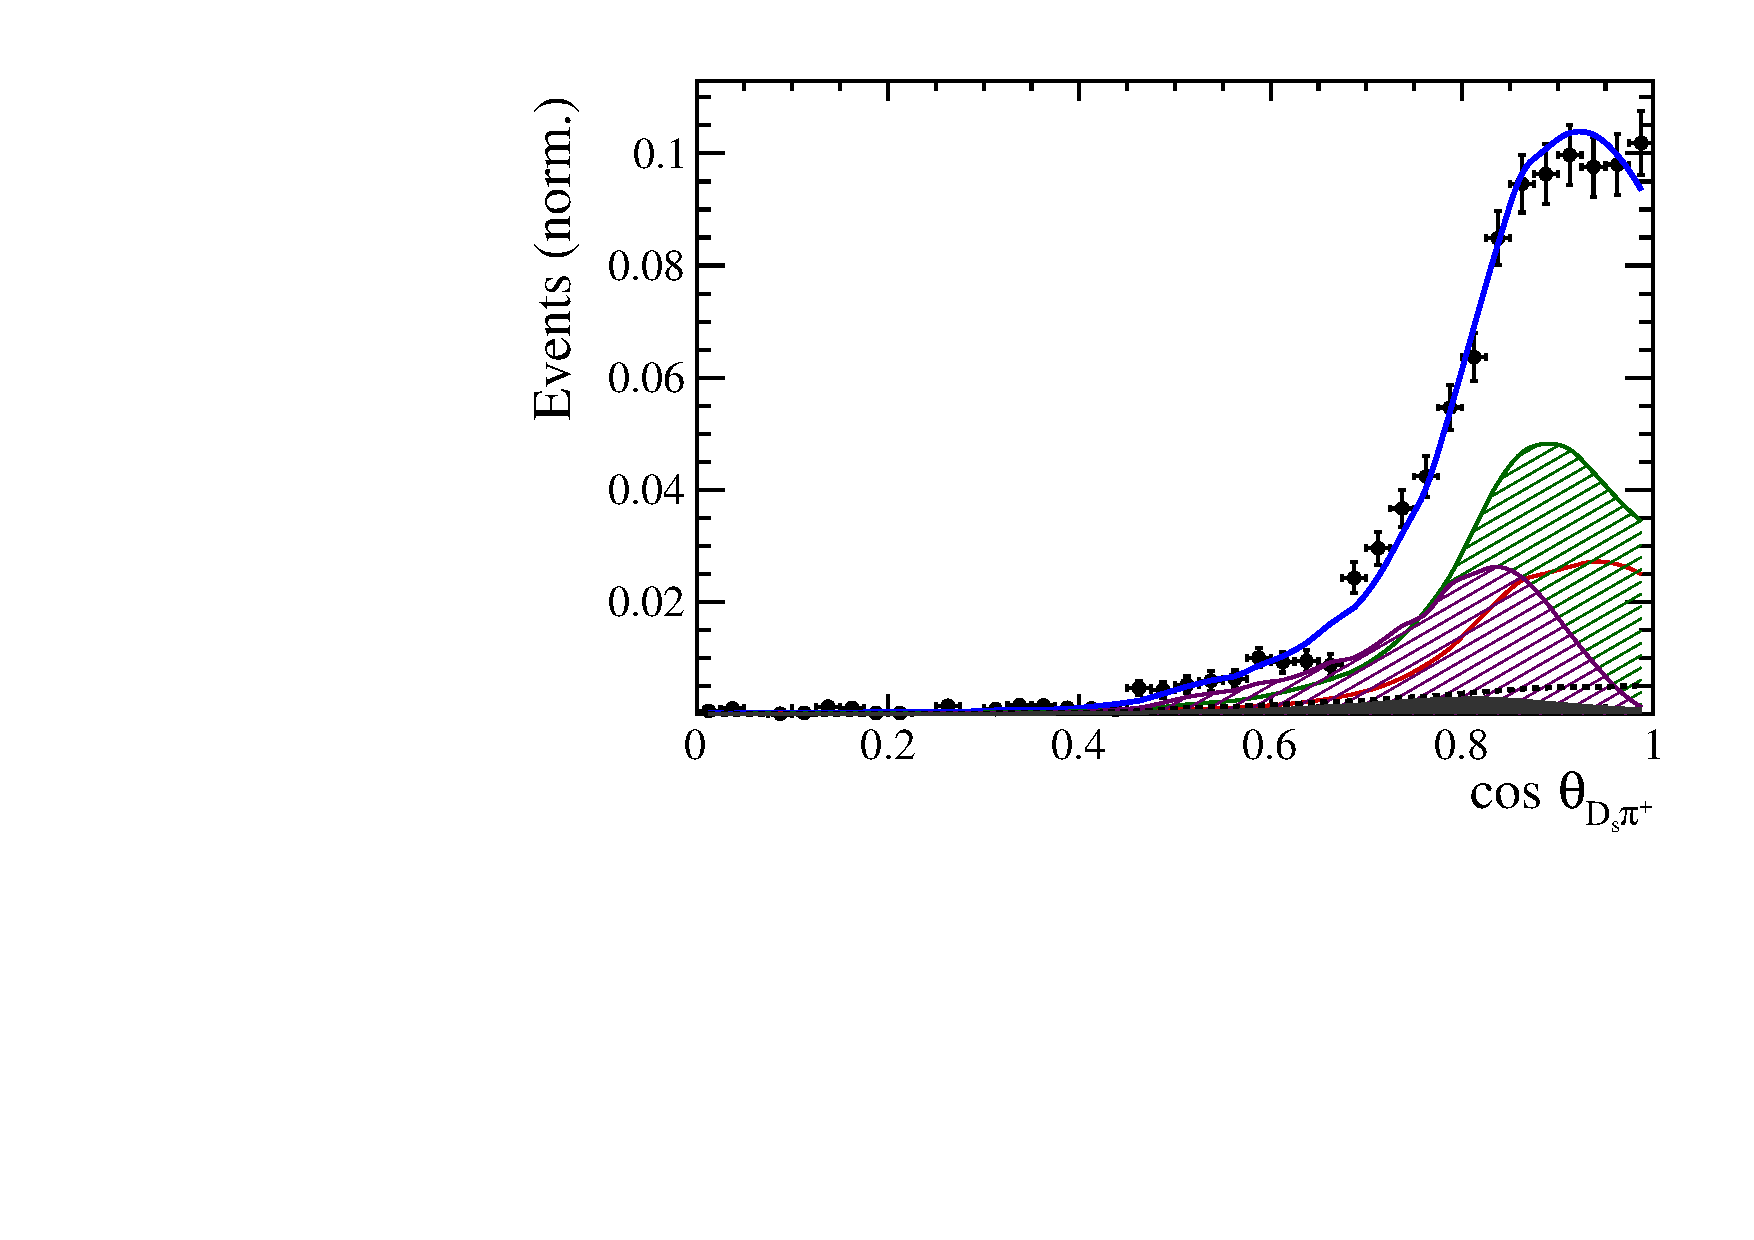
\includegraphics[width=0.32\textwidth, height = !]{figs/lassoFit/LASSO/h_cosTheta_Dspi_mod.pdf} 
		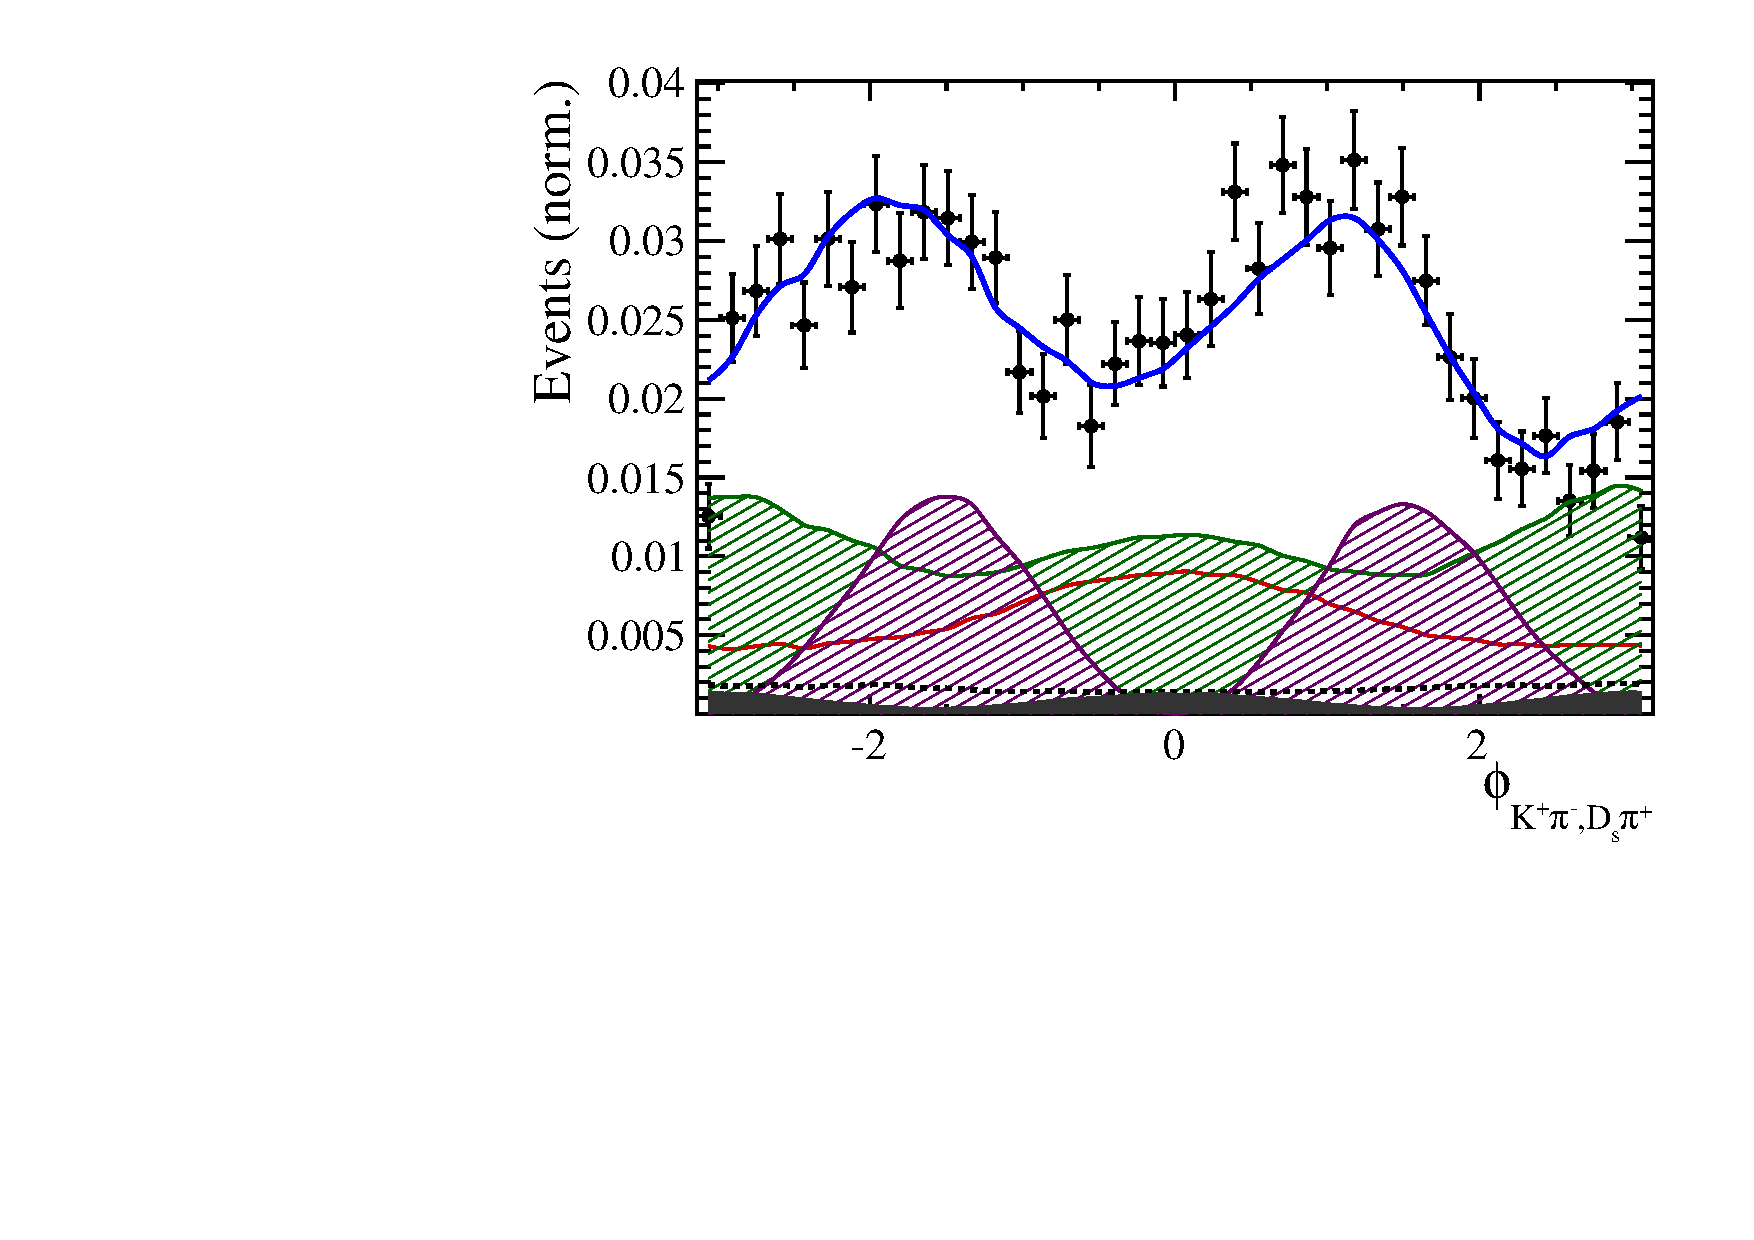
\includegraphics[width=0.32\textwidth, height = !]{figs/lassoFit/LASSO/h_phi_Kpi_Dspi_mod.pdf} 

		\caption{\small Projections of the fit result to the time-integrated and flavour averaged phase-space distribution of $B_s \to D_s K \pi \pi$  decays. } 		
				\label{fig:lassoFit}

	\centering
		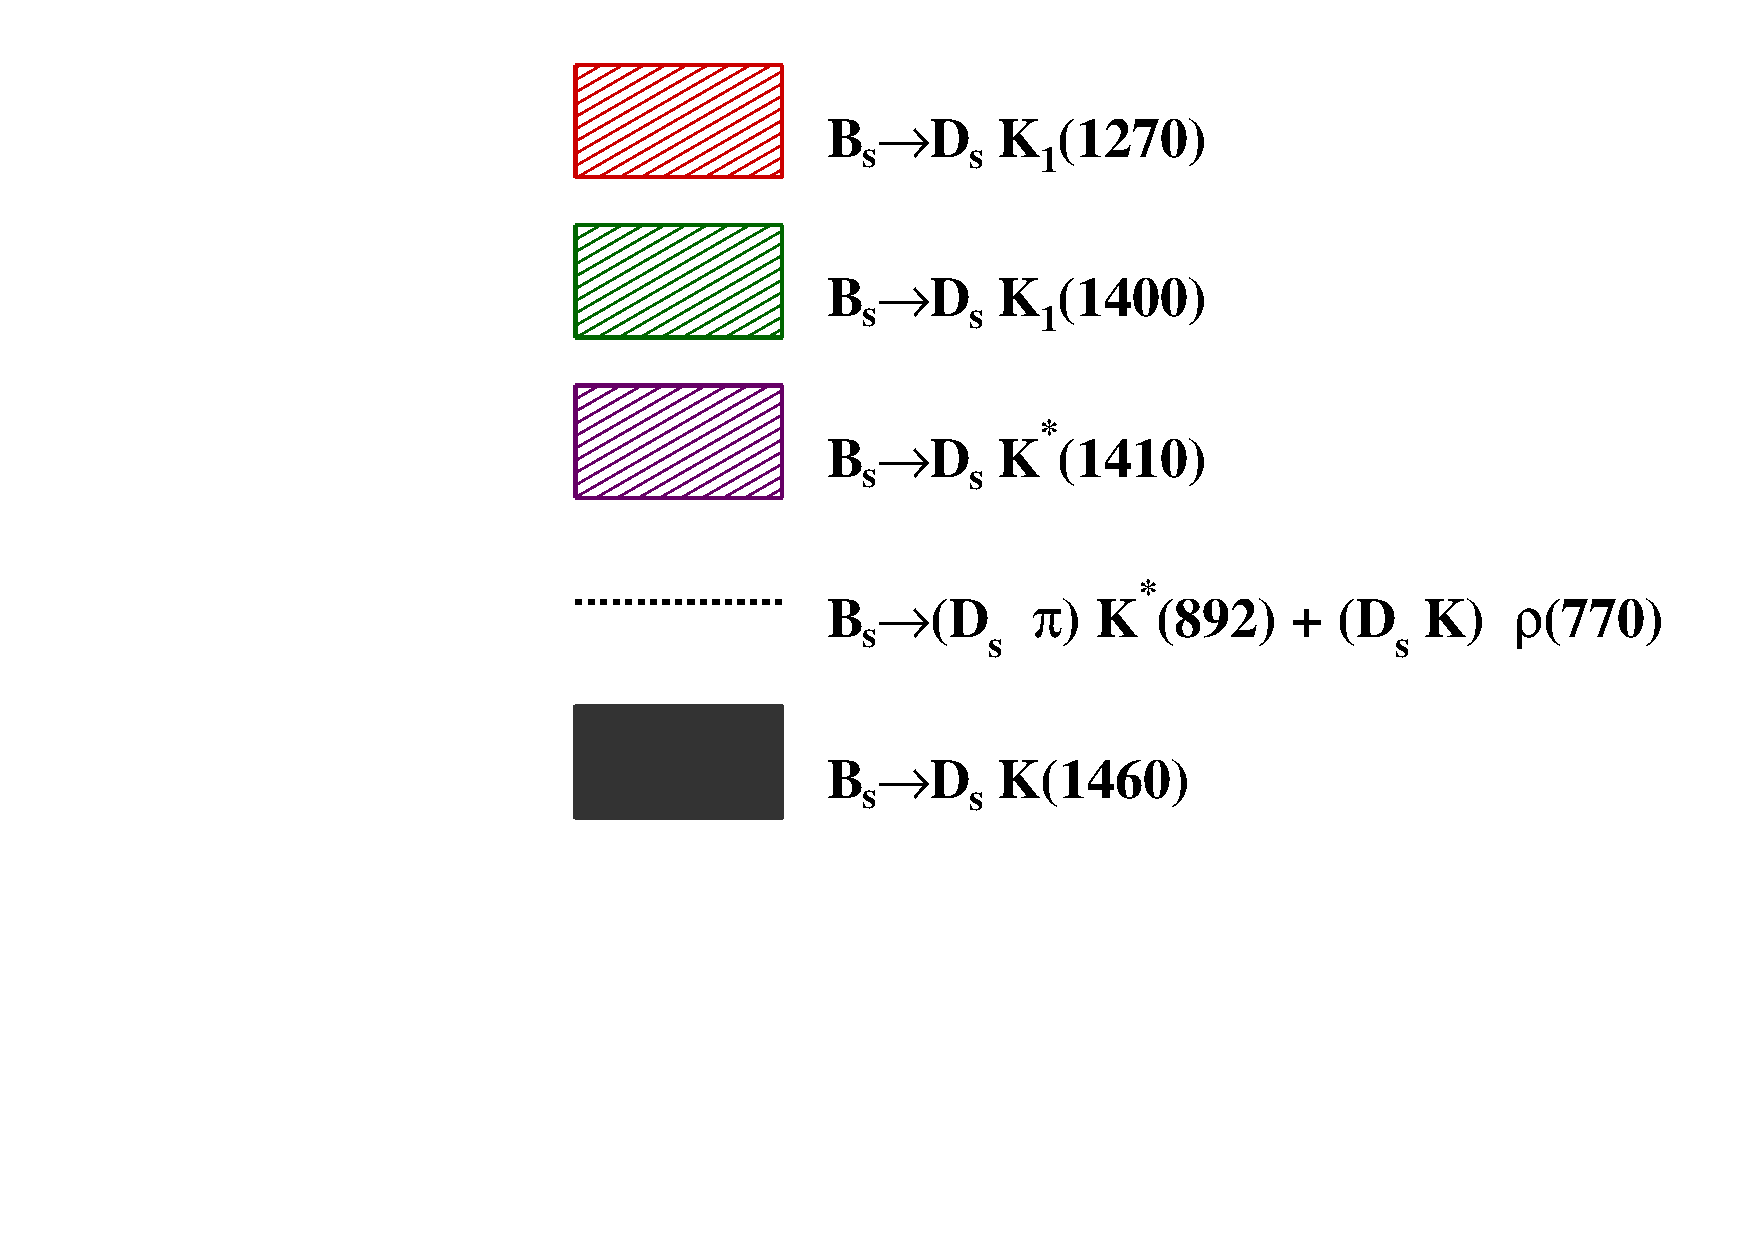
\includegraphics[width=0.32\textwidth, height = !]{figs/lassoFit/LASSO/leg.pdf} 
		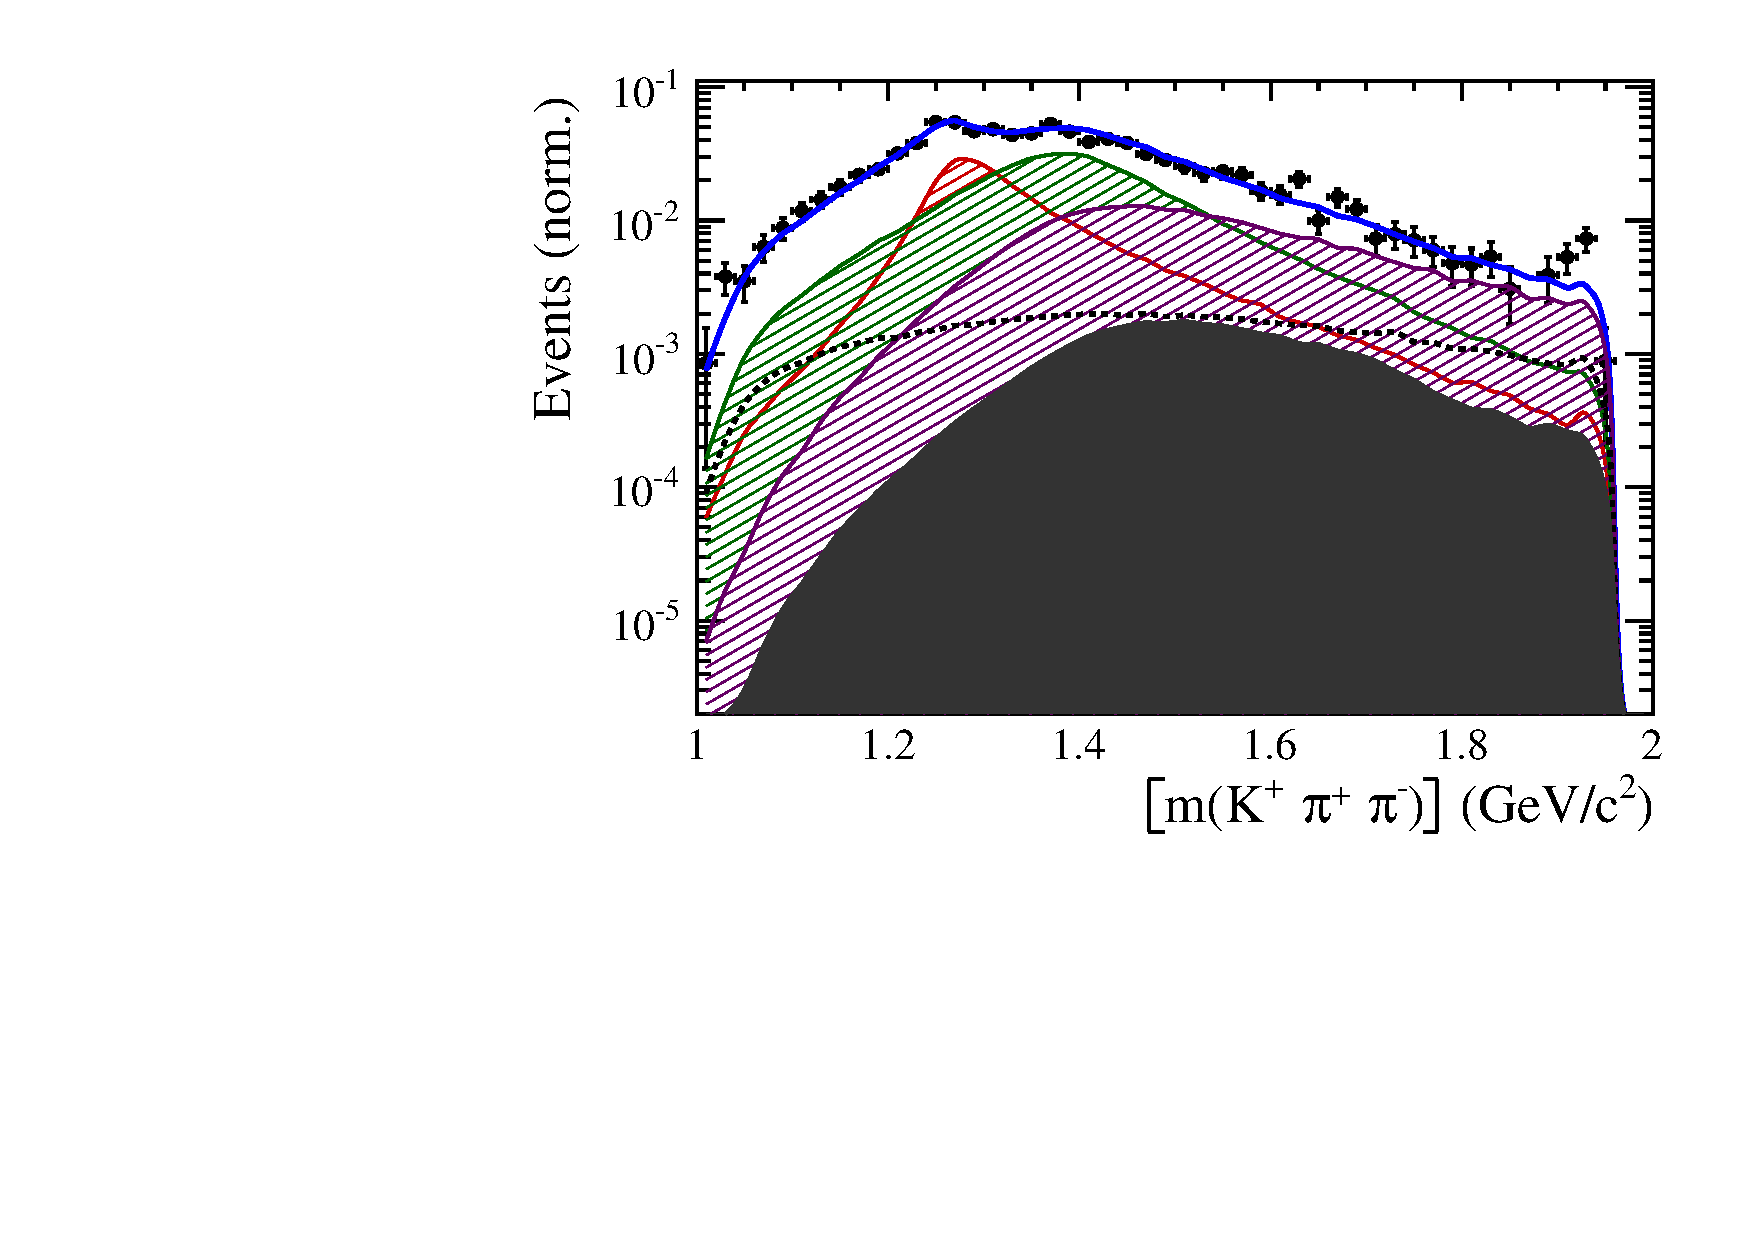
\includegraphics[width=0.32\textwidth, height = !]{figs/lassoFit/LASSO/m_Kpipi_mod_log.pdf} 
		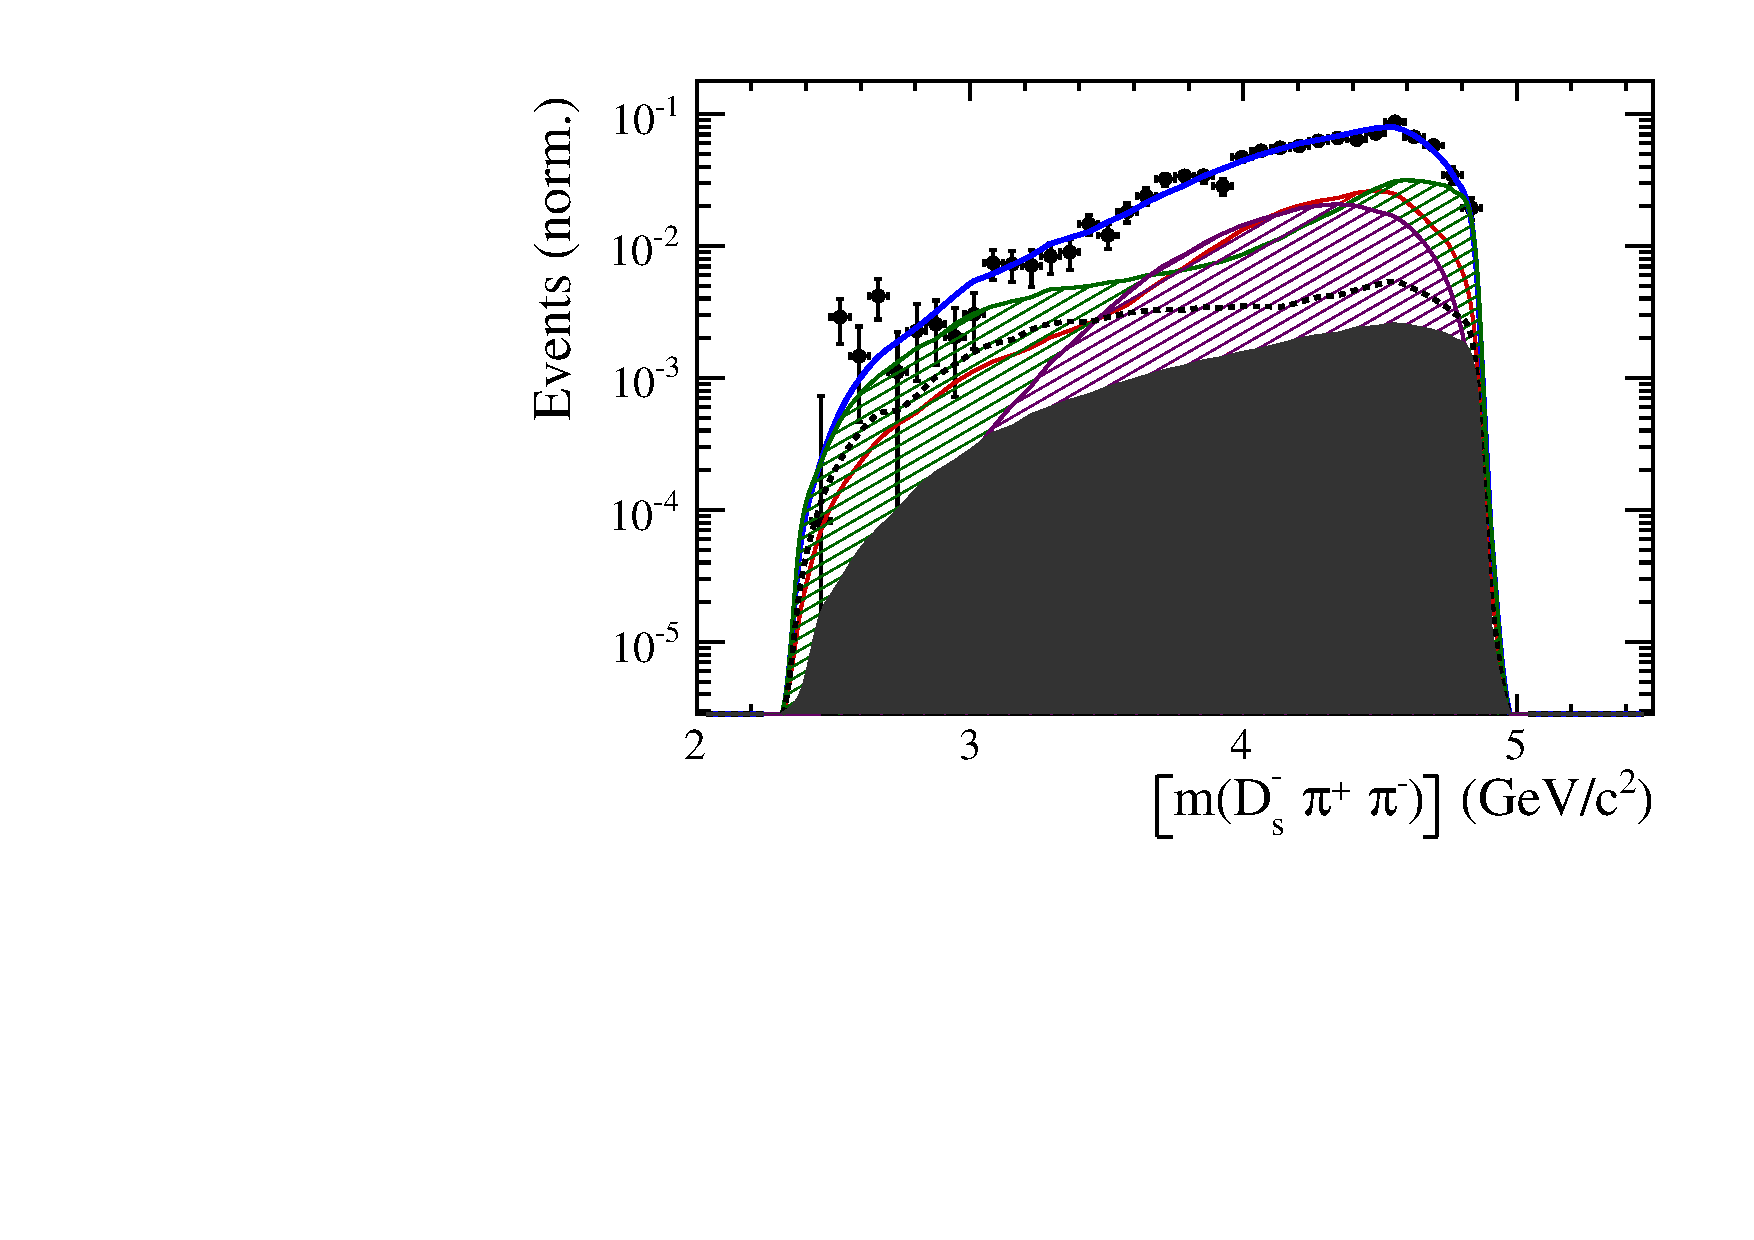
\includegraphics[width=0.32\textwidth, height = !]{figs/lassoFit/LASSO/m_Dspipi_mod_log.pdf} 
%		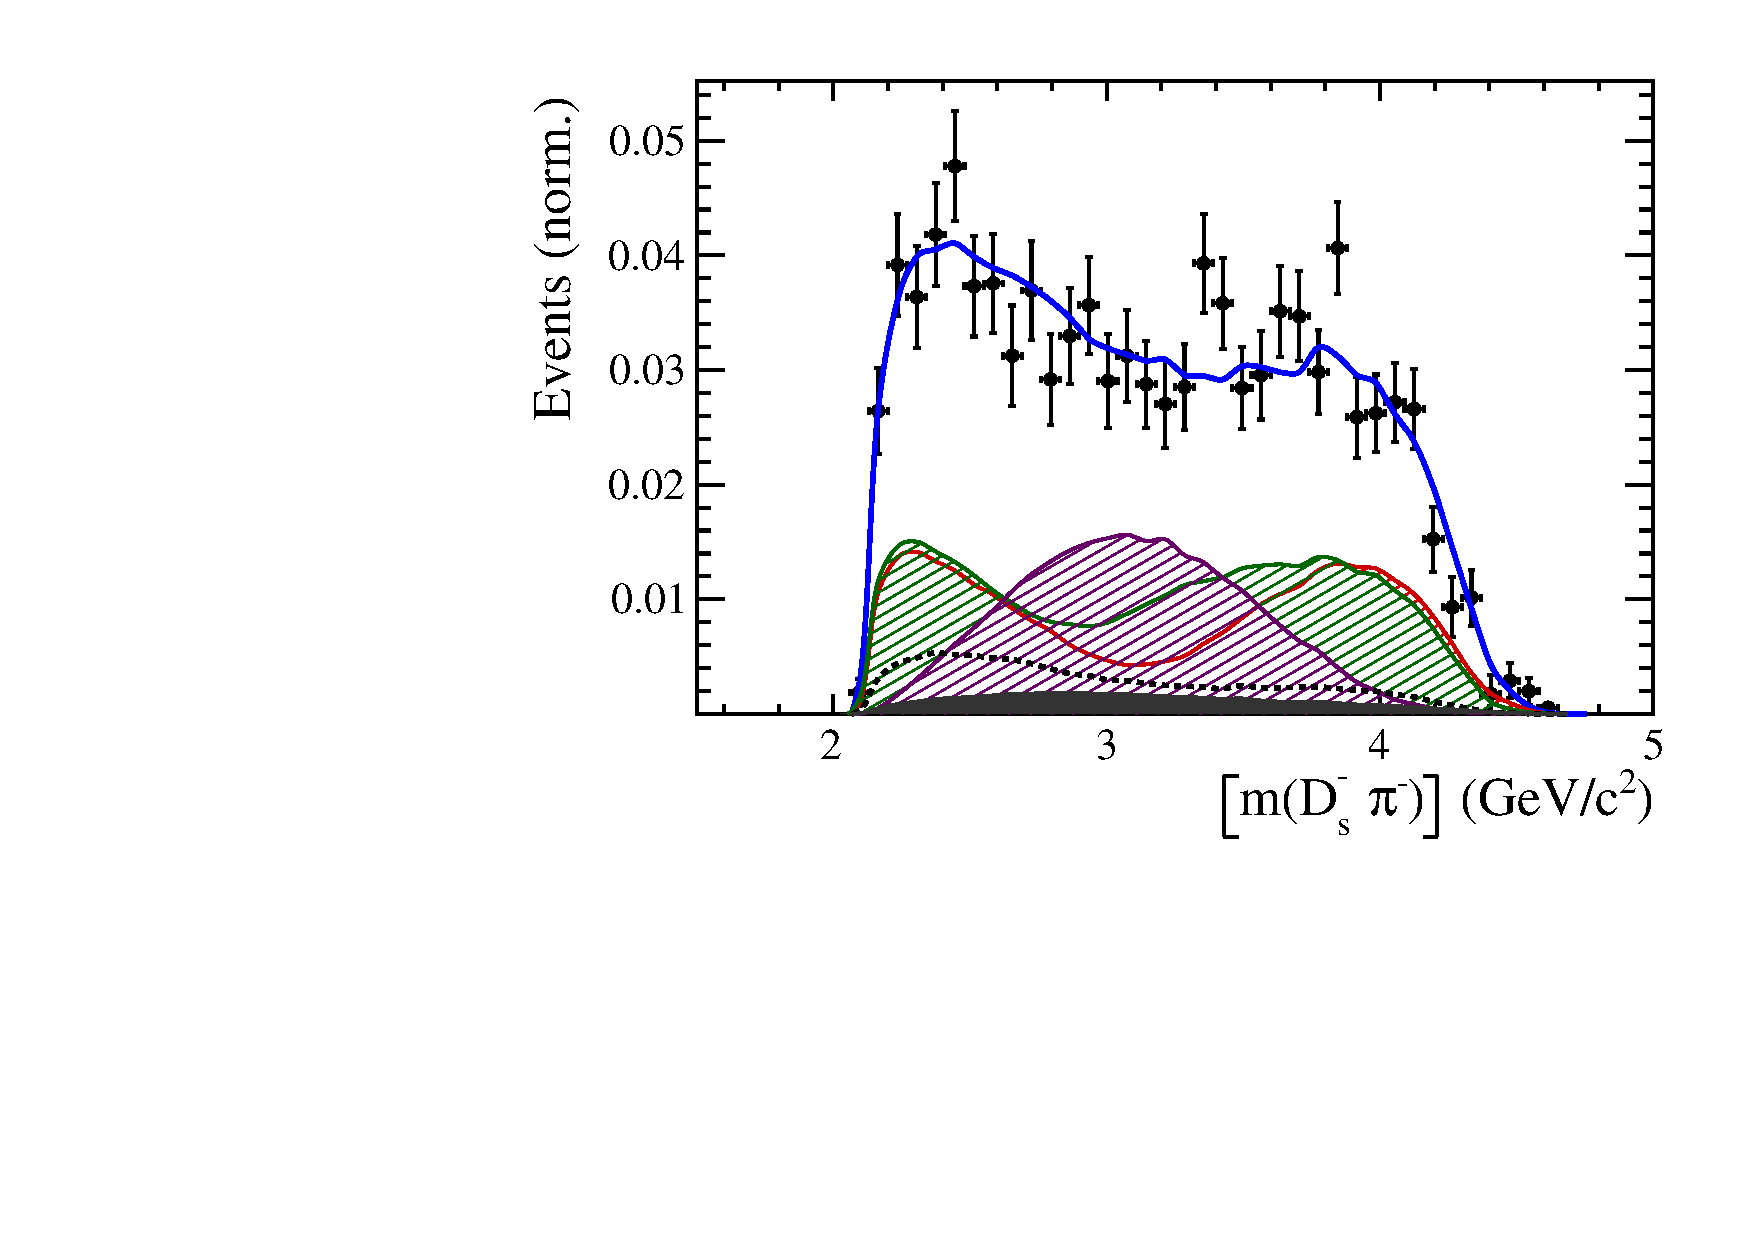
\includegraphics[width=0.32\textwidth, height = !]{figs/lassoFit/LASSO/m_Dspim_mod.pdf} 

		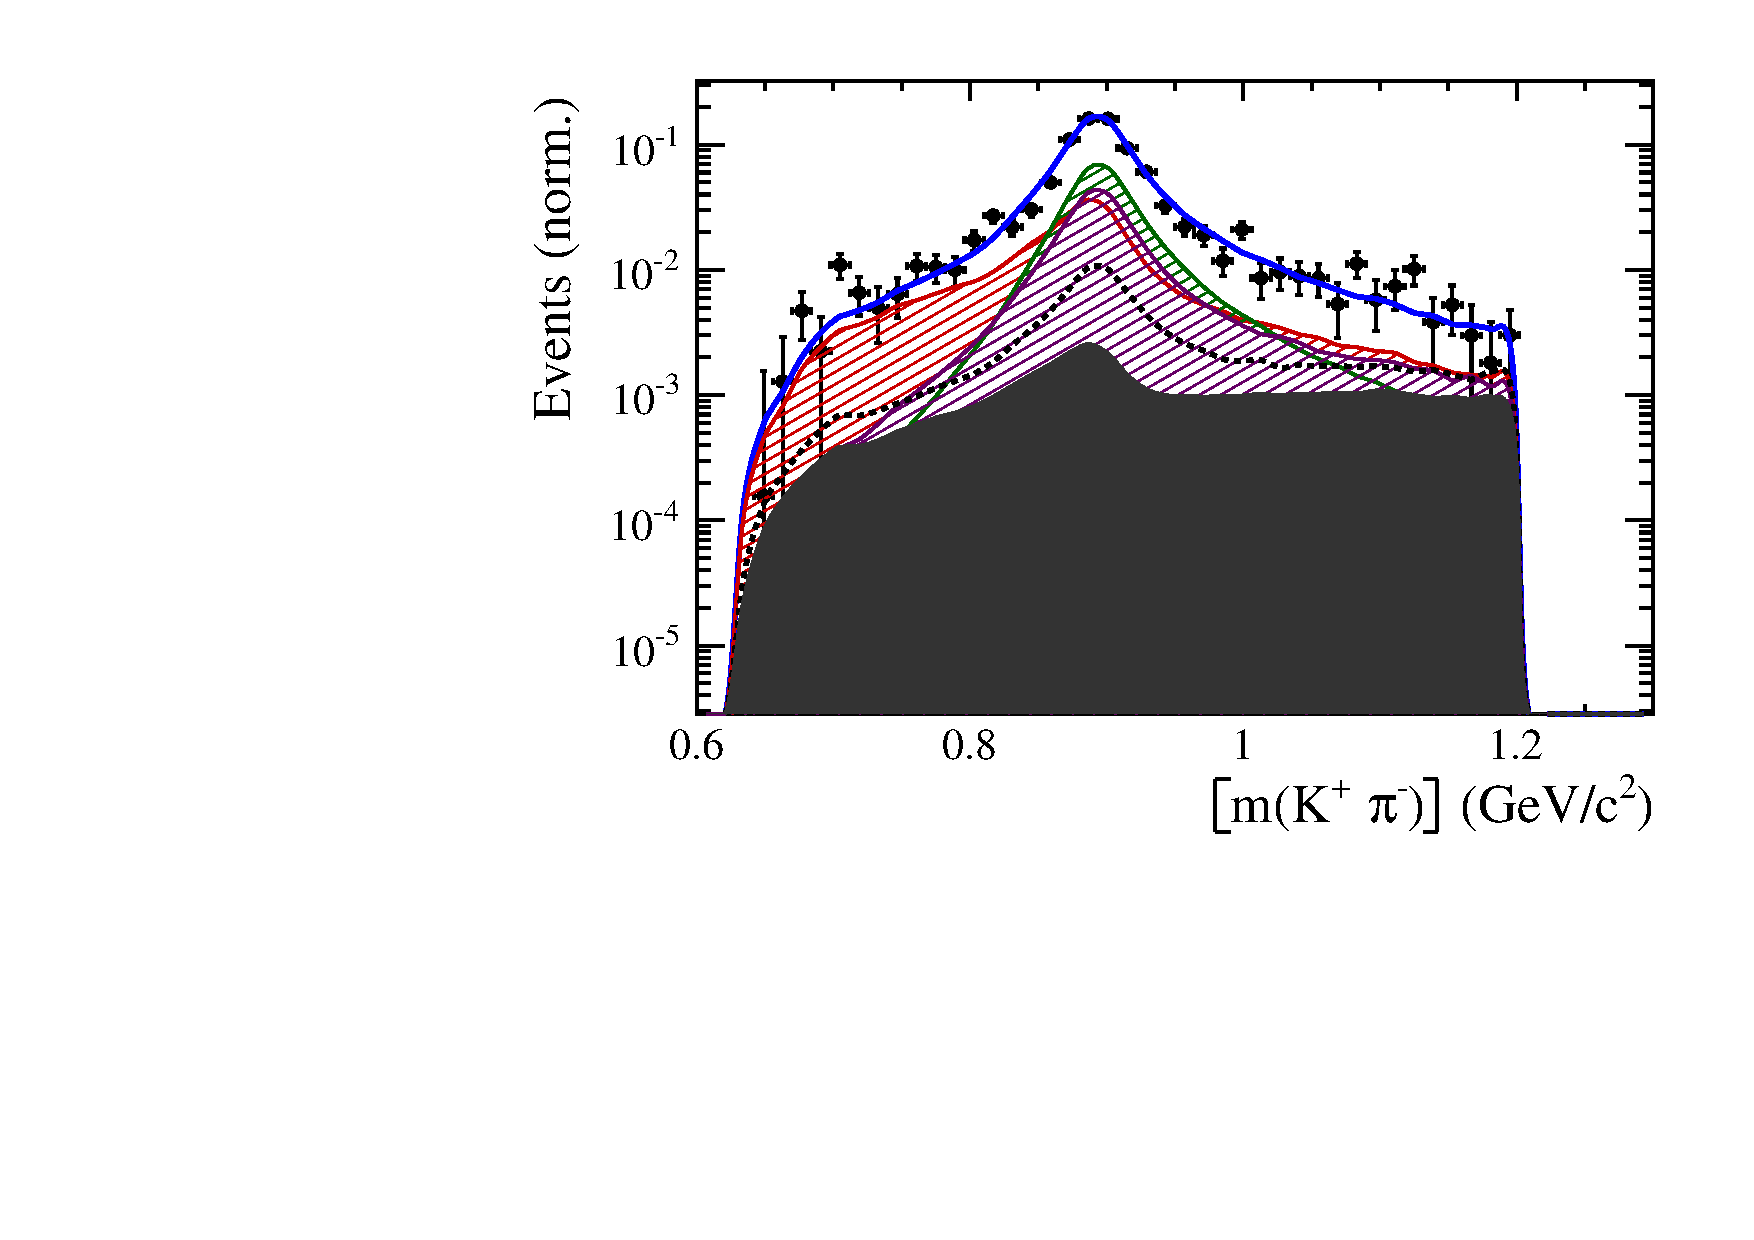
\includegraphics[width=0.32\textwidth, height = !]{figs/lassoFit/LASSO/m_Kpi_mod_log.pdf} 
		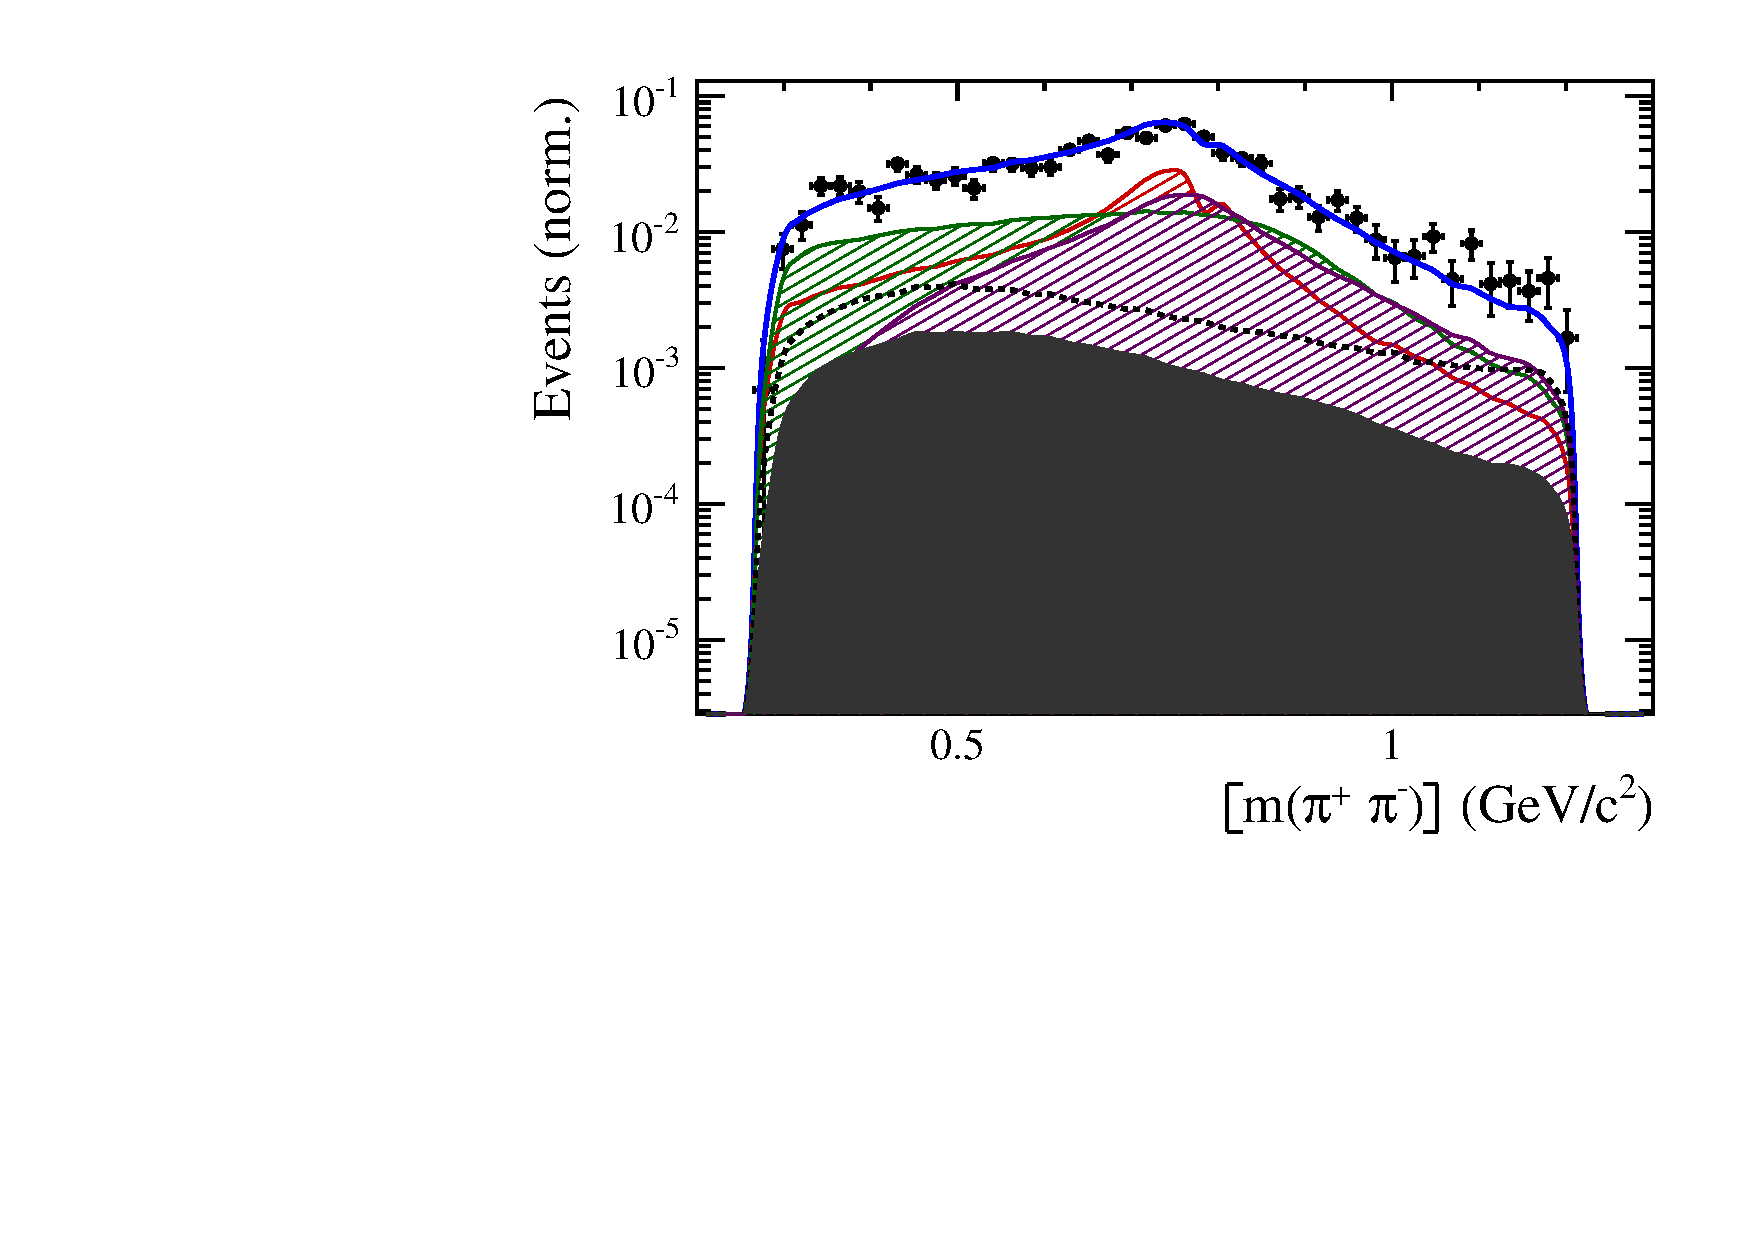
\includegraphics[width=0.32\textwidth, height = !]{figs/lassoFit/LASSO/m_pipi_mod_log.pdf} 
		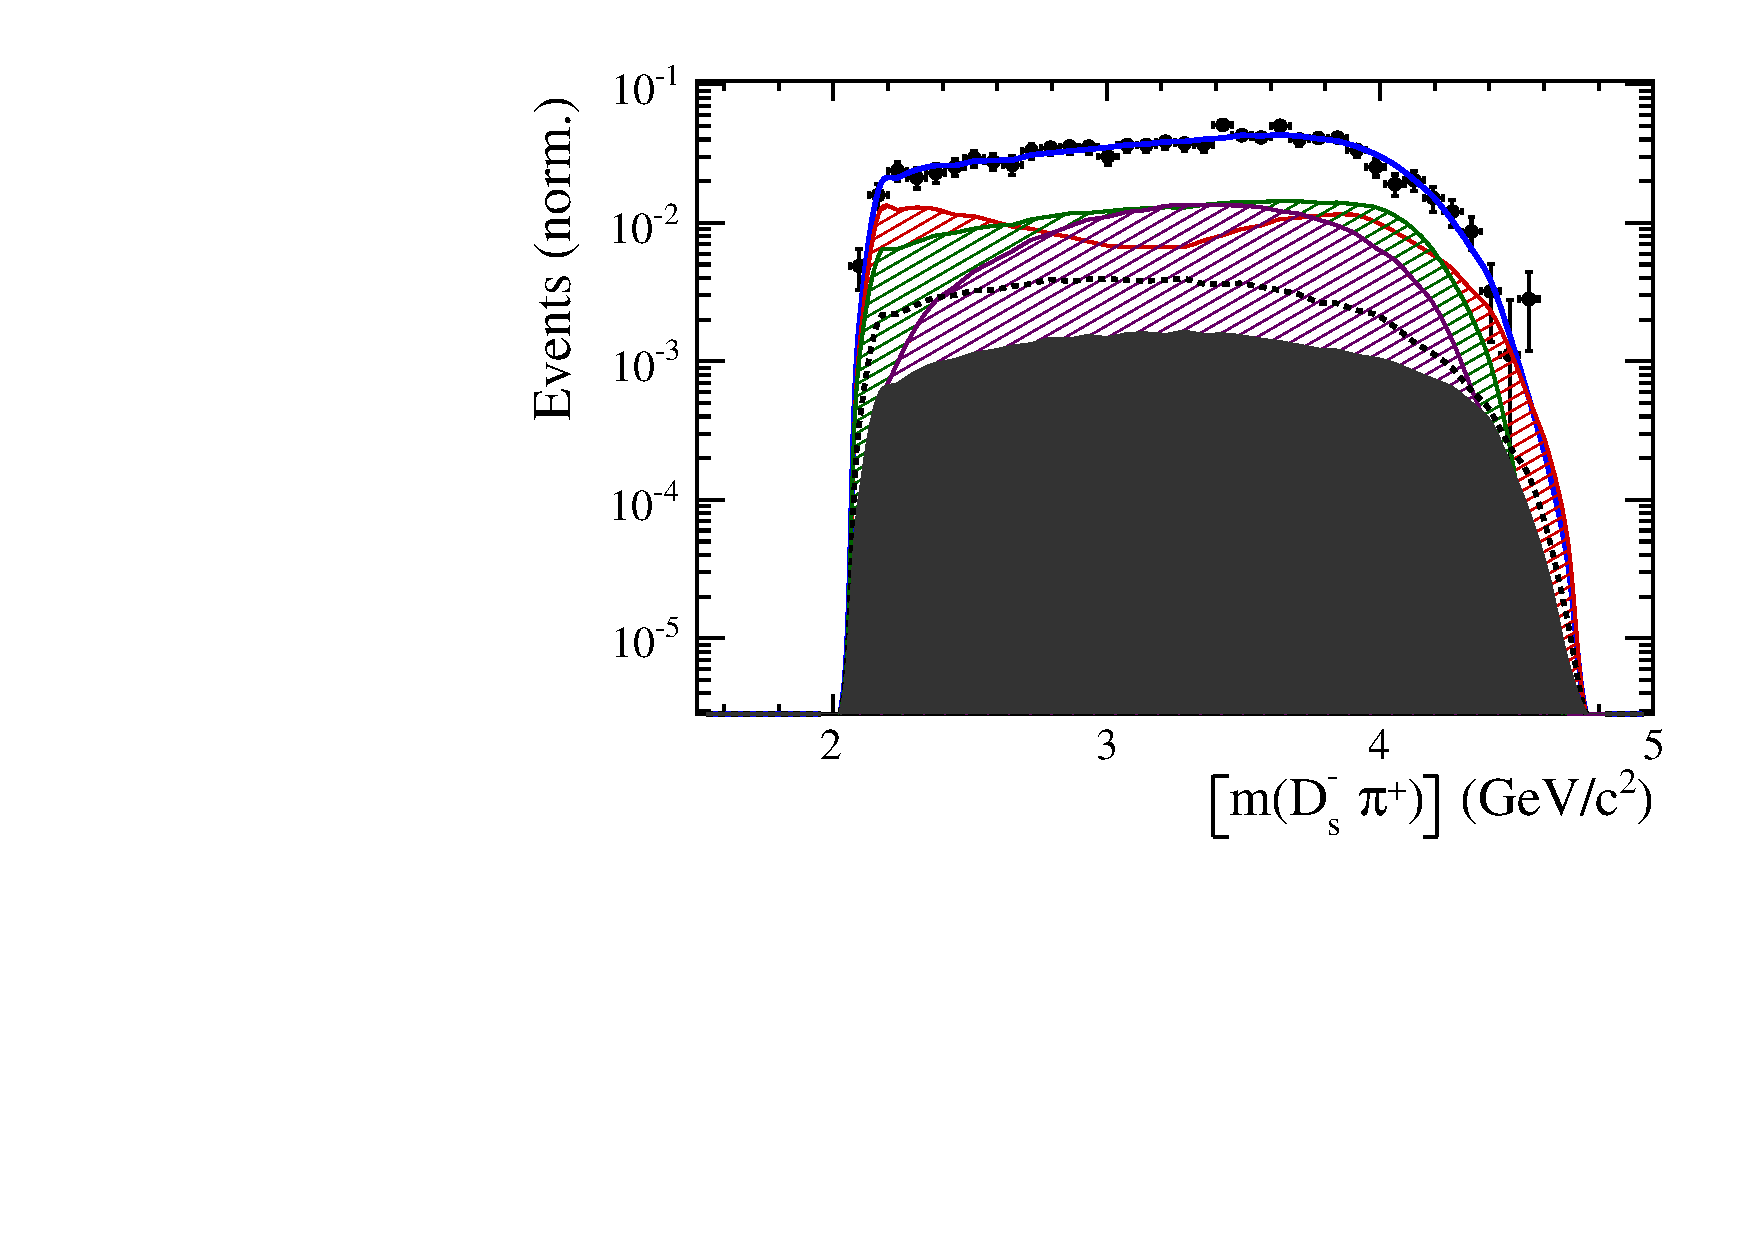
\includegraphics[width=0.32\textwidth, height = !]{figs/lassoFit/LASSO/m_Dspi_mod_log.pdf} 
		
		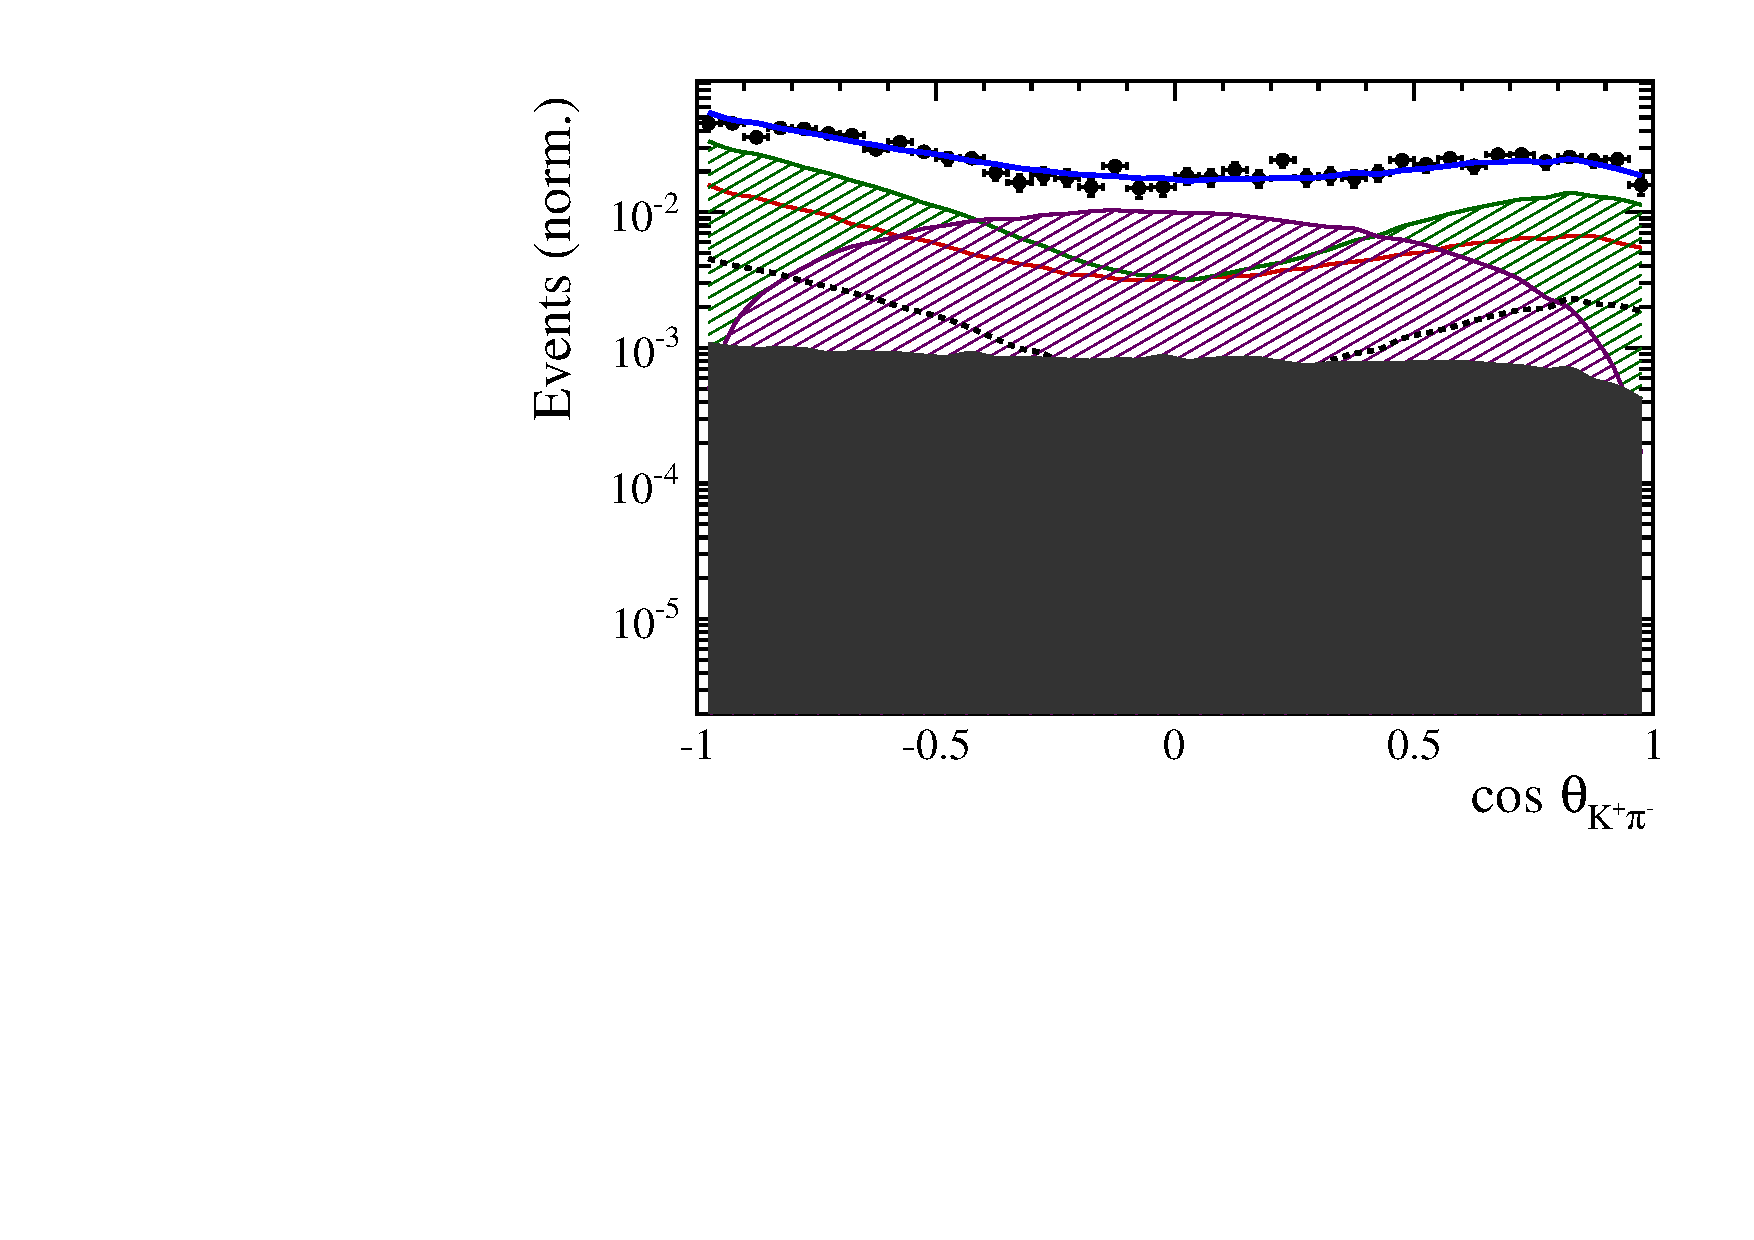
\includegraphics[width=0.32\textwidth, height = !]{figs/lassoFit/LASSO/h_cosTheta_Kpi_mod_log.pdf} 
		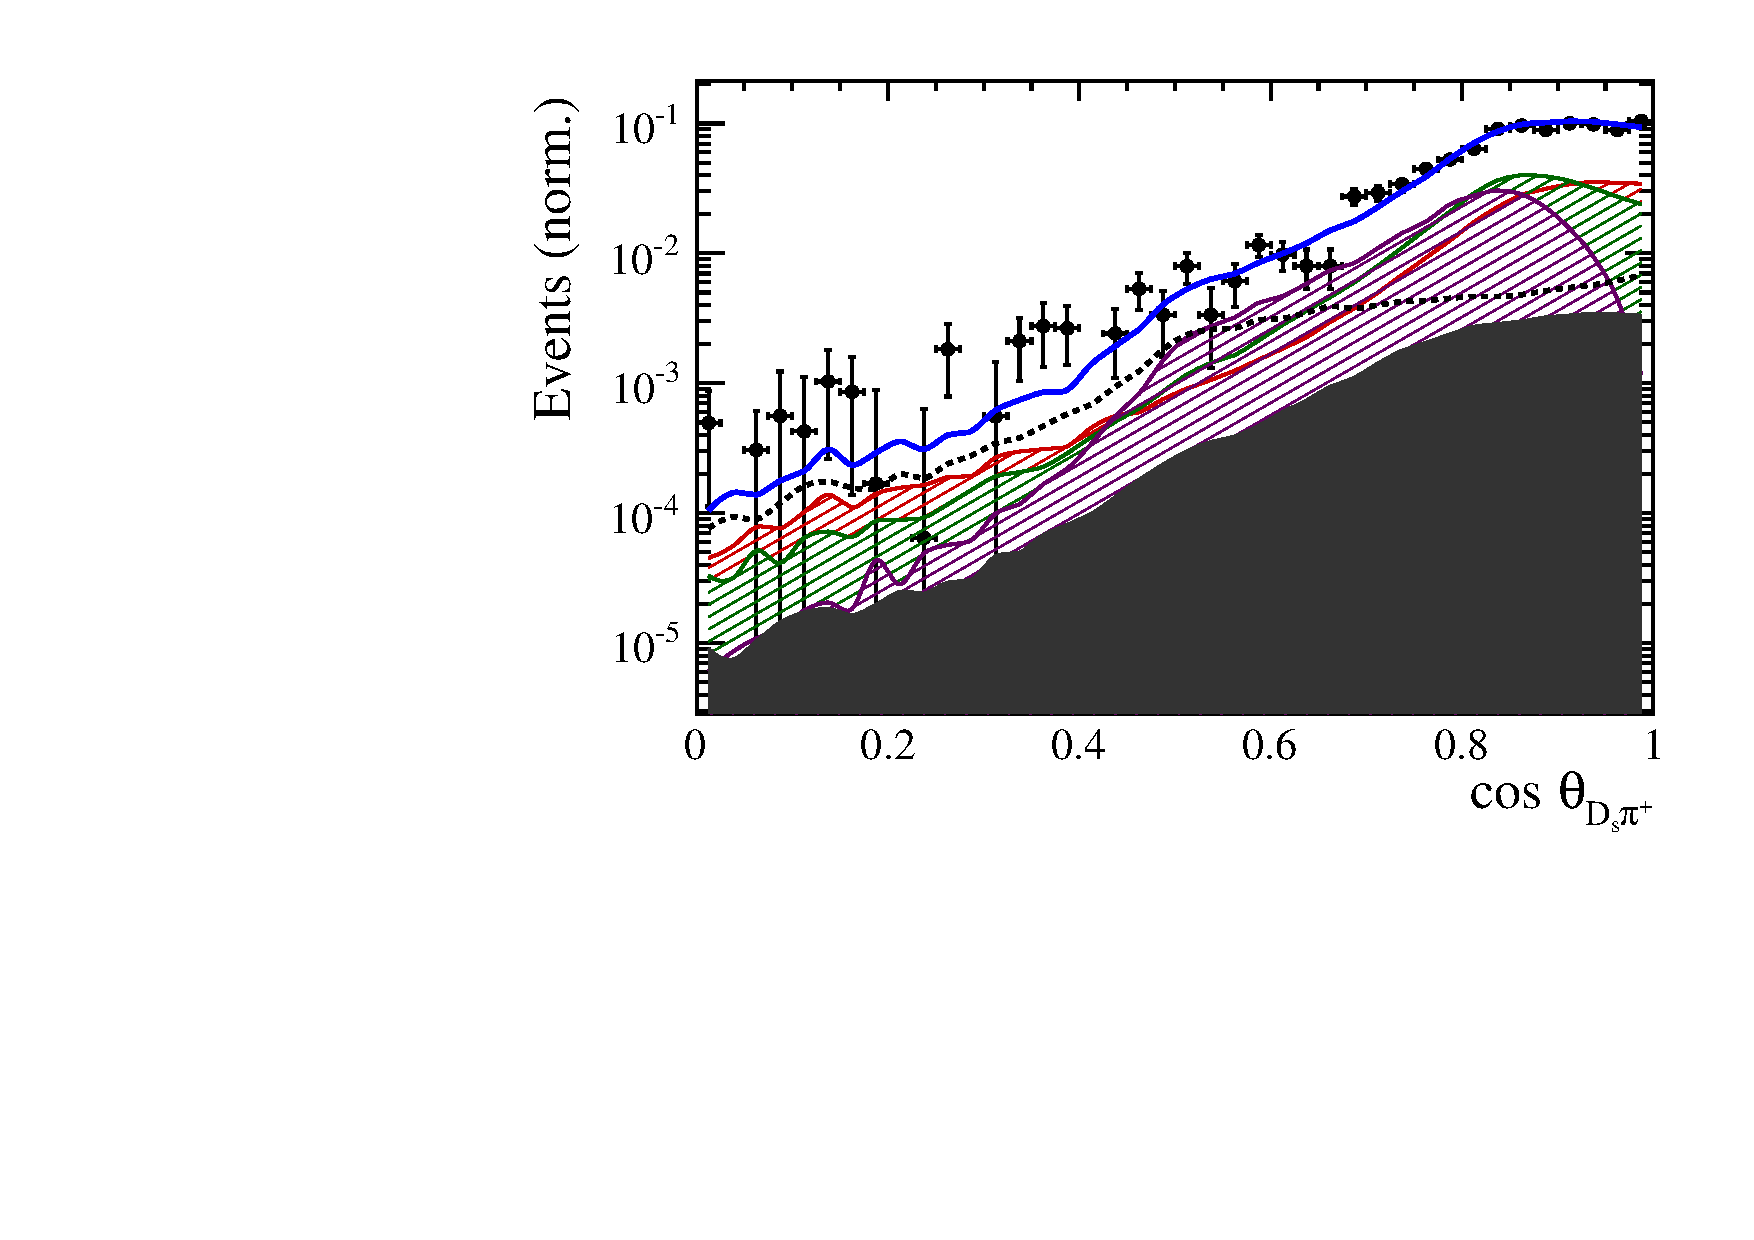
\includegraphics[width=0.32\textwidth, height = !]{figs/lassoFit/LASSO/h_cosTheta_Dspi_mod_log.pdf} 
		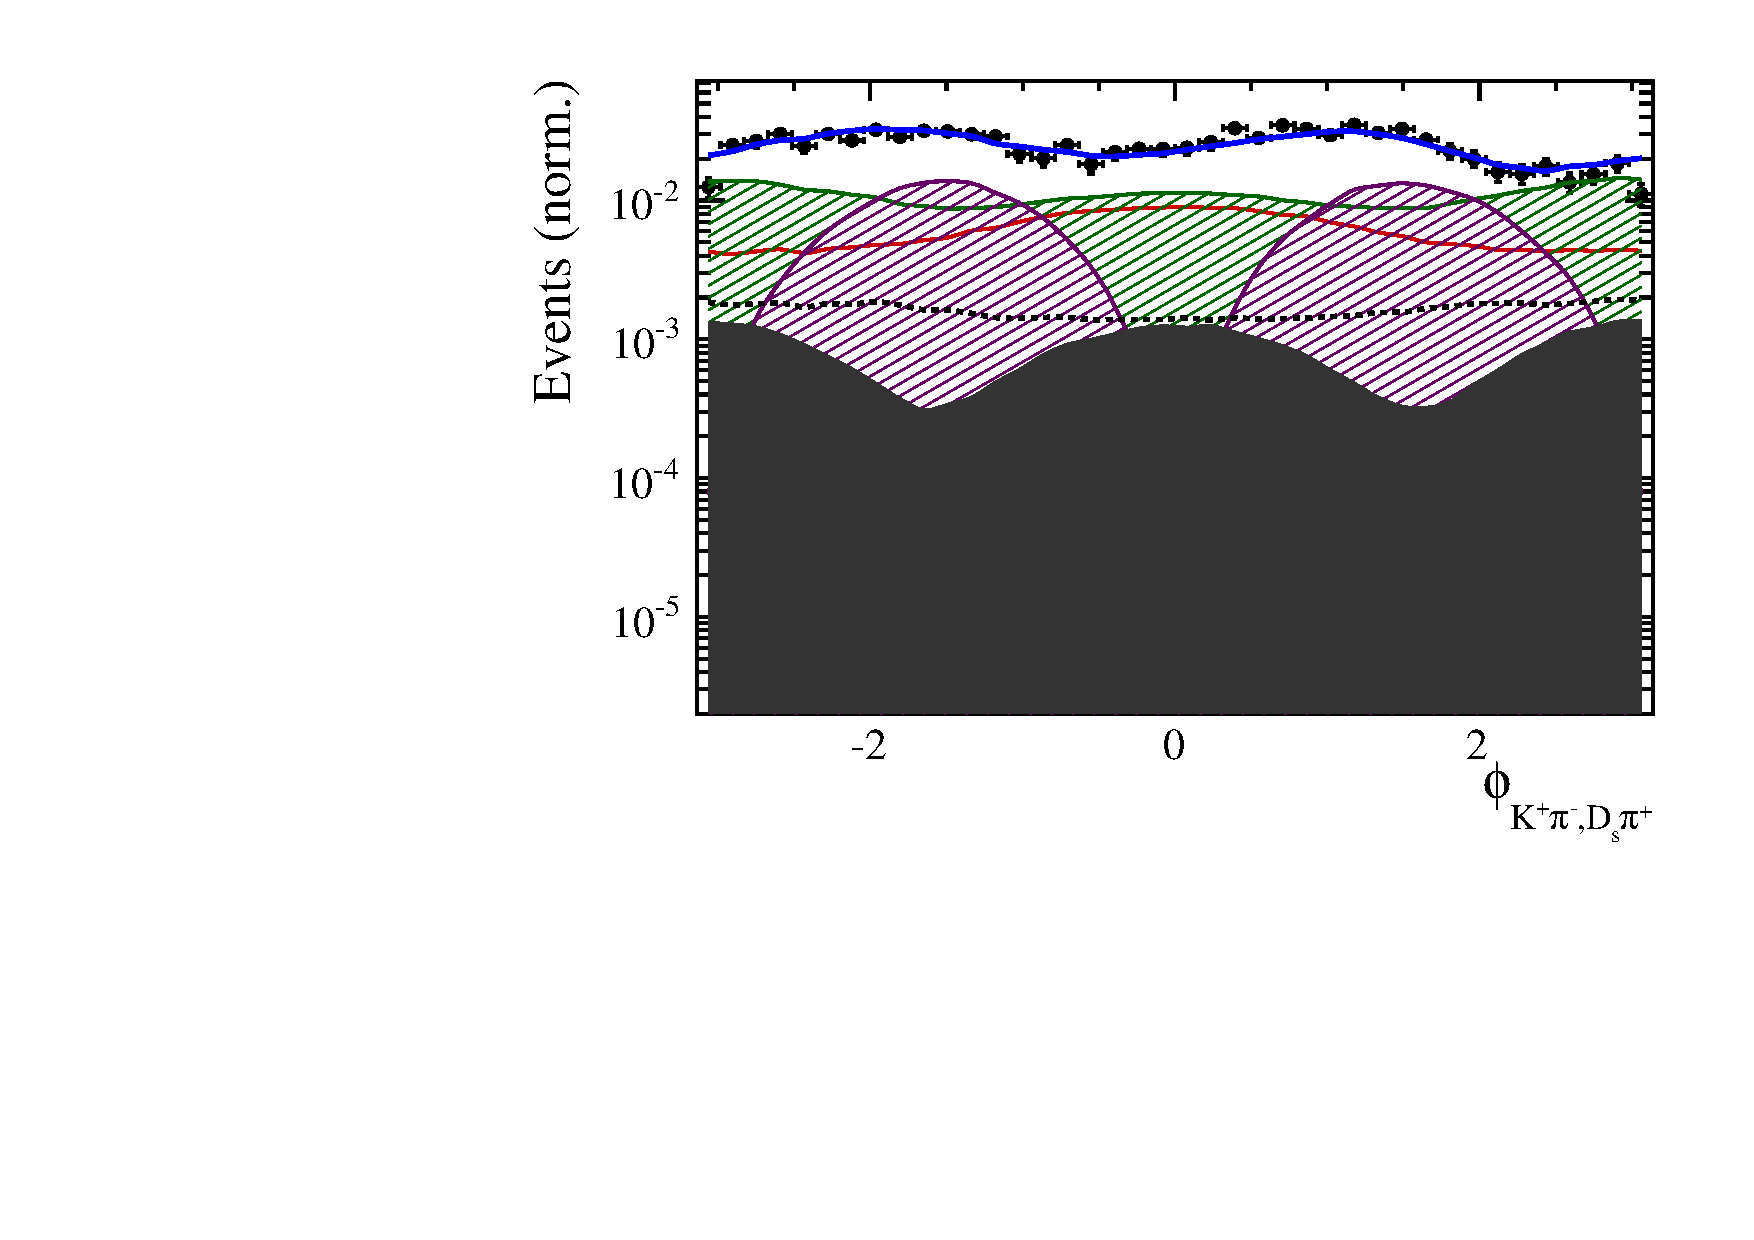
\includegraphics[width=0.32\textwidth, height = !]{figs/lassoFit/LASSO/h_phi_Kpi_Dspi_mod_log.pdf} 

		\caption{\small Projections of the fit result to the time-integrated and flavour averaged phase-space distribution of $B_s \to D_s K \pi \pi$  decays in logarithmic scale.} 		
		\label{fig:lassoFit2}
\end{figure}

\clearpage
\subsection{Results}

Table \ref{tab:fullResult} 
lists the modulus and phases of the complex amplitude coefficients $a^c_{i}$ and $a^u_{i}$, 
obtained by fitting the LASSO model to the data.
The corresponding fit fractions for the $b\to c$ and $b\to u$ amplitudes are individually normalized
\begin{equation}
\label{eq:DefineFitFractions}
	F^{c,u}_{i} \equiv \frac{\int \left\vert   a_{i}^{c,u} \, A_{i}(\phsPoint) \right\vert^{2} \, \text{d}\Phi_{4} }
	{\int \left\vert  \mathcal A_f^{c,u}(\phsPoint) \right\vert^{2} \, \text{d}\Phi_{4}}  
\end{equation}
and shown in Table \ref{tab:fullFractions}.
In addition to the amplitude coefficients, the amplitude ratio and the strong and weak phase differences between the $b\to c$ and $b\to u$ decays are determined.
Moreover, the masses and widths of the $K_1(1400)$ and $K^{*}(1410)$ resonances are fitted.

Figure \ref{fig:fullFit} shows the distributions of 
selected phase space observables, which demonstrate 
reasonable agreement between data and the fit model. 
We also project into the transversity basis to demonstrate good description of the overall angular structure.
The acoplanarity angle 
${\chi}$, is the angle between the two decay planes formed by 
the $K^+\pi^-$ system and the $D_s^- \pip$ system
in the $B_s$ rest frame; boosting into the rest frames of the two-body systems defining these decay planes,
the two helicity variables 
are defined as the cosine of the angle, ${\theta}$, 
of the $K^+$ or $D_S^-$ momentum with the $B_s$ flight direction.

In order to quantify the quality of the fit in the five-dimensional phase space,
a \chisq value is determined by binning the data;
\begin{equation}
	\chi^{2} = \sum_{b=1}^{N_{\rm bins}} \frac{(N_{b}-N_{b}^{\rm exp})^{2}}{N_{b}^{\rm exp}},
\end{equation}
where $N_{b}$ is the number of data events in a given bin, 
$N_{b}^{\rm exp}$ is the event count predicted by the fitted PDF
and $N_{\rm bins}$ is the number of bins.
%The phase space is binned in terms of $min$
An adaptive binning
is used to ensure sufficient statistics in each bin for a robust $\chi^{2}$ calculation ~\cite{KKpipi}.
At least $25$ events per bin are required.
The number of degrees of freedom $\nu$, in an unbinned fit is bounded by $N_{\rm bins}-1$ and $(N_{\rm bins}- 1) - N_{\rm par}$, 
where $N_{\rm par}$ is the number of free fit parameters.
We use the \chisq value divided by $\nu = (N_{\rm bins}-1) - N_{\rm par}$ as a conservative estimate.
For the LASSO model, this 
amounts to $\chisq/\nu = 1.40$ %with $\nu = 221$,
indicating a decent fit quality.

\begin{table}[h]
\centering
\caption{
\small
Modulus and phases of the amplitudes contributing to $b \to c$ and $b \to u$ decays.
In case of multiple decay modes of three-body resonances, the amplitude coefficients are defined relative to the one listed first.
Additional fit parameters are listed below.
The first quoted uncertainty is statistical, while the second arises from systematic sources. 
The third uncertainty arises from the alternative models considered.
}
\resizebox{\linewidth}{!}{
	\renewcommand{\arraystretch}{1.5}
	\begin{tabular}{l c c c c } 
\hline
\hline
\multicolumn{1}{c}{Decay Channel} & \multicolumn{2}{c}{$A_{b \to c}$} & \multicolumn{2}{c}{$A_{b \to u}$}  \\ 
 & \multicolumn{1}{c}{$\vert a_i \vert$}  & \multicolumn{1}{c}{$arg(a_i) [\degrees]$}  & \multicolumn{1}{c}{$\vert a_i \vert$} & \multicolumn{1}{c}{$arg(a_i) [\degrees]$} \\ 
\hline
 $B_s \to D_s \, ( K_1(1270) \to K \, \rho(770) ) $ &  1.0 & 0.0 & 1.0 & 0.0  \\ 
$\phantom{B_s \to D_s \, (} K_1(1270) \to K^{*}(892) \, \pi \phantom{)} $ & 0.76 $\pm$ 0.11 $\pm$ 0.16 & 60.9 $\pm$ 9.6 $\pm$ 14.0 & &   \\ 
$\phantom{B_s \to D_s \, (} K_1(1270) \to K^{*}_{0}(1430) \, \pi \phantom{)} $ & 0.68 $\pm$ 0.06 $\pm$ 0.34 & 116.5 $\pm$ 5.1 $\pm$ 43.5 & &   \\ 
$B_s \to D_s \, ( K_1(1400) \to K^{*}(892) \, \pi ) $ & 2.53 $\pm$ 0.27 $\pm$ 0.57 & 12.9 $\pm$ 7.4 $\pm$ 8.0 & 0.67 $\pm$ 0.20 $\pm$ 0.51 & -76.3 $\pm$ 16.9 $\pm$ 22.8 \\ 
$B_s \to D_s \, ( K^{*}(1410) \to K^{*}(892) \, \pi ) $ & 1.28 $\pm$ 0.12 $\pm$ 0.24 & 54.9 $\pm$ 5.6 $\pm$ 9.8 &  &  \\ 
$\phantom{B_s \to D_s \, (} K^{*}(1410) \to K \, \rho(770) \phantom{)} $ & 0.66 $\pm$ 0.04 $\pm$ 0.03 & -172.9 $\pm$ 5.0 $\pm$ 6.5 & &   \\ 
$B_s \to D_s \, ( K(1460) \to K^{*}(892) \, \pi ) $ & & &0.77 $\pm$ 0.11 $\pm$ 0.62 & -93.6 $\pm$ 11.2 $\pm$ 12.1 \\ 
$B_s \to ( D_s \, \pi)_{P} \, \, K^{*}(892) $ & 1.02 $\pm$ 0.13 $\pm$ 0.41 & -28.4 $\pm$ 8.0 $\pm$ 10.4 & 0.79 $\pm$ 0.18 $\pm$ 0.35 & 3.7 $\pm$ 12.5 $\pm$ 14.8 \\ 
$B_s \to ( D_s \, K)_{P} \, \, \rho(770) $ & & &0.61 $\pm$ 0.08 $\pm$ 0.26 & 36.4 $\pm$ 7.7 $\pm$ 14.1 \\ 
\hline
\hline
\multicolumn{1}{c}{Fit parameter} & \multicolumn{4}{c}{Value}  \\ 
\hline
\multicolumn{1}{c}{$m_{K_1(1400)} \, [\text{MeV}]$} & \multicolumn{4}{c}{1394.9 $\pm$ 8.8 $\pm$ 12.6 $\pm$ 21.2} \\ 
\multicolumn{1}{c}{$\Gamma_{K_1(1400)} \, [\text{MeV}]$} & \multicolumn{4}{c}{224.0 $\pm$ 15.9 $\pm$ 22.0 $\pm$ 20.9} \\ 
\multicolumn{1}{c}{$m_{K^{*}(1410)} \, [\text{MeV}]$} & \multicolumn{4}{c}{1419.6 $\pm$ 10.8 $\pm$ 26.8 $\pm$ 24.1} \\ 
\multicolumn{1}{c}{$\Gamma_{K^{*}(1410)} \, [\text{MeV}]$} & \multicolumn{4}{c}{342.4 $\pm$ 23.5 $\pm$ 51.0 $\pm$ 52.9} \\ 
 \\ 
\multicolumn{1}{c}{$r$} & \multicolumn{4}{c}{xx.xx $\pm$ 0.04 $\pm$ 0.05 $\pm$ 0.04} \\ 
\multicolumn{1}{c}{$\delta \, [\degrees]$} & \multicolumn{4}{c}{xx.xx $\pm$ 16.1 $\pm$ 6.2 $\pm$ 6.8} \\ 
\multicolumn{1}{c}{$\gamma - 2 \beta_{s} \, [\degrees]$} & \multicolumn{4}{c}{xx.xx $\pm$ 16.1 $\pm$ 11.4 $\pm$ 6.2} \\ 
\hline
\hline
\end{tabular}

}
\label{tab:fullResult}
\end{table}

\clearpage

\begin{figure}[h]
	\centering
		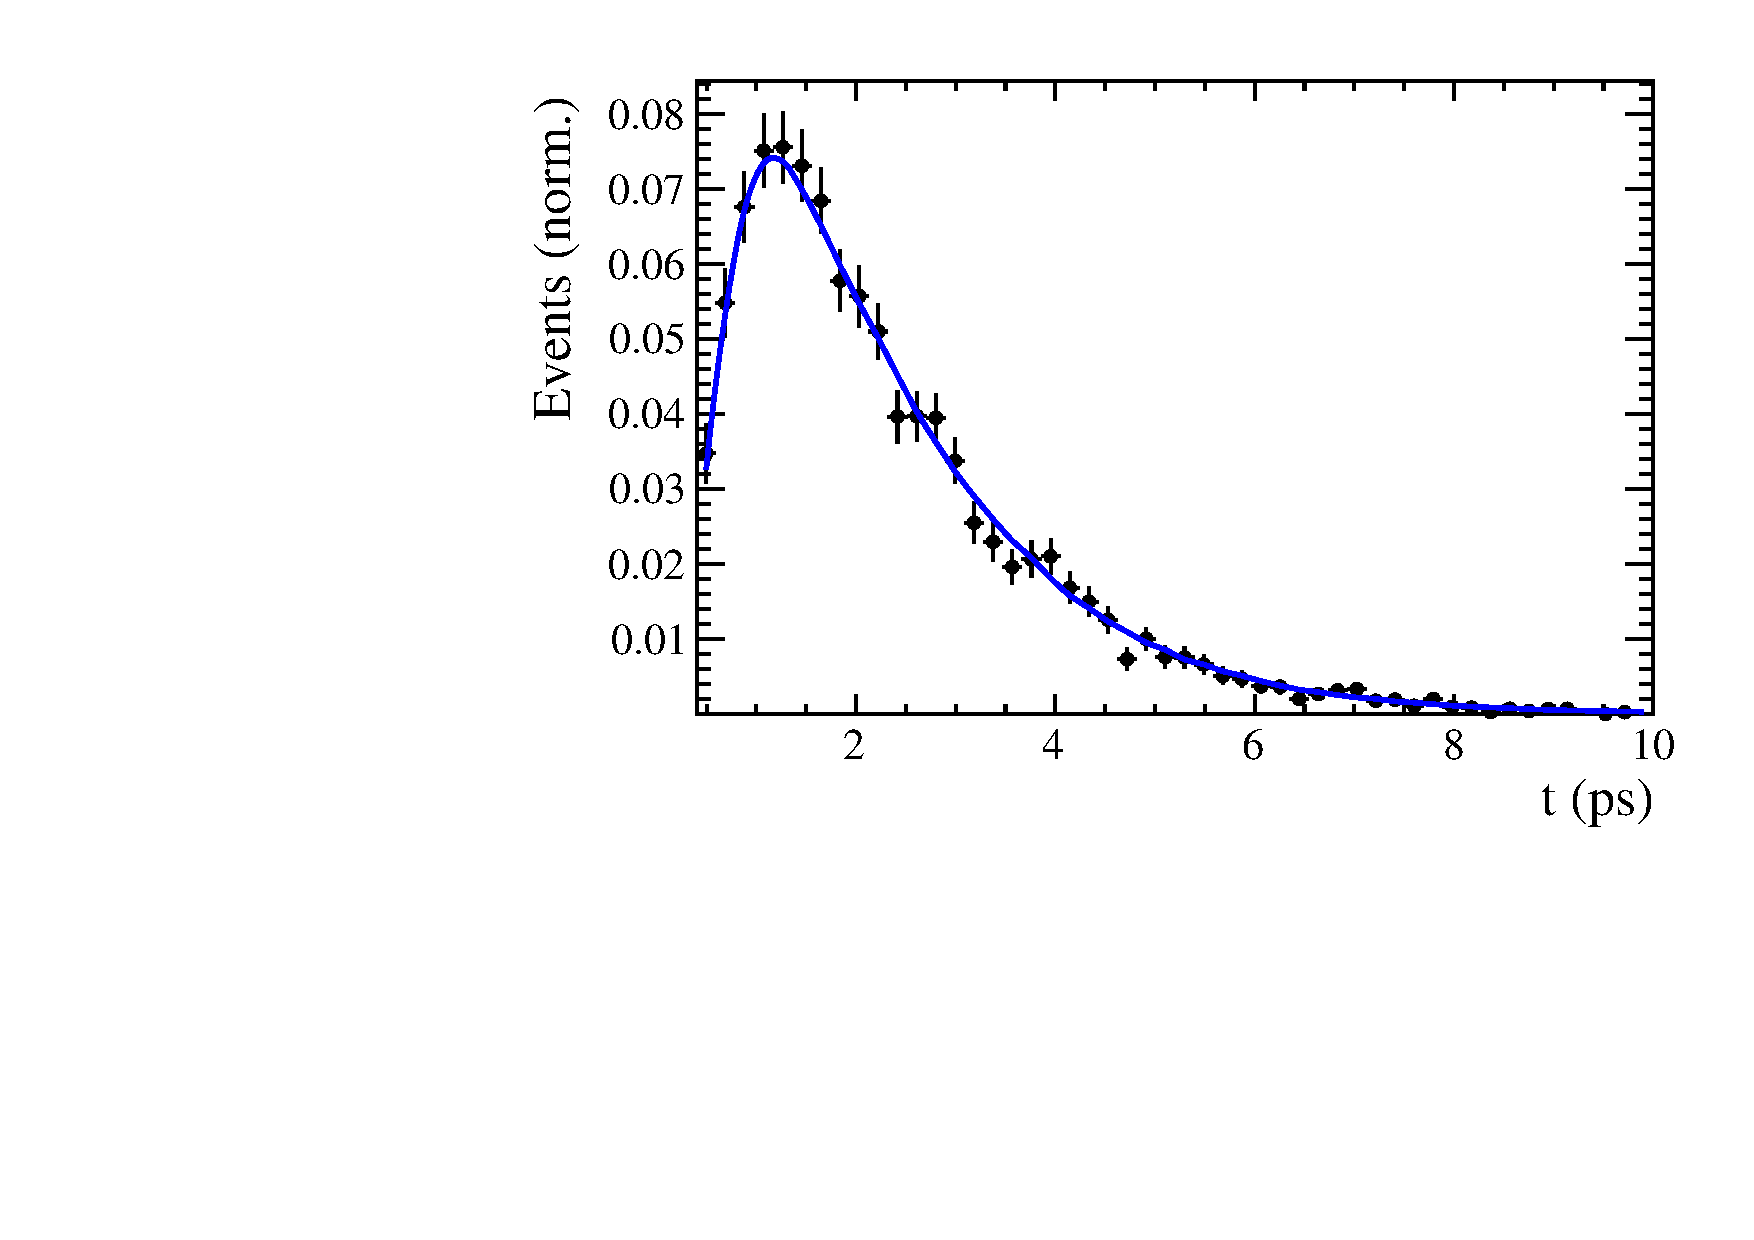
\includegraphics[width=0.3\textwidth, height = !]{figs/fullFit/signal/h_t.pdf} 
		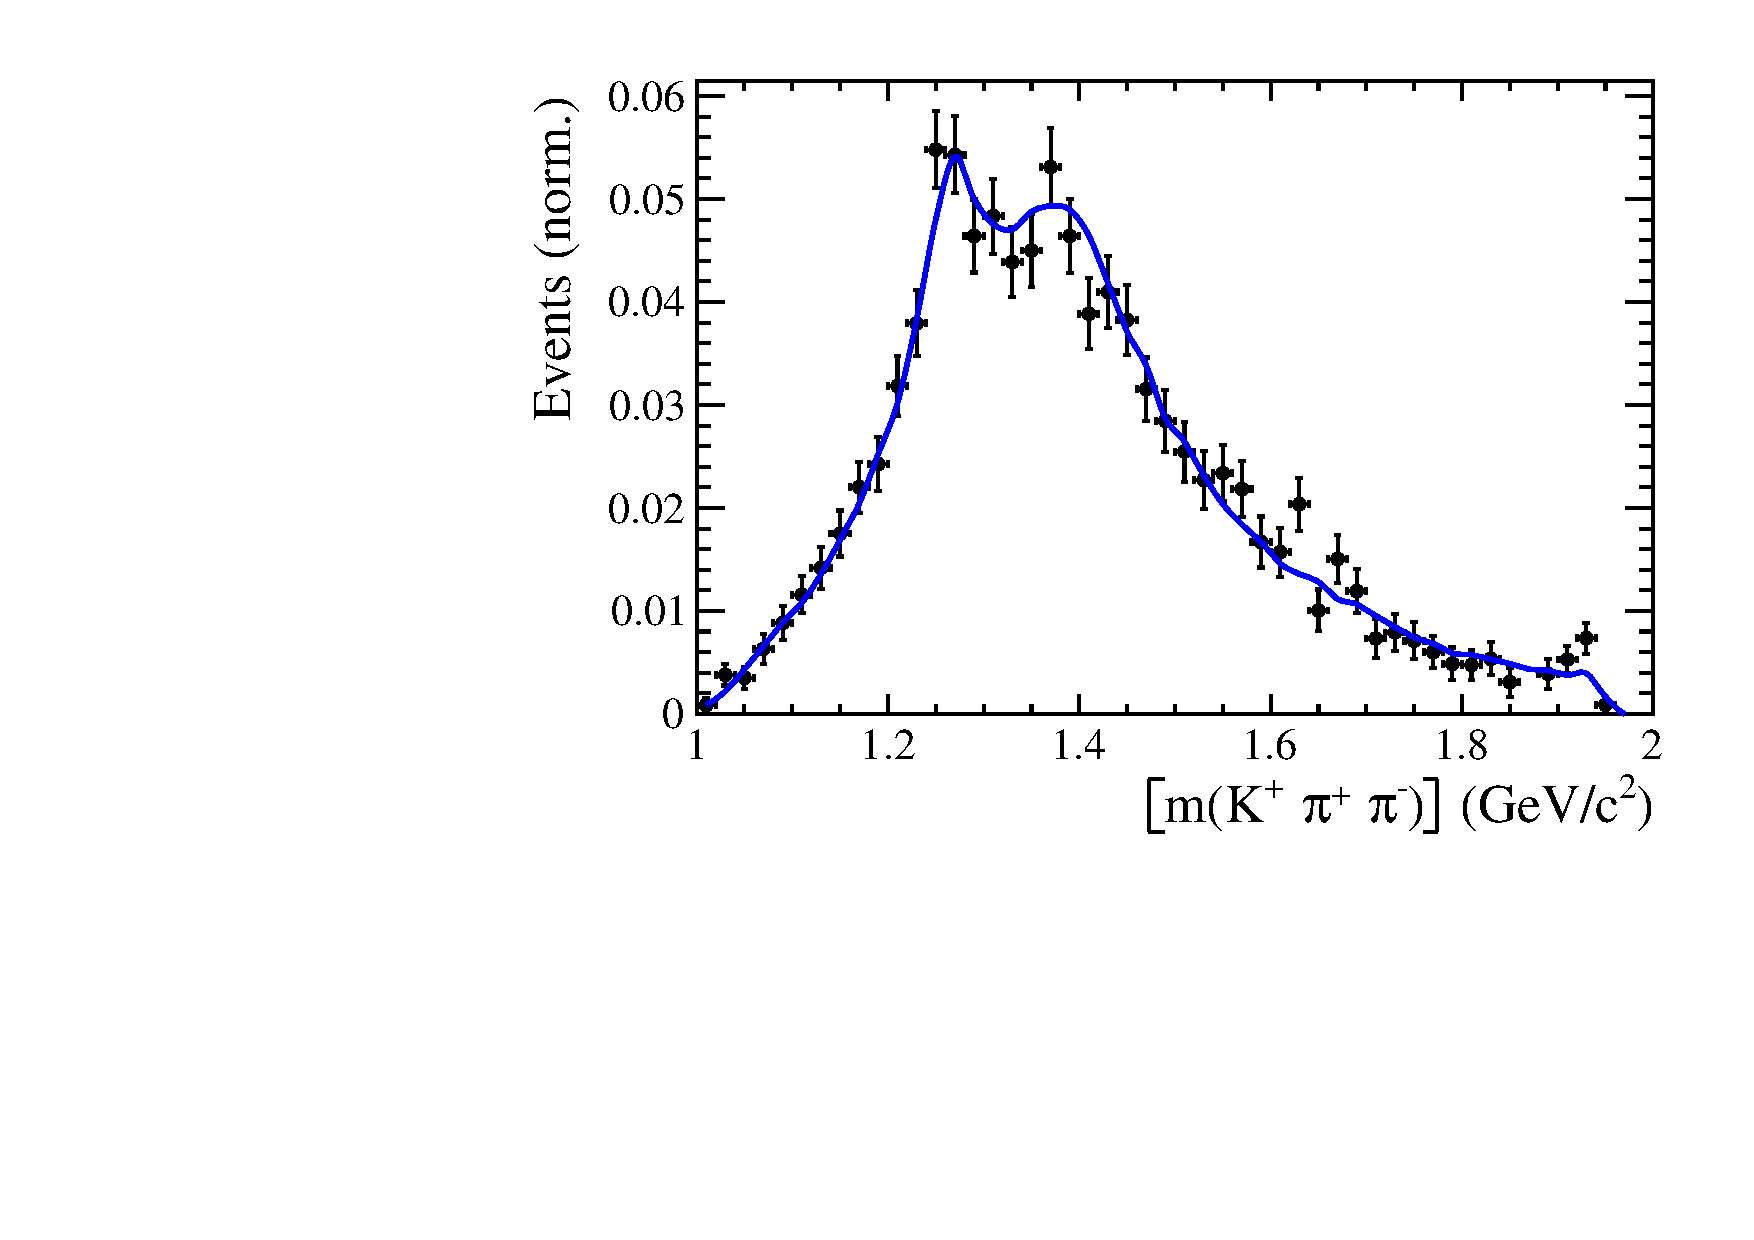
\includegraphics[width=0.3\textwidth, height = !]{figs/fullFit/signal/m_Kpipi.pdf} 
		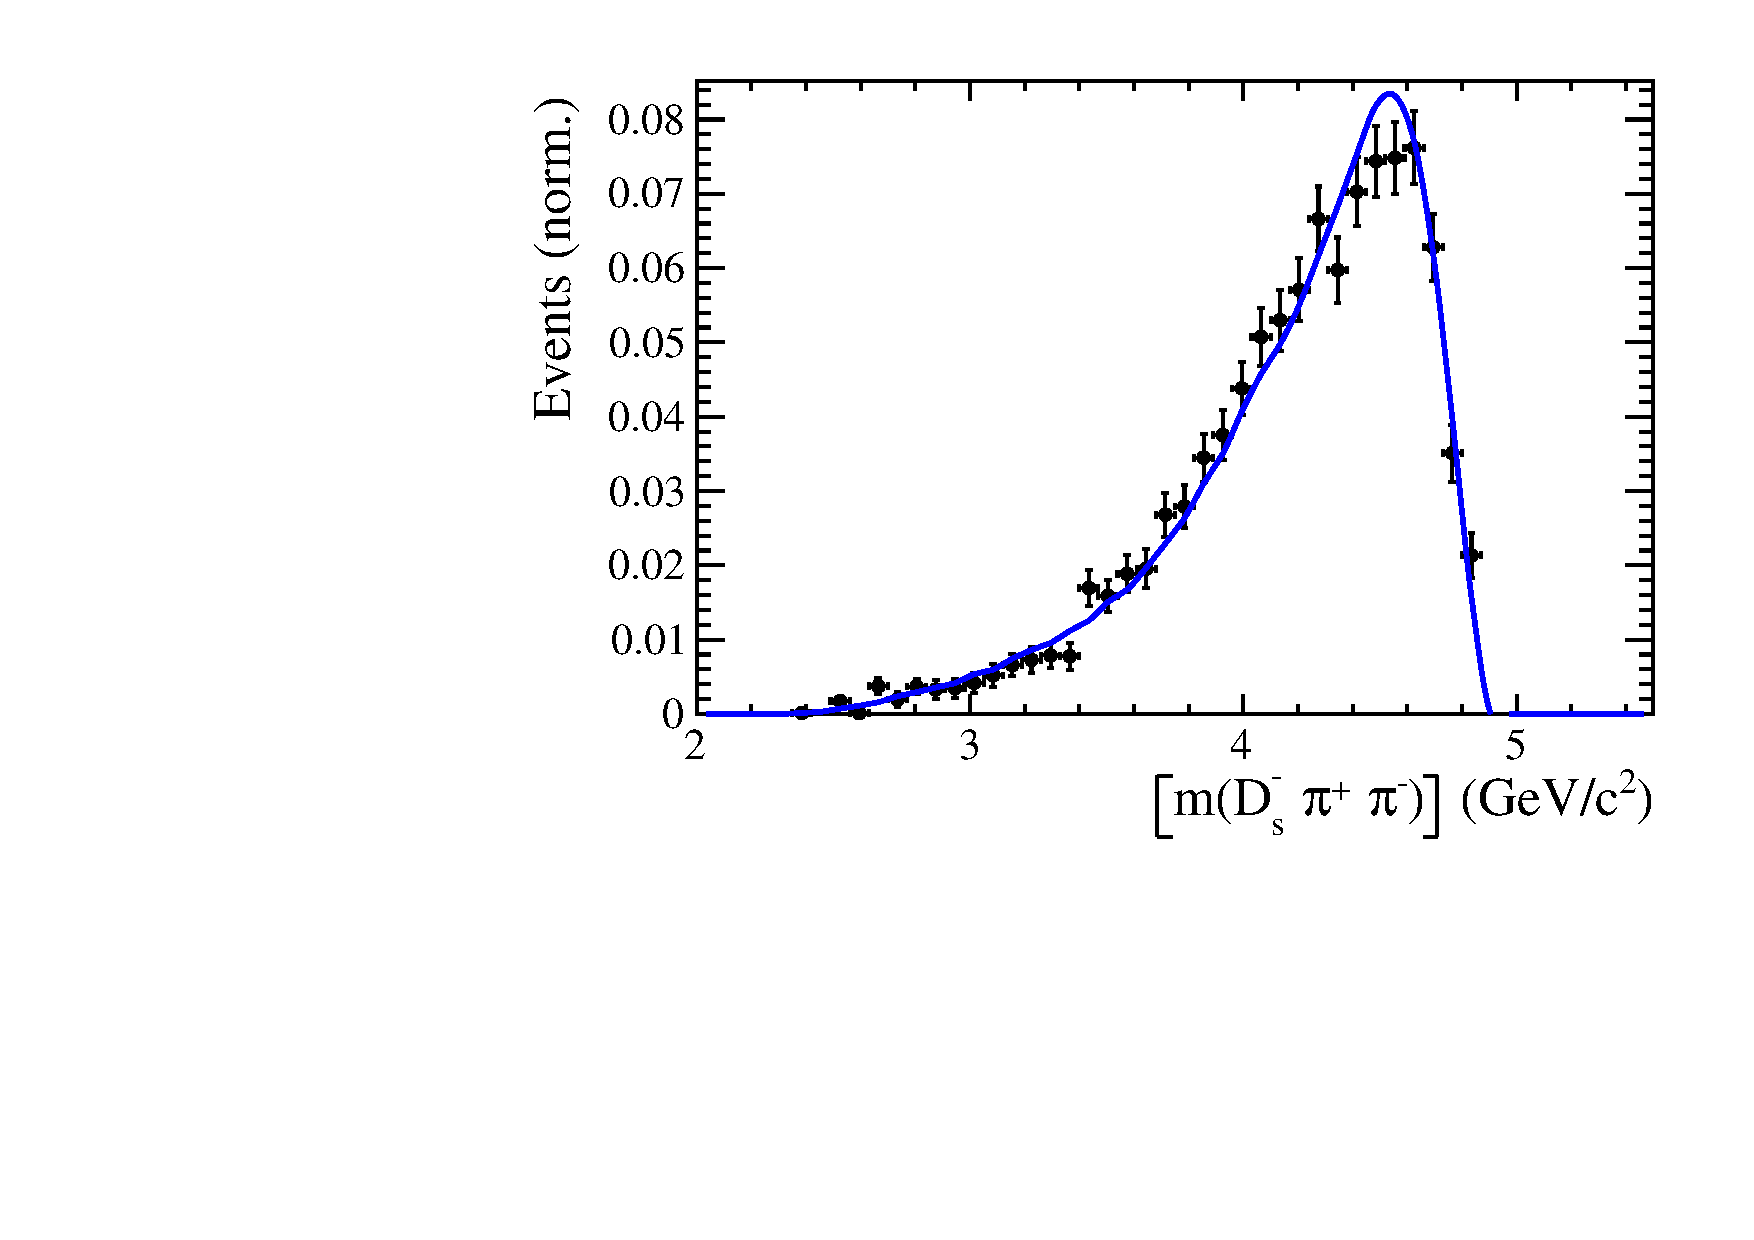
\includegraphics[width=0.3\textwidth, height = !]{figs/fullFit/signal/m_Dspipi.pdf} 

		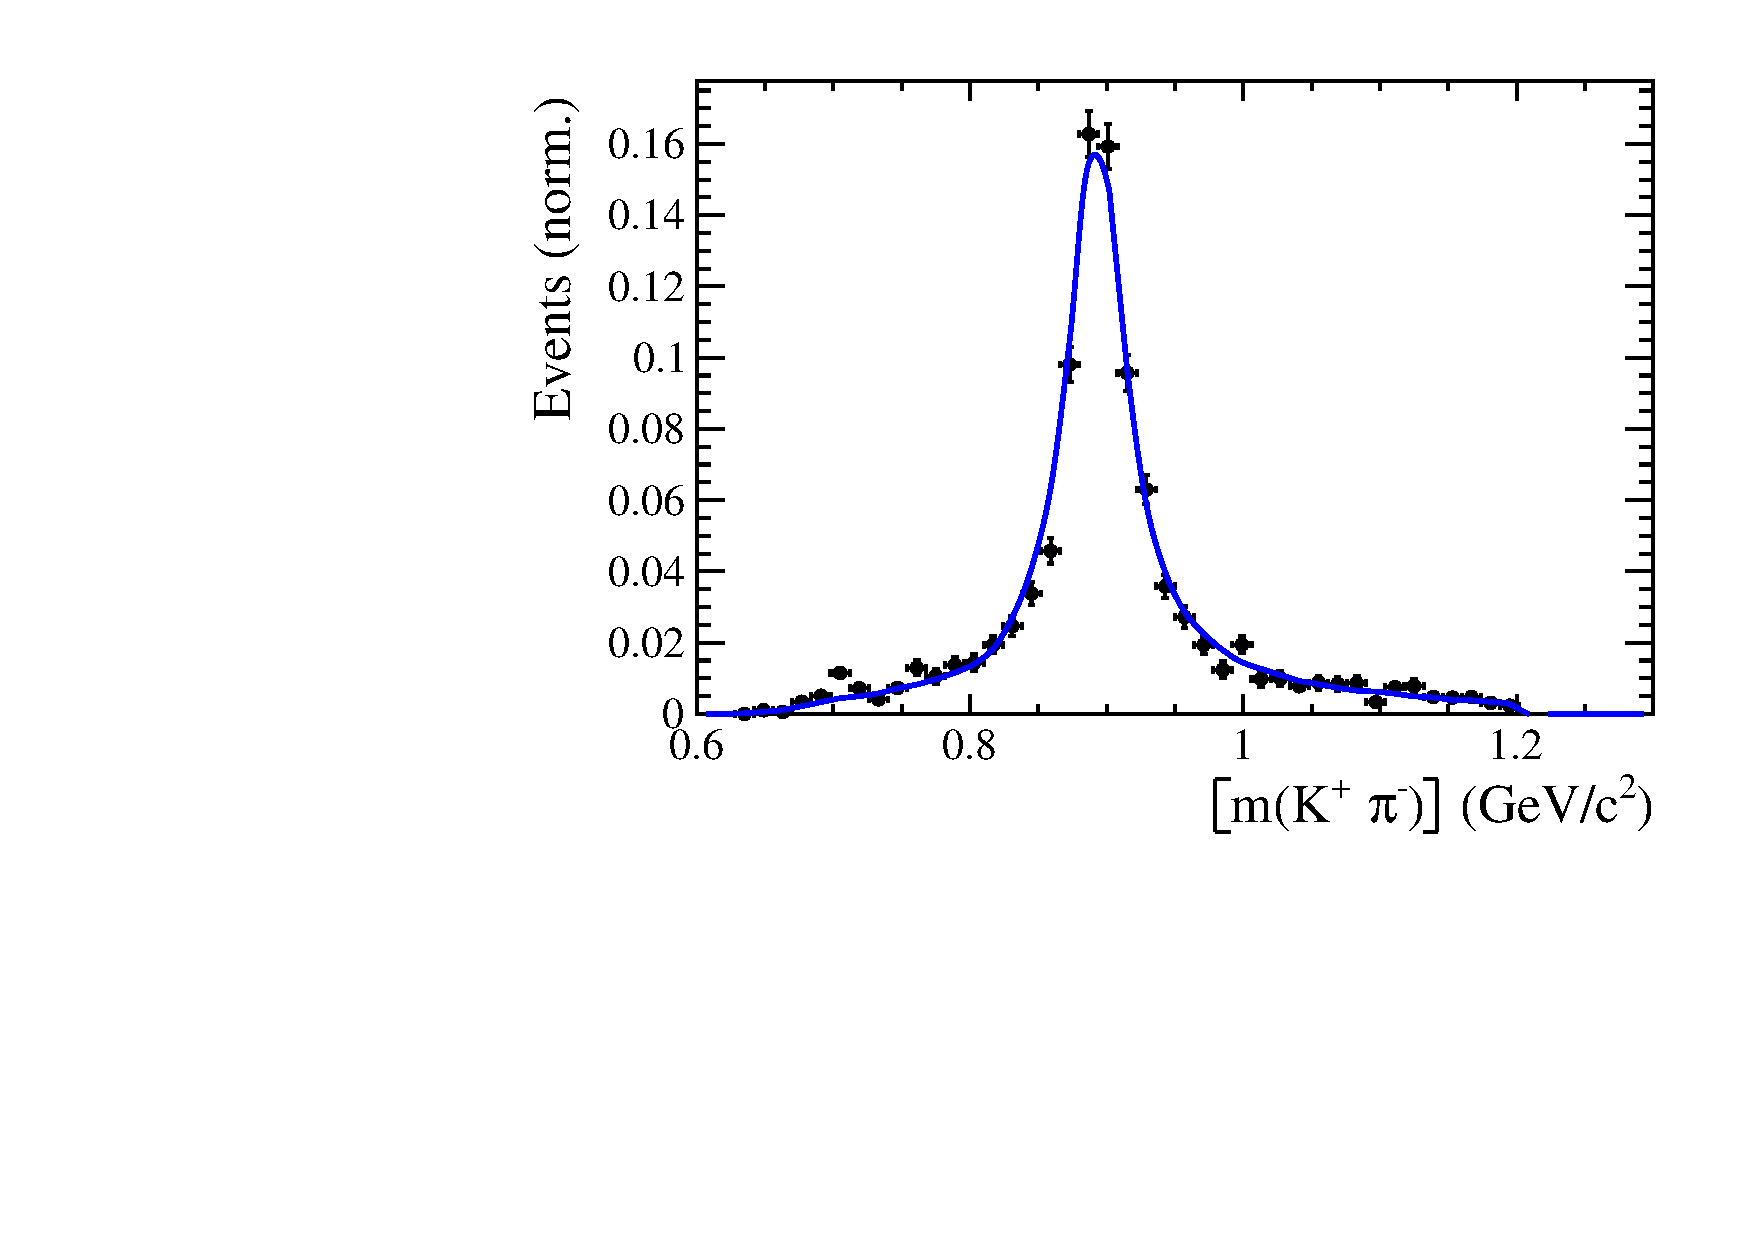
\includegraphics[width=0.3\textwidth, height = !]{figs/fullFit/signal/m_Kpi.pdf} 
		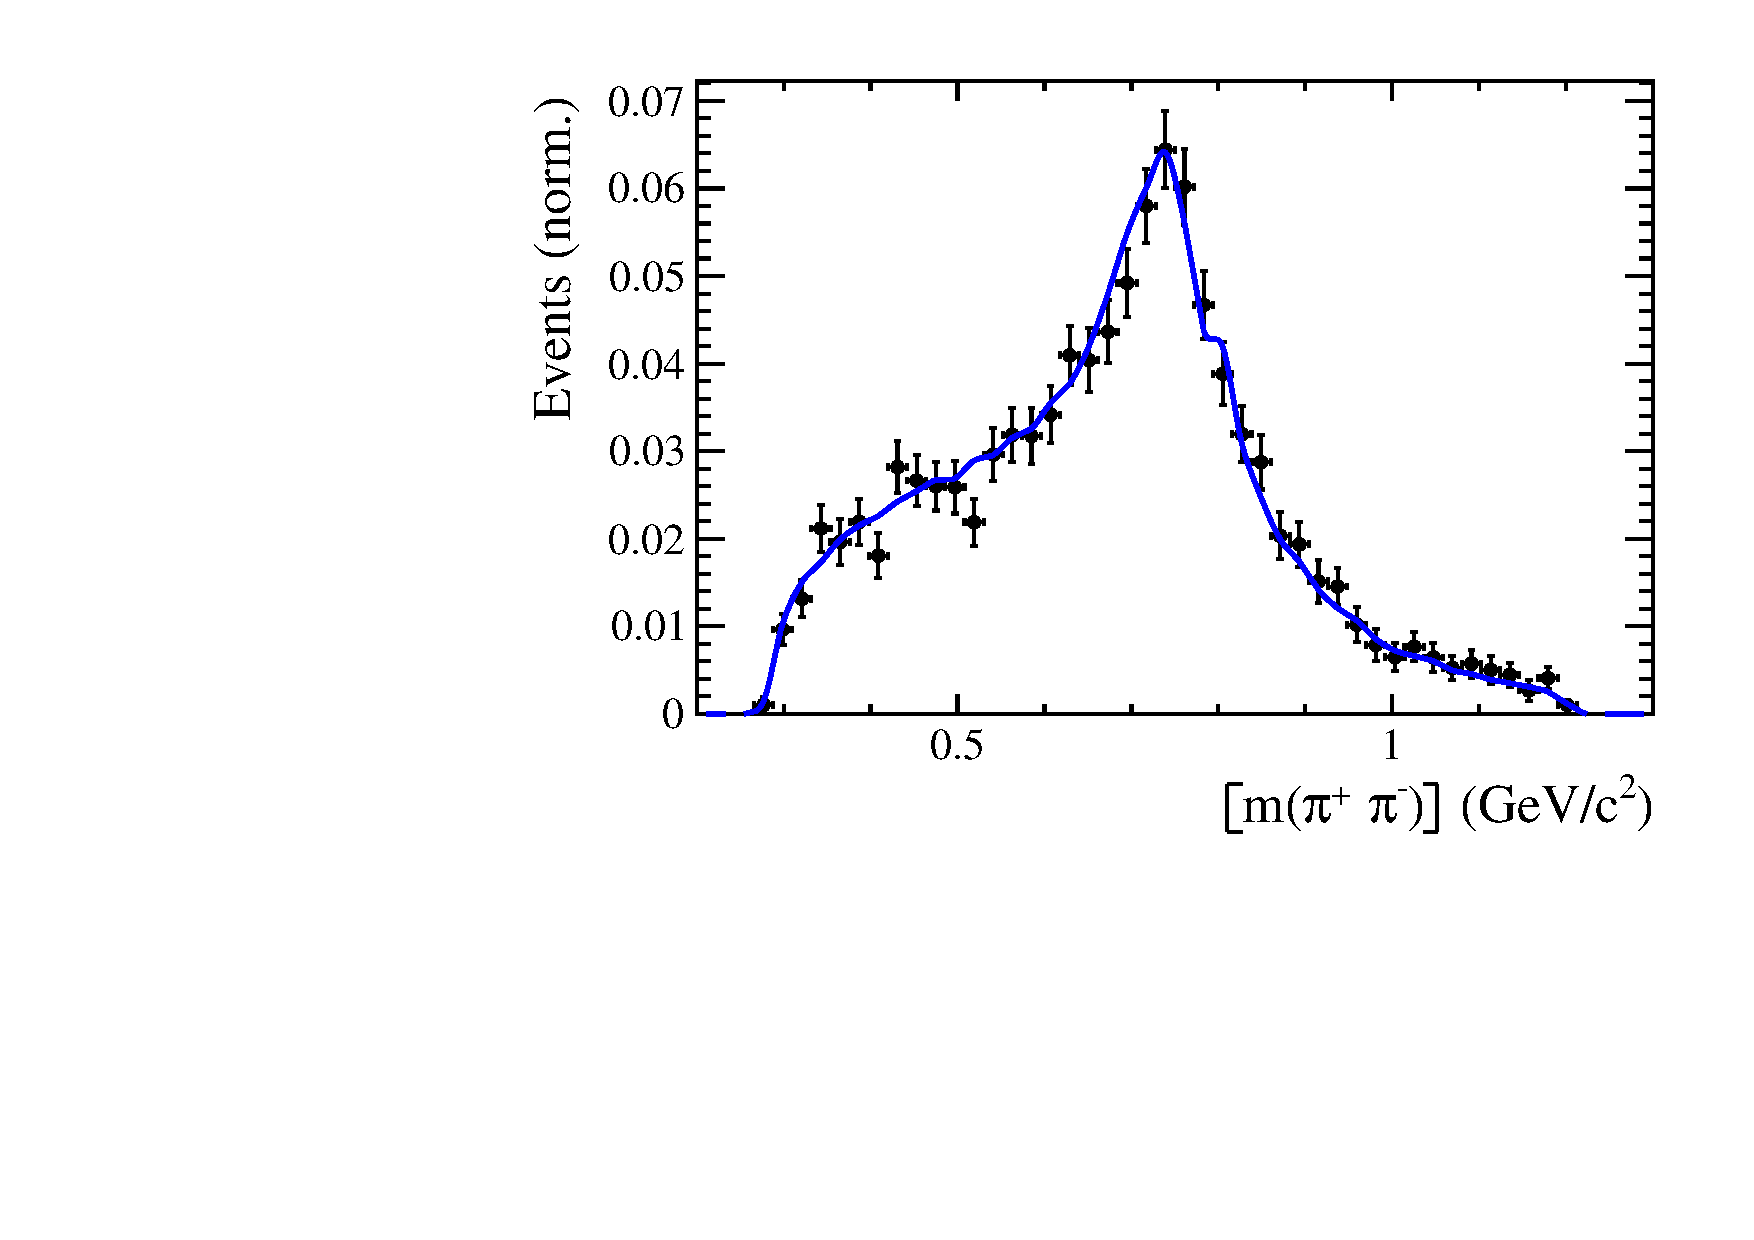
\includegraphics[width=0.3\textwidth, height = !]{figs/fullFit/signal/m_pipi.pdf} 
		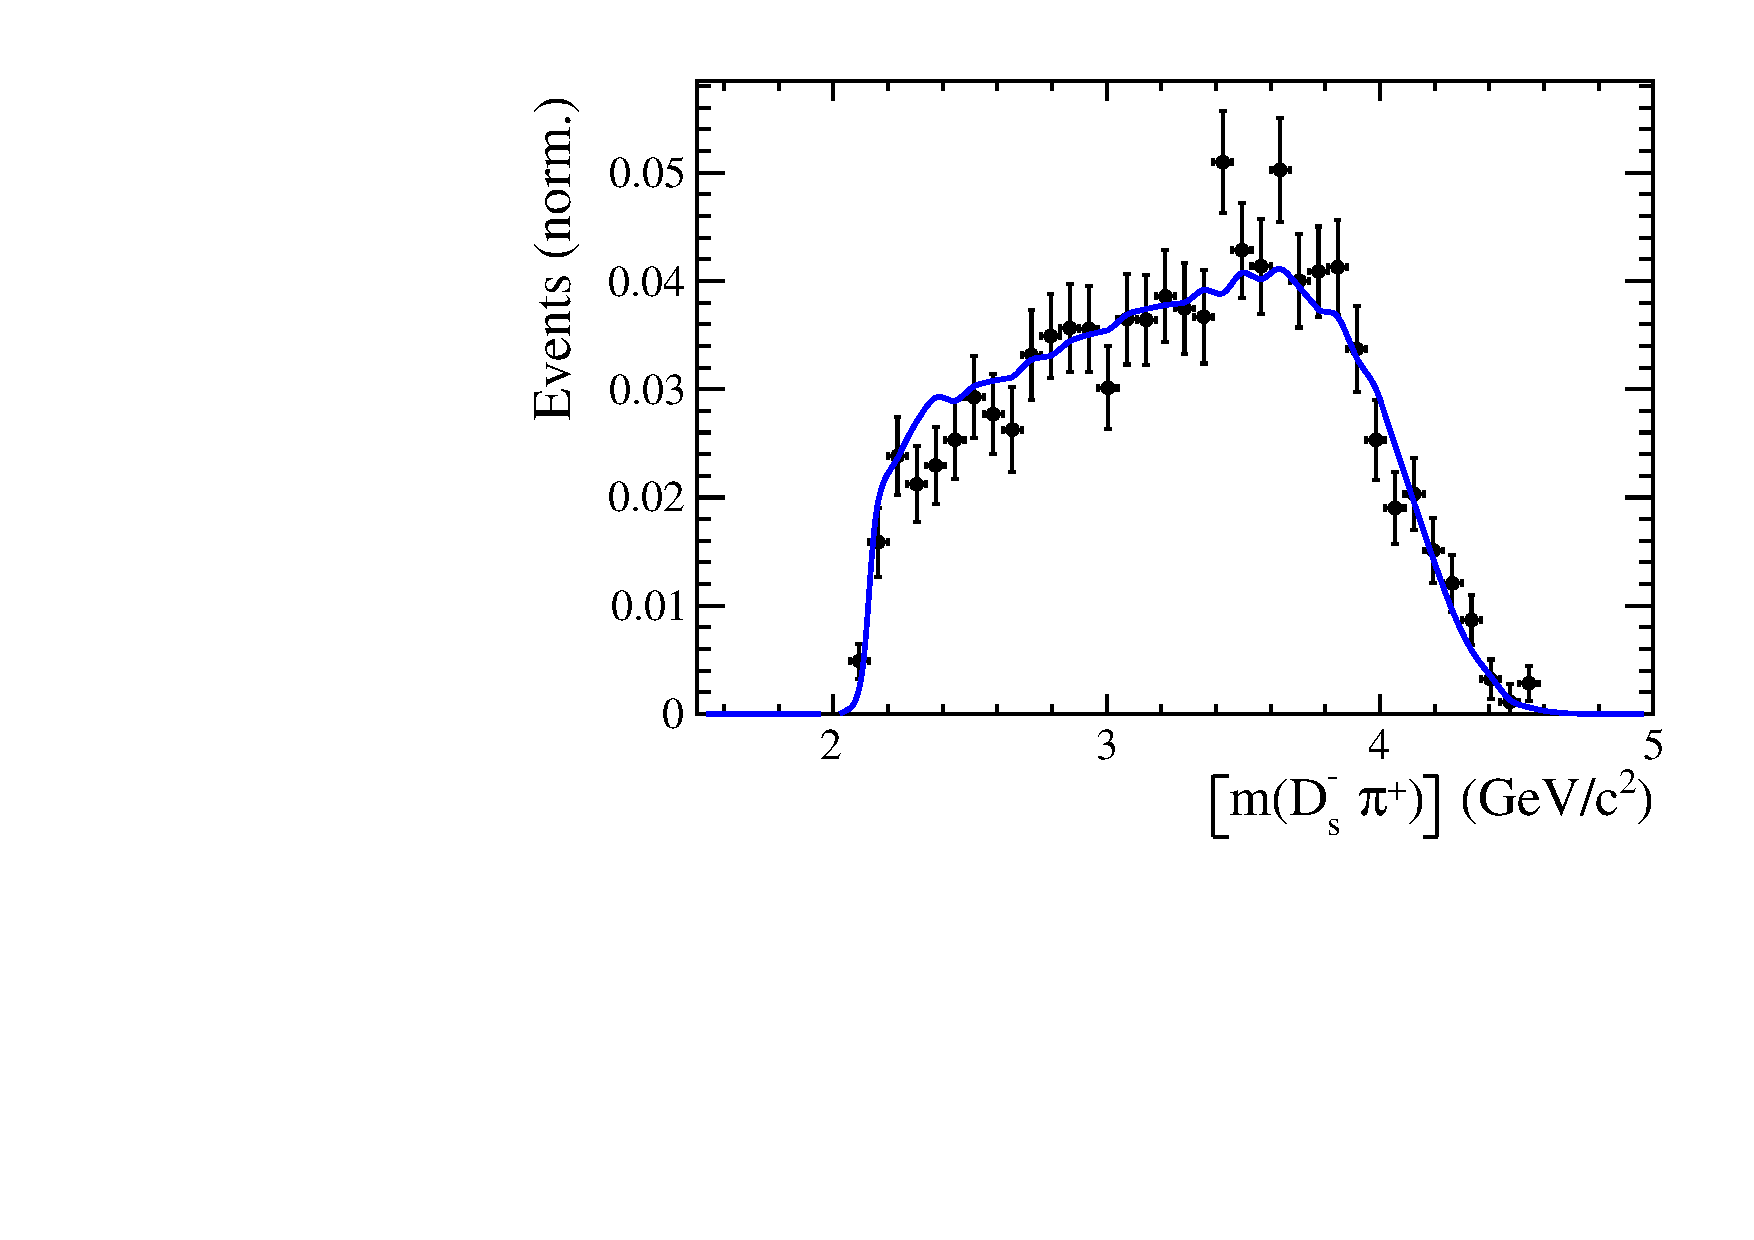
\includegraphics[width=0.3\textwidth, height = !]{figs/fullFit/signal/m_Dspi.pdf} 

		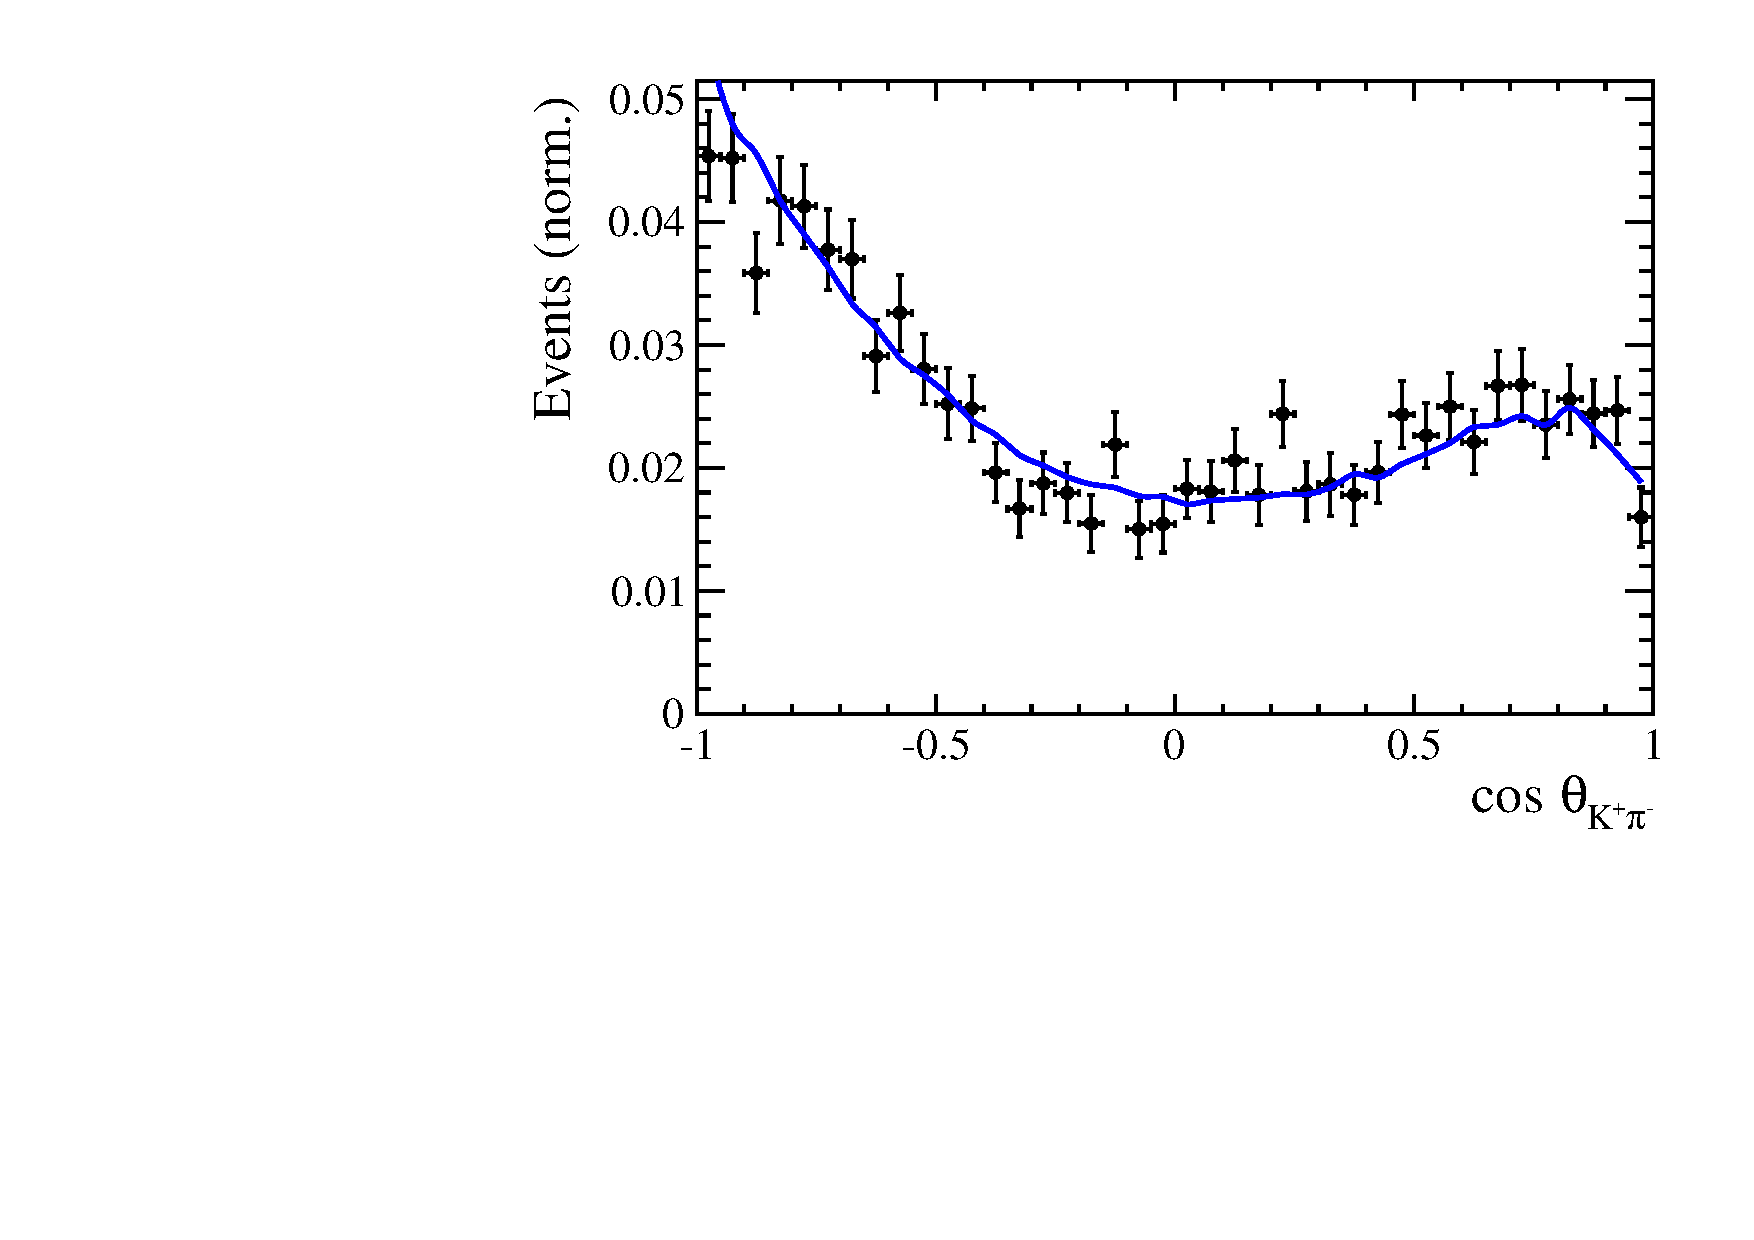
\includegraphics[width=0.3\textwidth, height = !]{figs/fullFit/signal/h_cosTheta_Kpi.pdf} 
		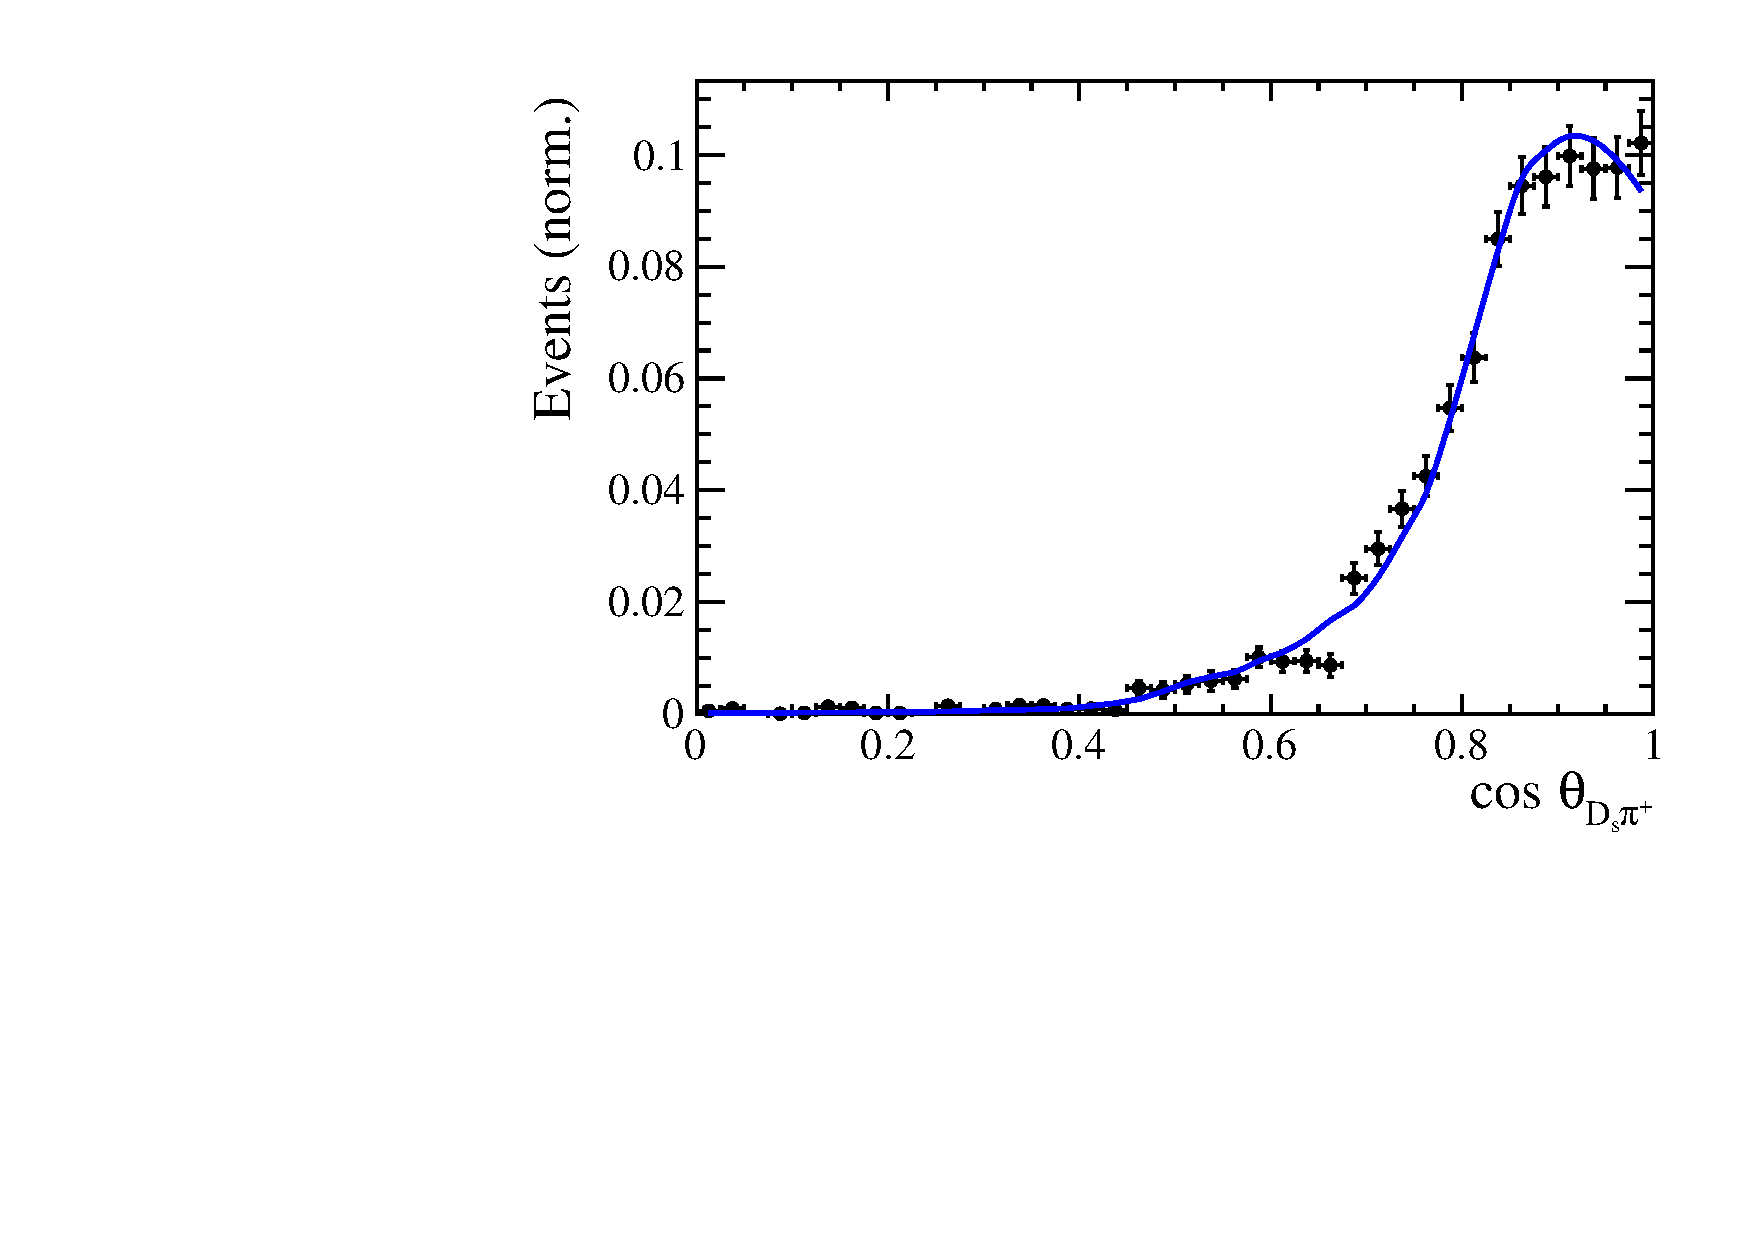
\includegraphics[width=0.3\textwidth, height = !]{figs/fullFit/signal/h_cosTheta_Dspi.pdf} 
		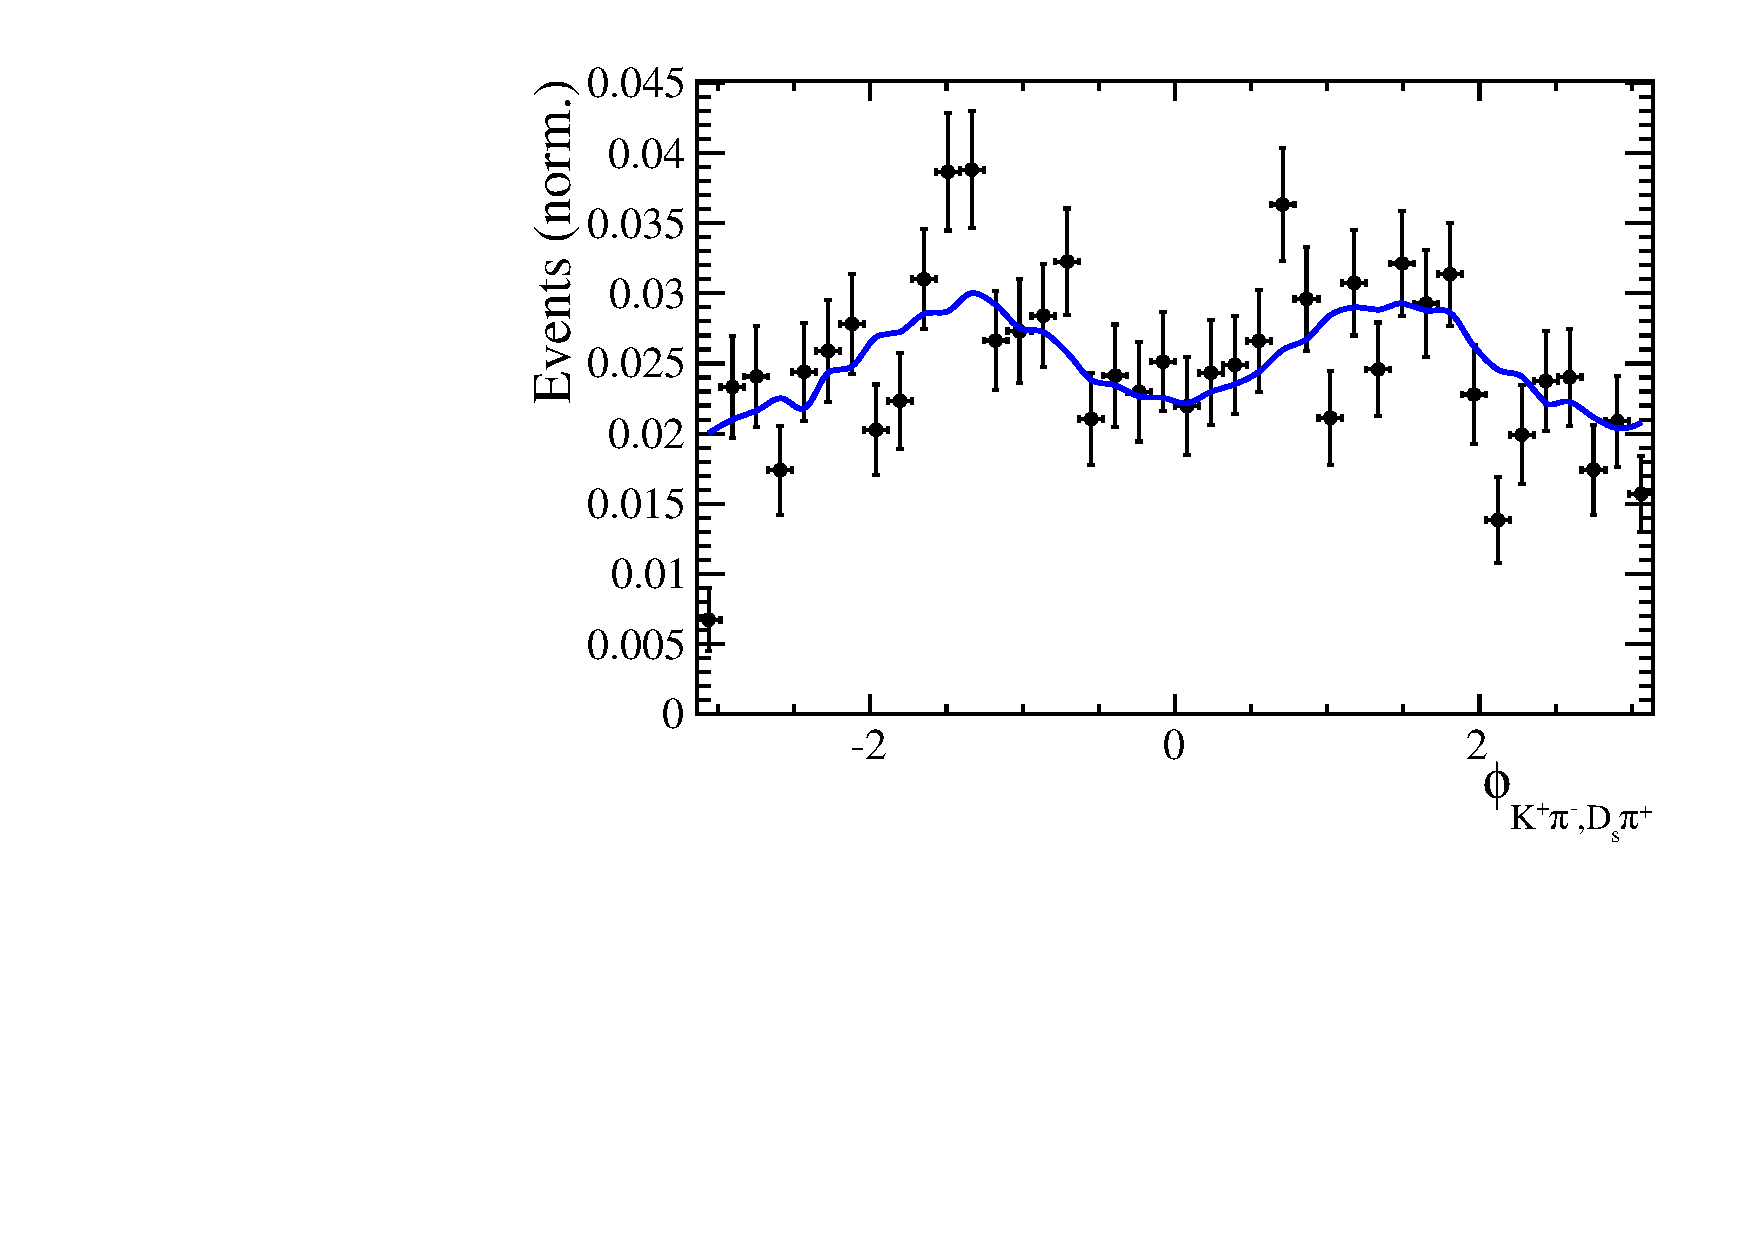
\includegraphics[width=0.3\textwidth, height = !]{figs/fullFit/signal/h_phi_Kpi_Dspi.pdf} 
		
%		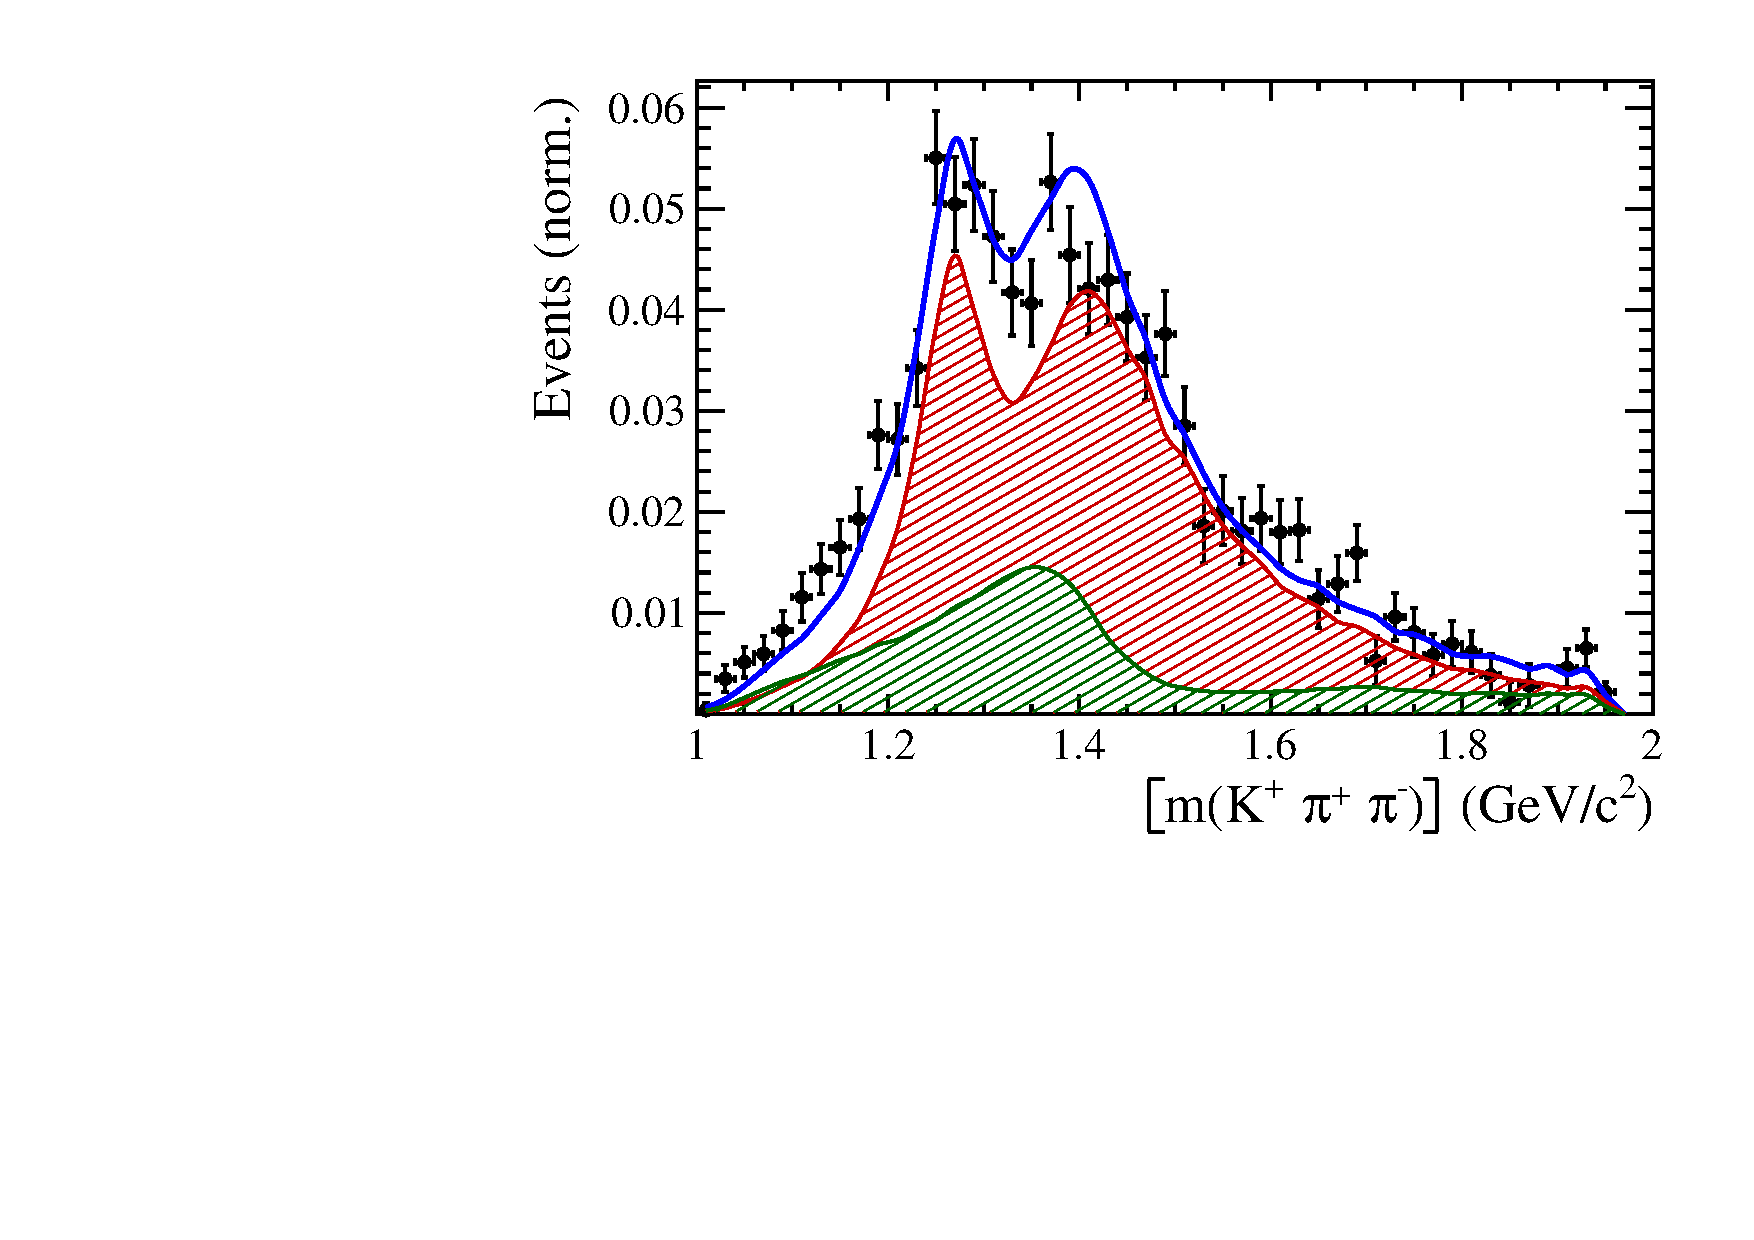
\includegraphics[width=0.3\textwidth, height = !]{figs/fullFit/signal/m_Kpipi_mod.pdf} 
%		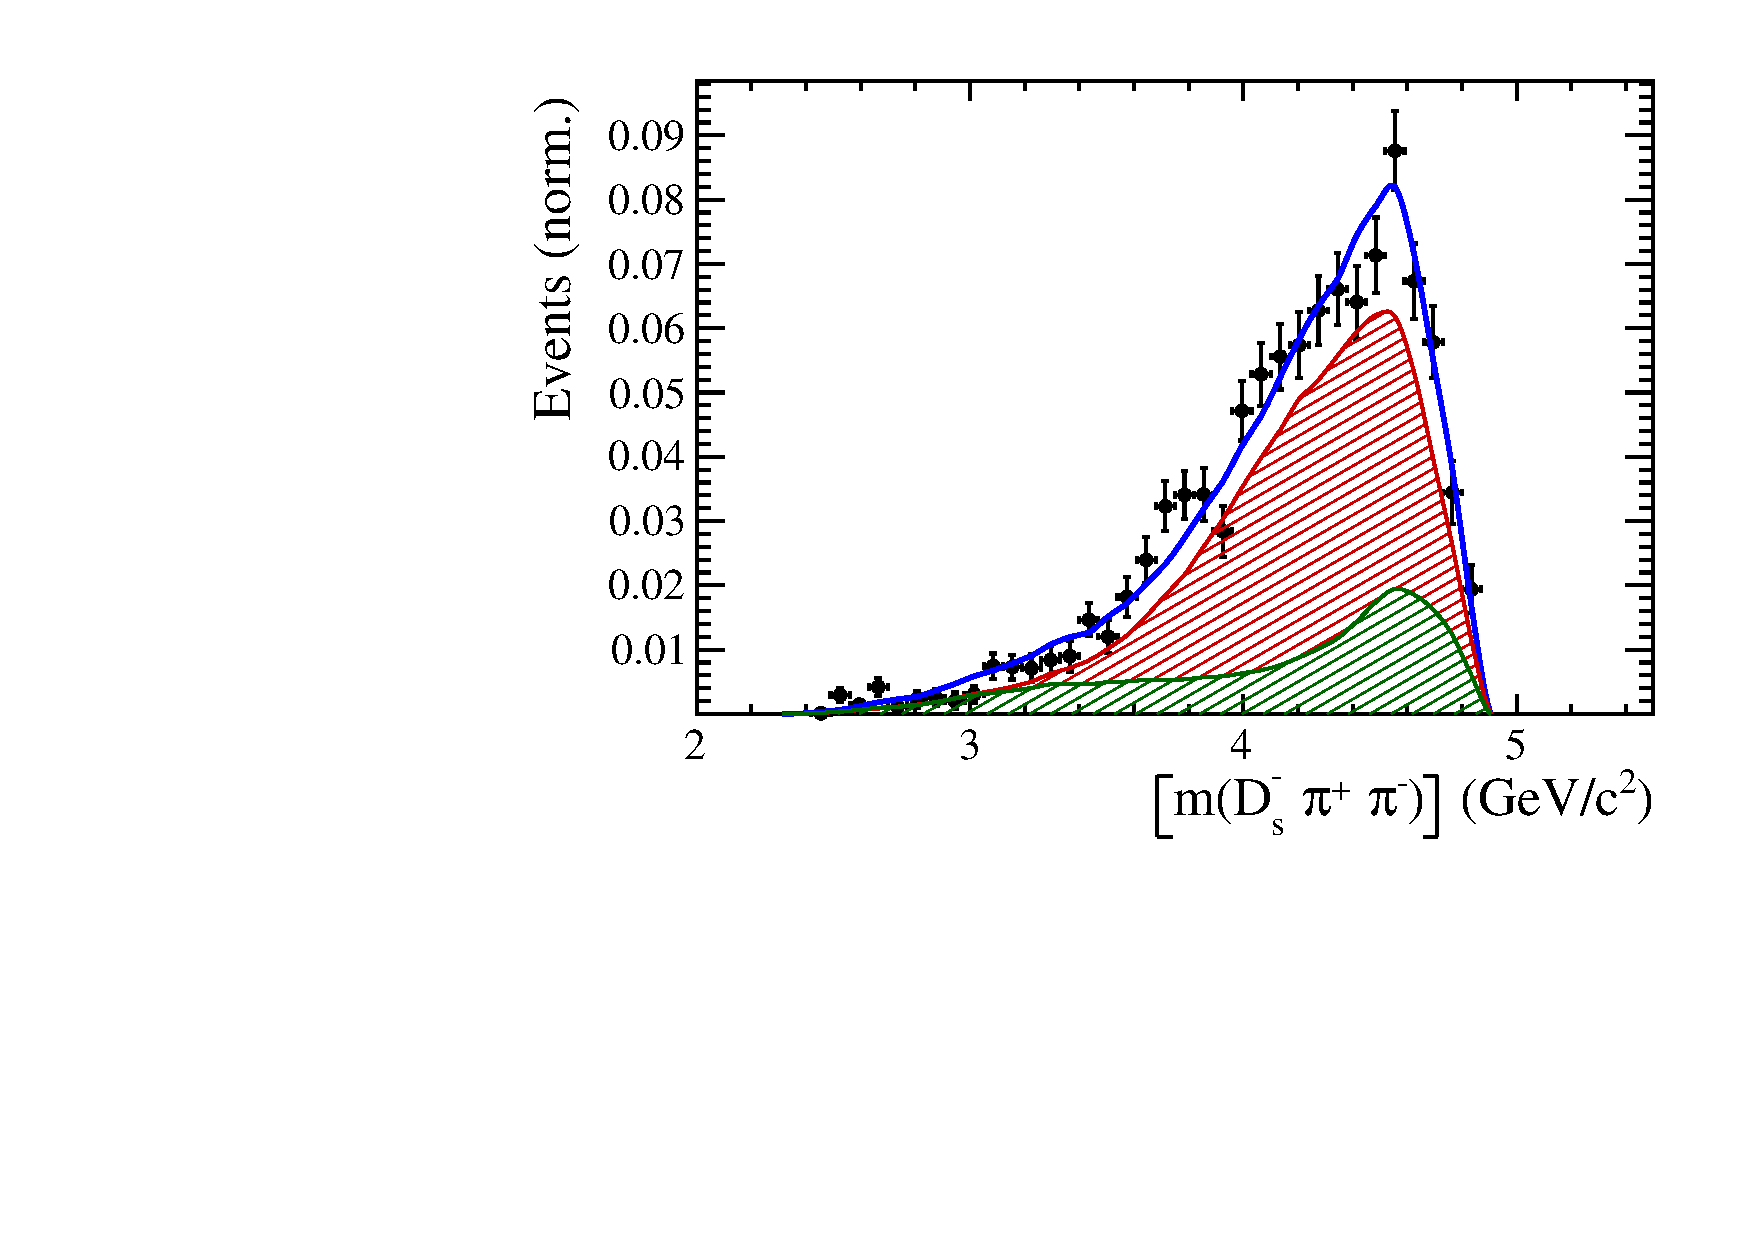
\includegraphics[width=0.3\textwidth, height = !]{figs/fullFit/signal/m_Dspipi_mod.pdf} 

%		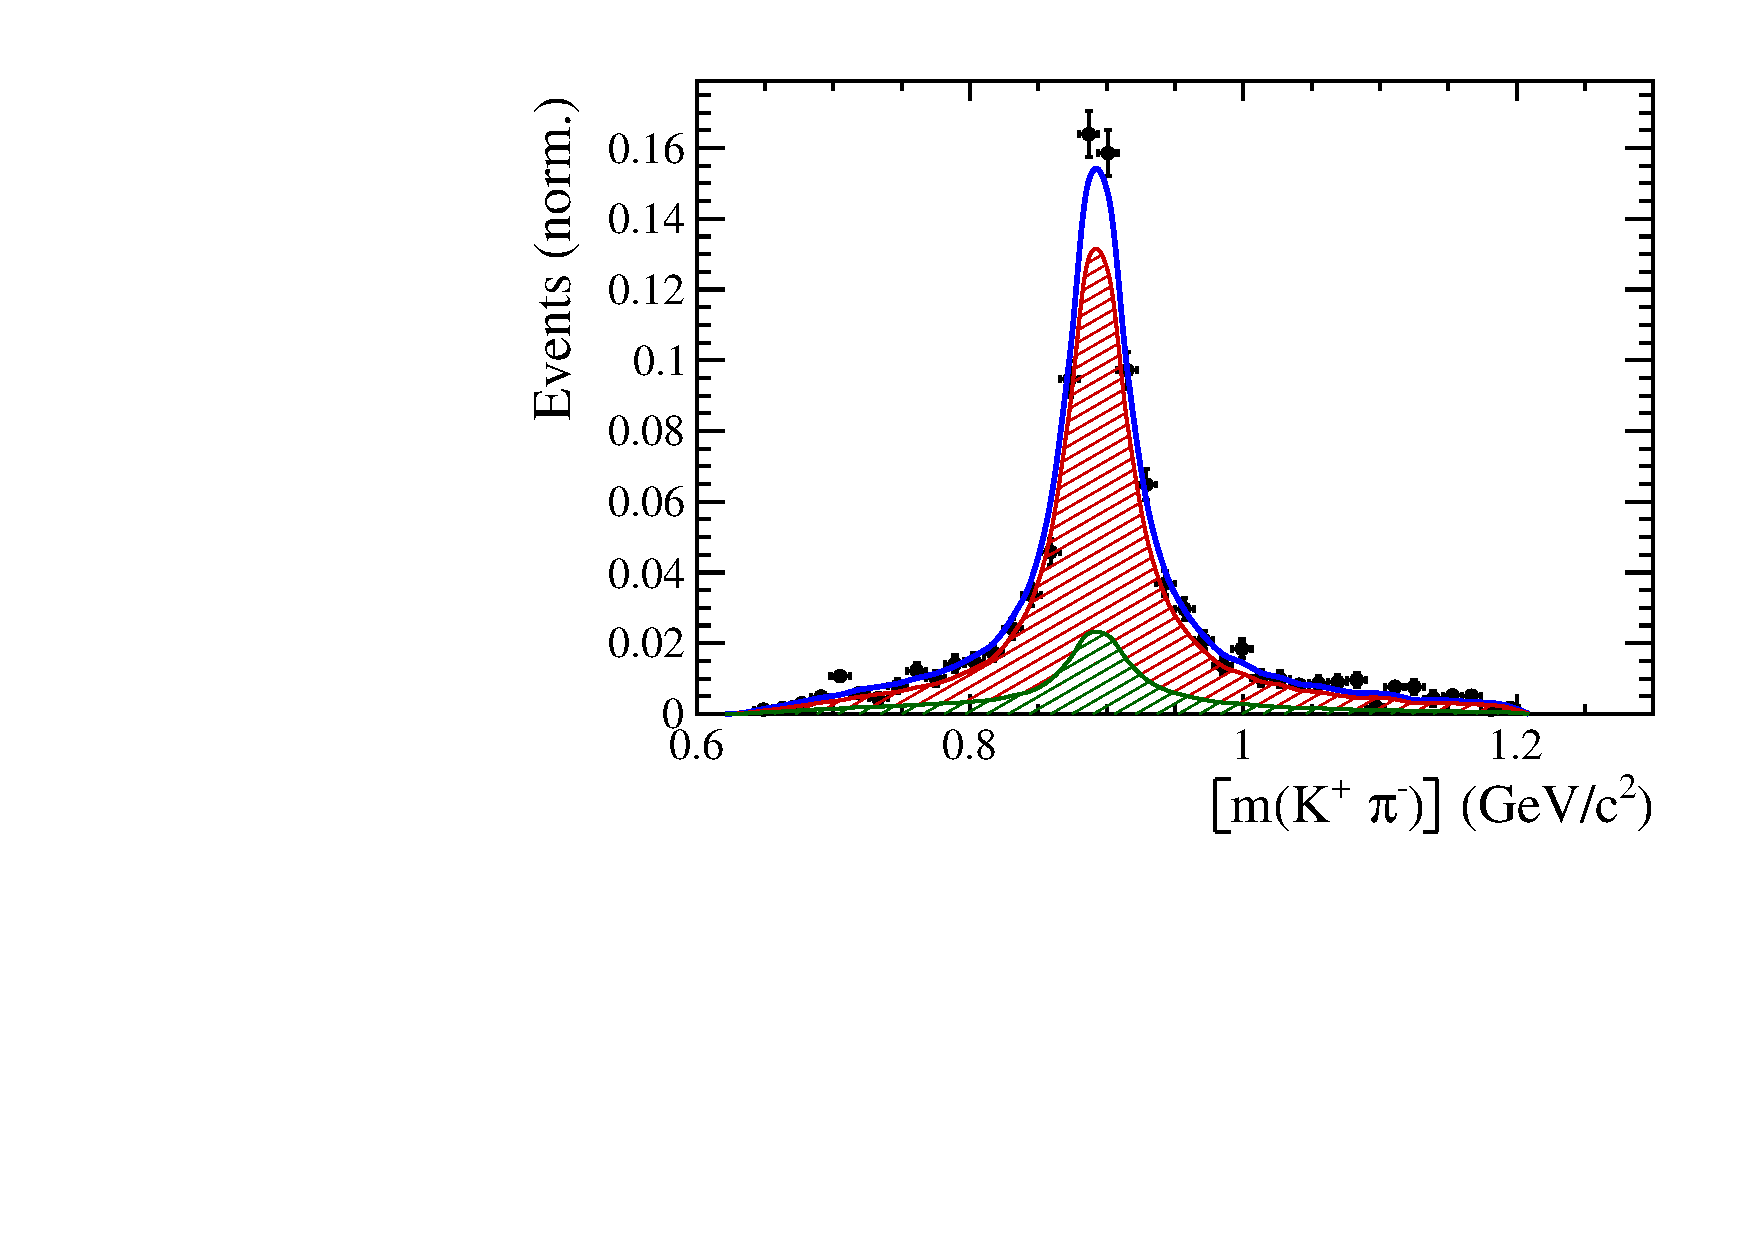
\includegraphics[width=0.3\textwidth, height = !]{figs/fullFit/signal/m_Kpi_mod.pdf} 
%		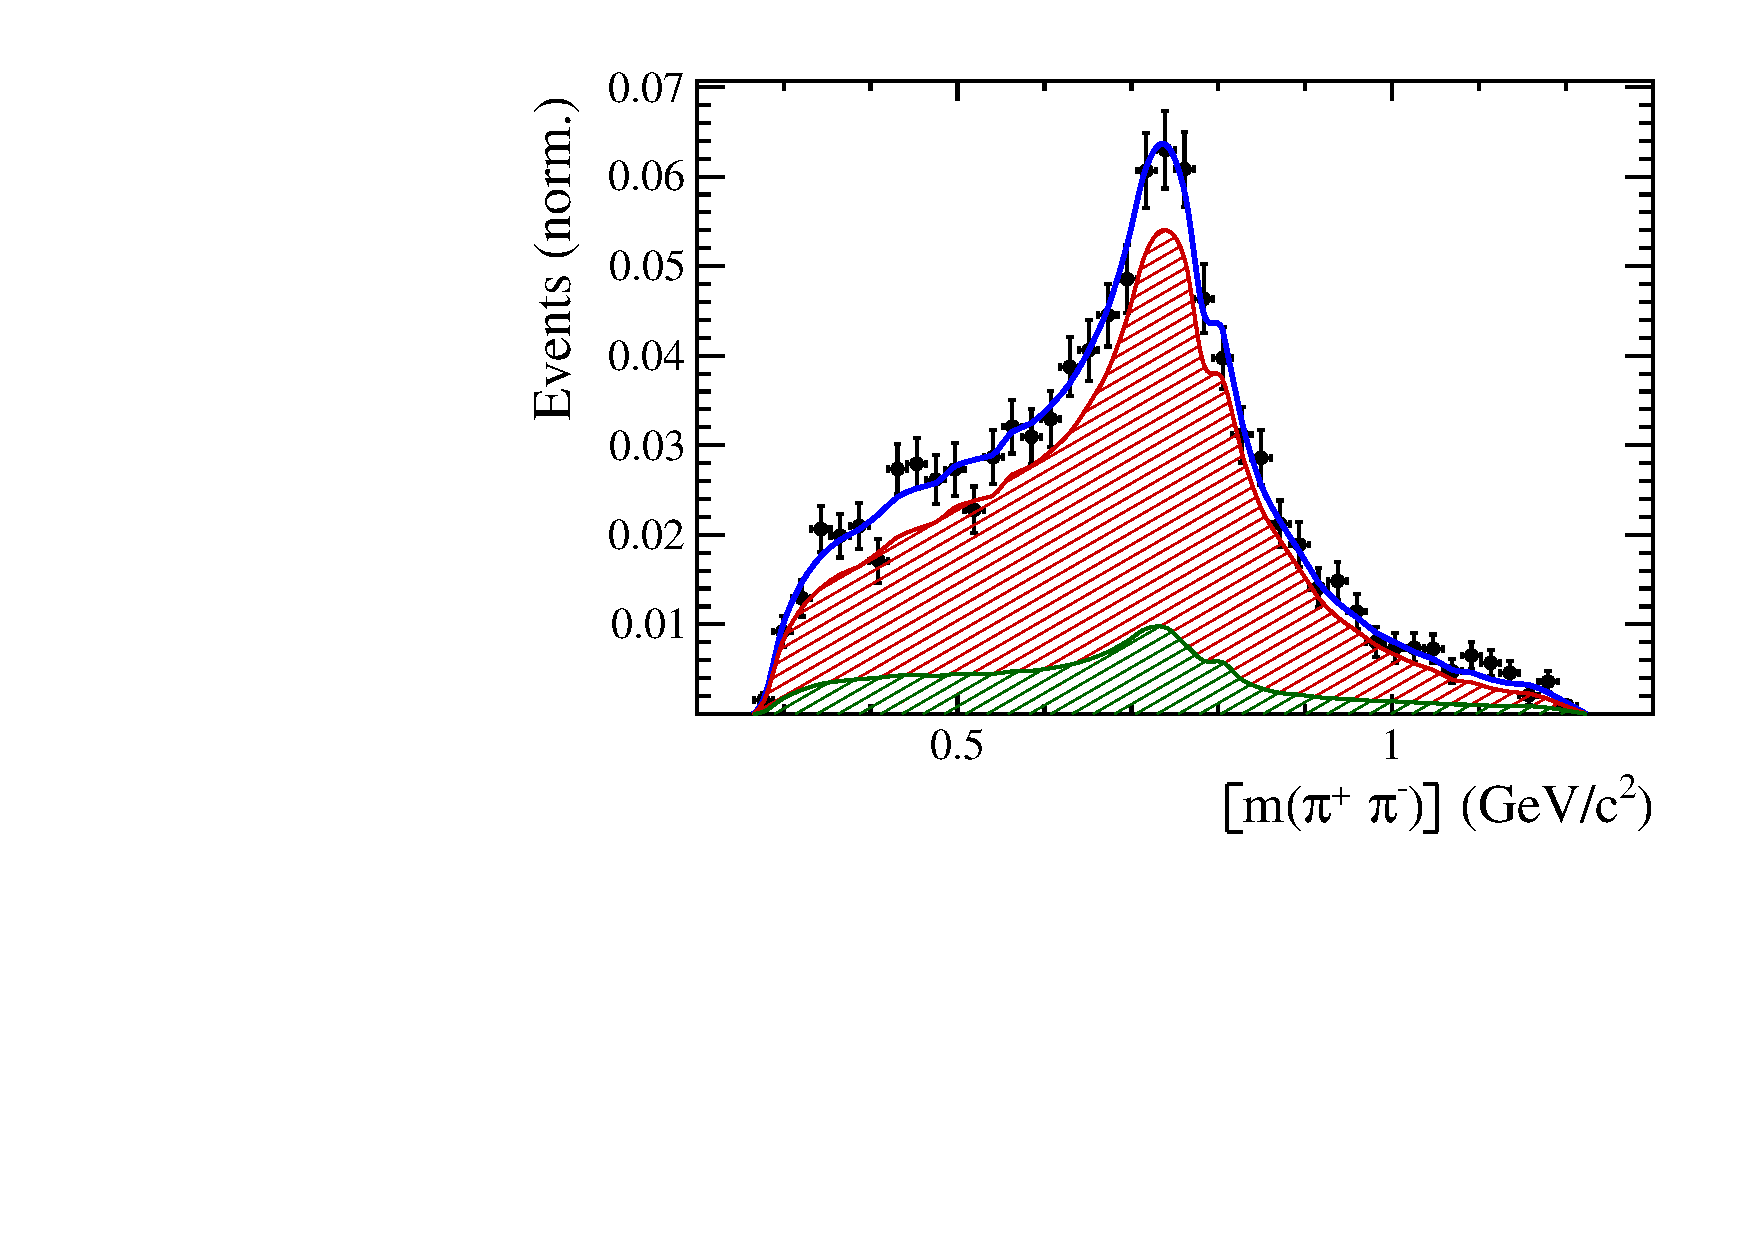
\includegraphics[width=0.3\textwidth, height = !]{figs/fullFit/signal/m_pipi_mod.pdf} 
%		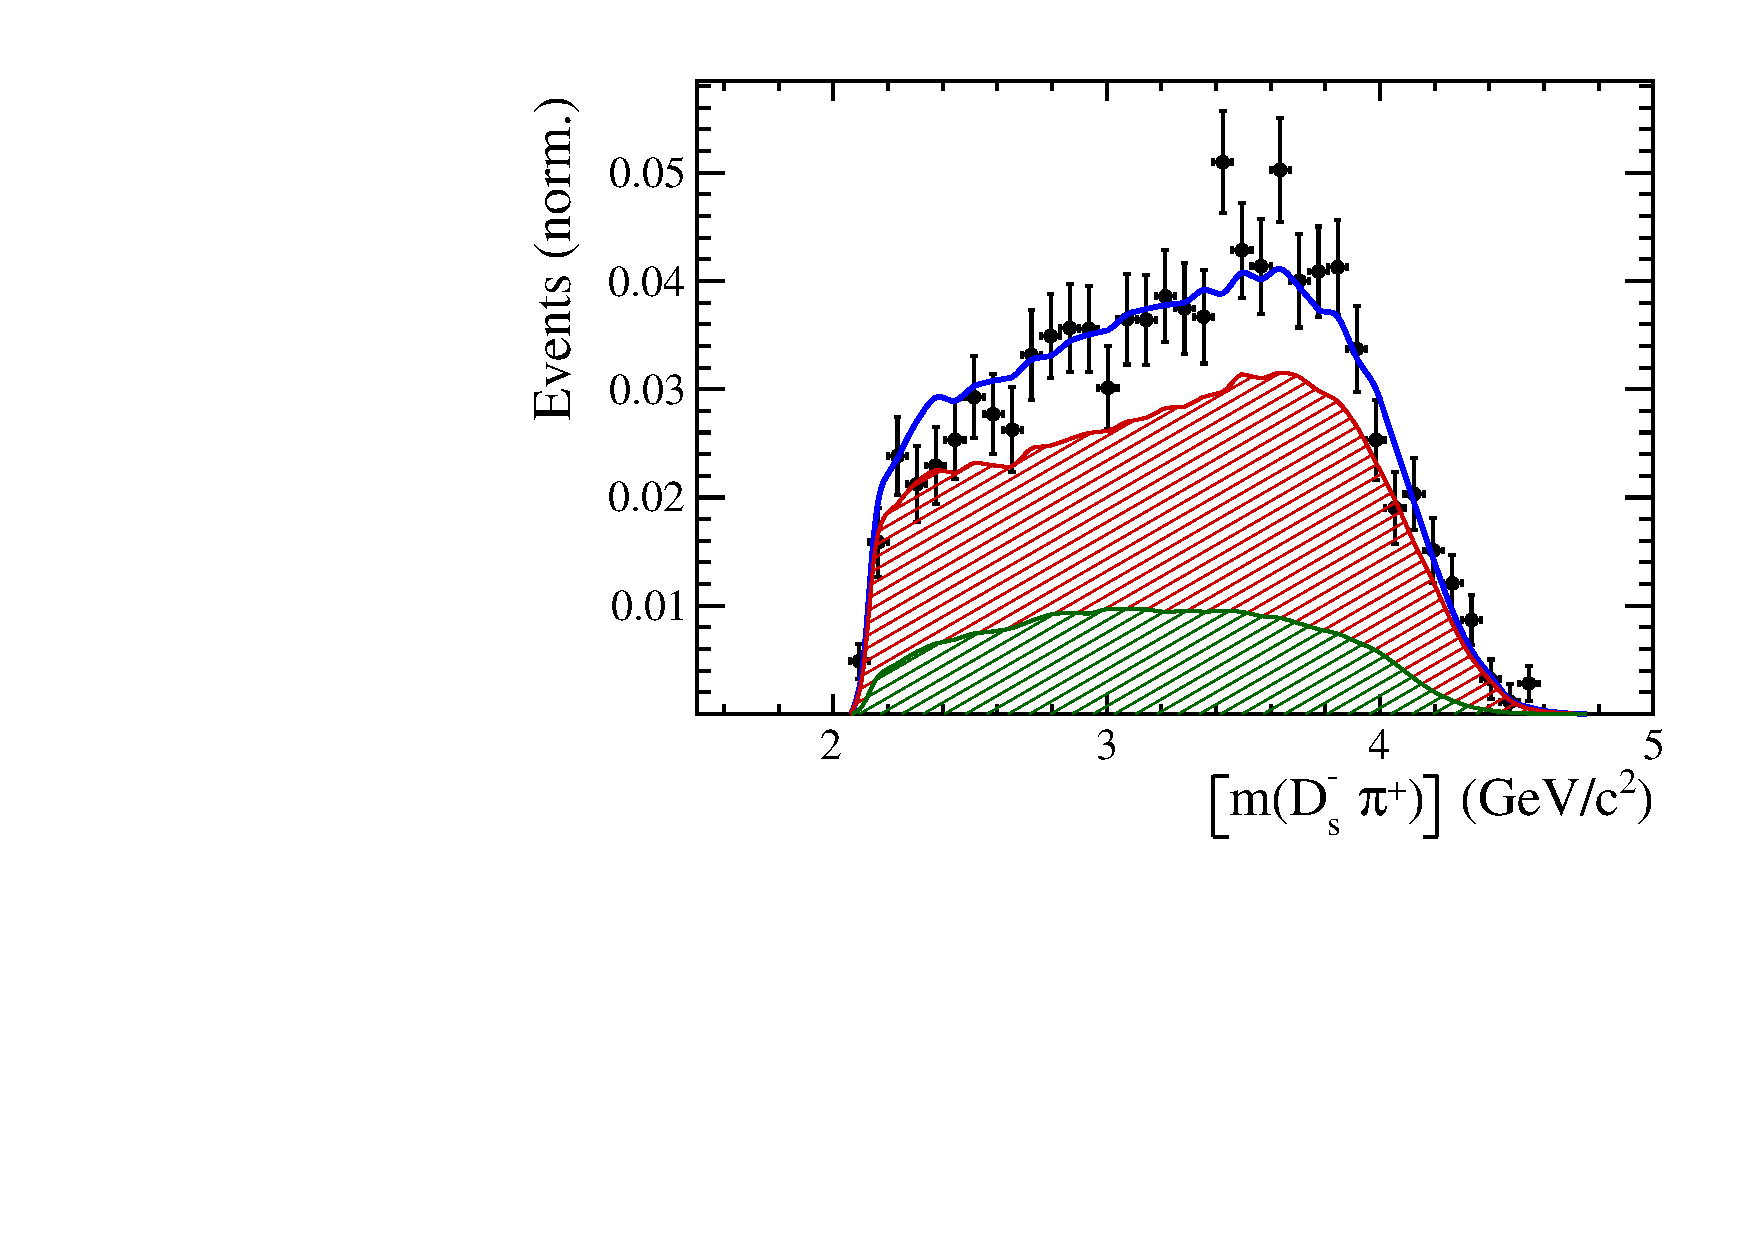
\includegraphics[width=0.3\textwidth, height = !]{figs/fullFit/signal/m_Dspi_mod.pdf} 
%
%		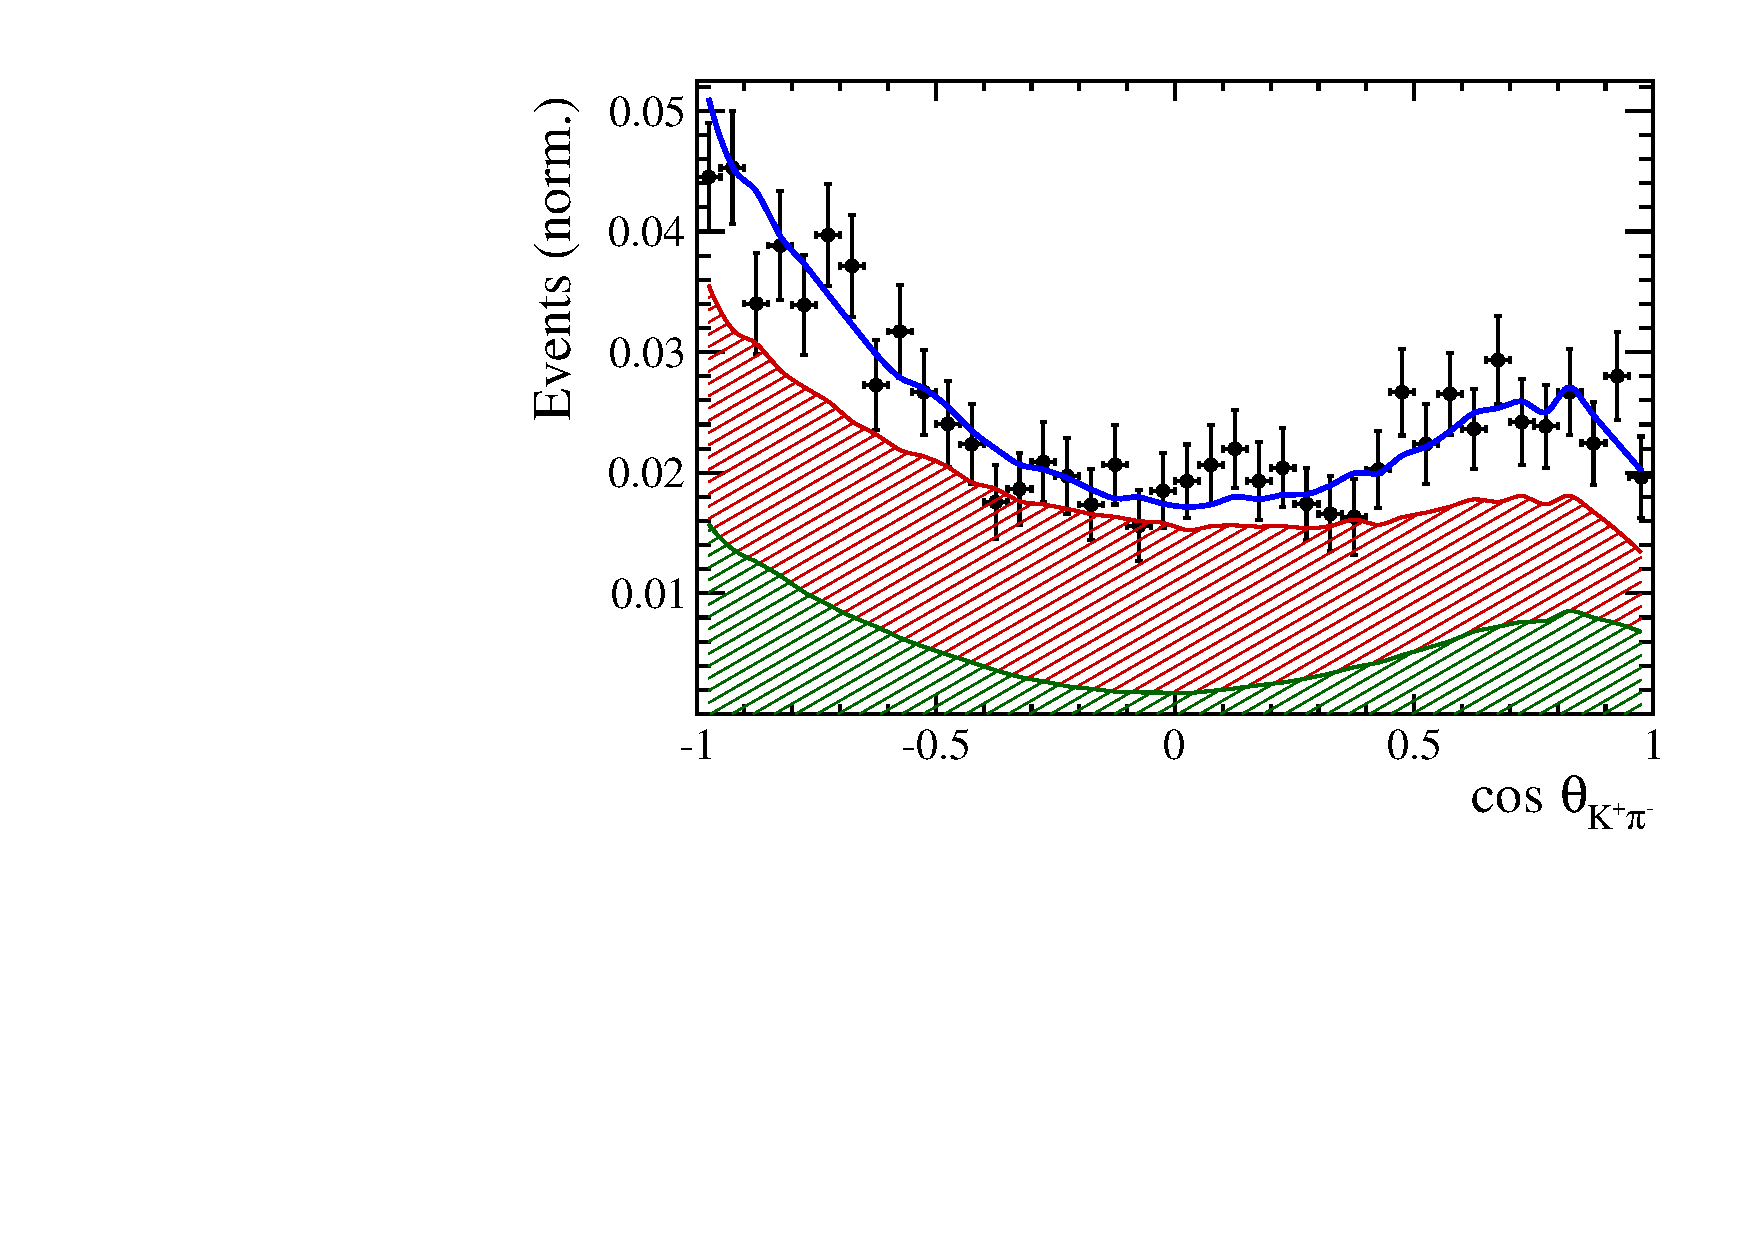
\includegraphics[width=0.3\textwidth, height = !]{figs/fullFit/signal/h_cosTheta_Kpi_mod.pdf} 
%		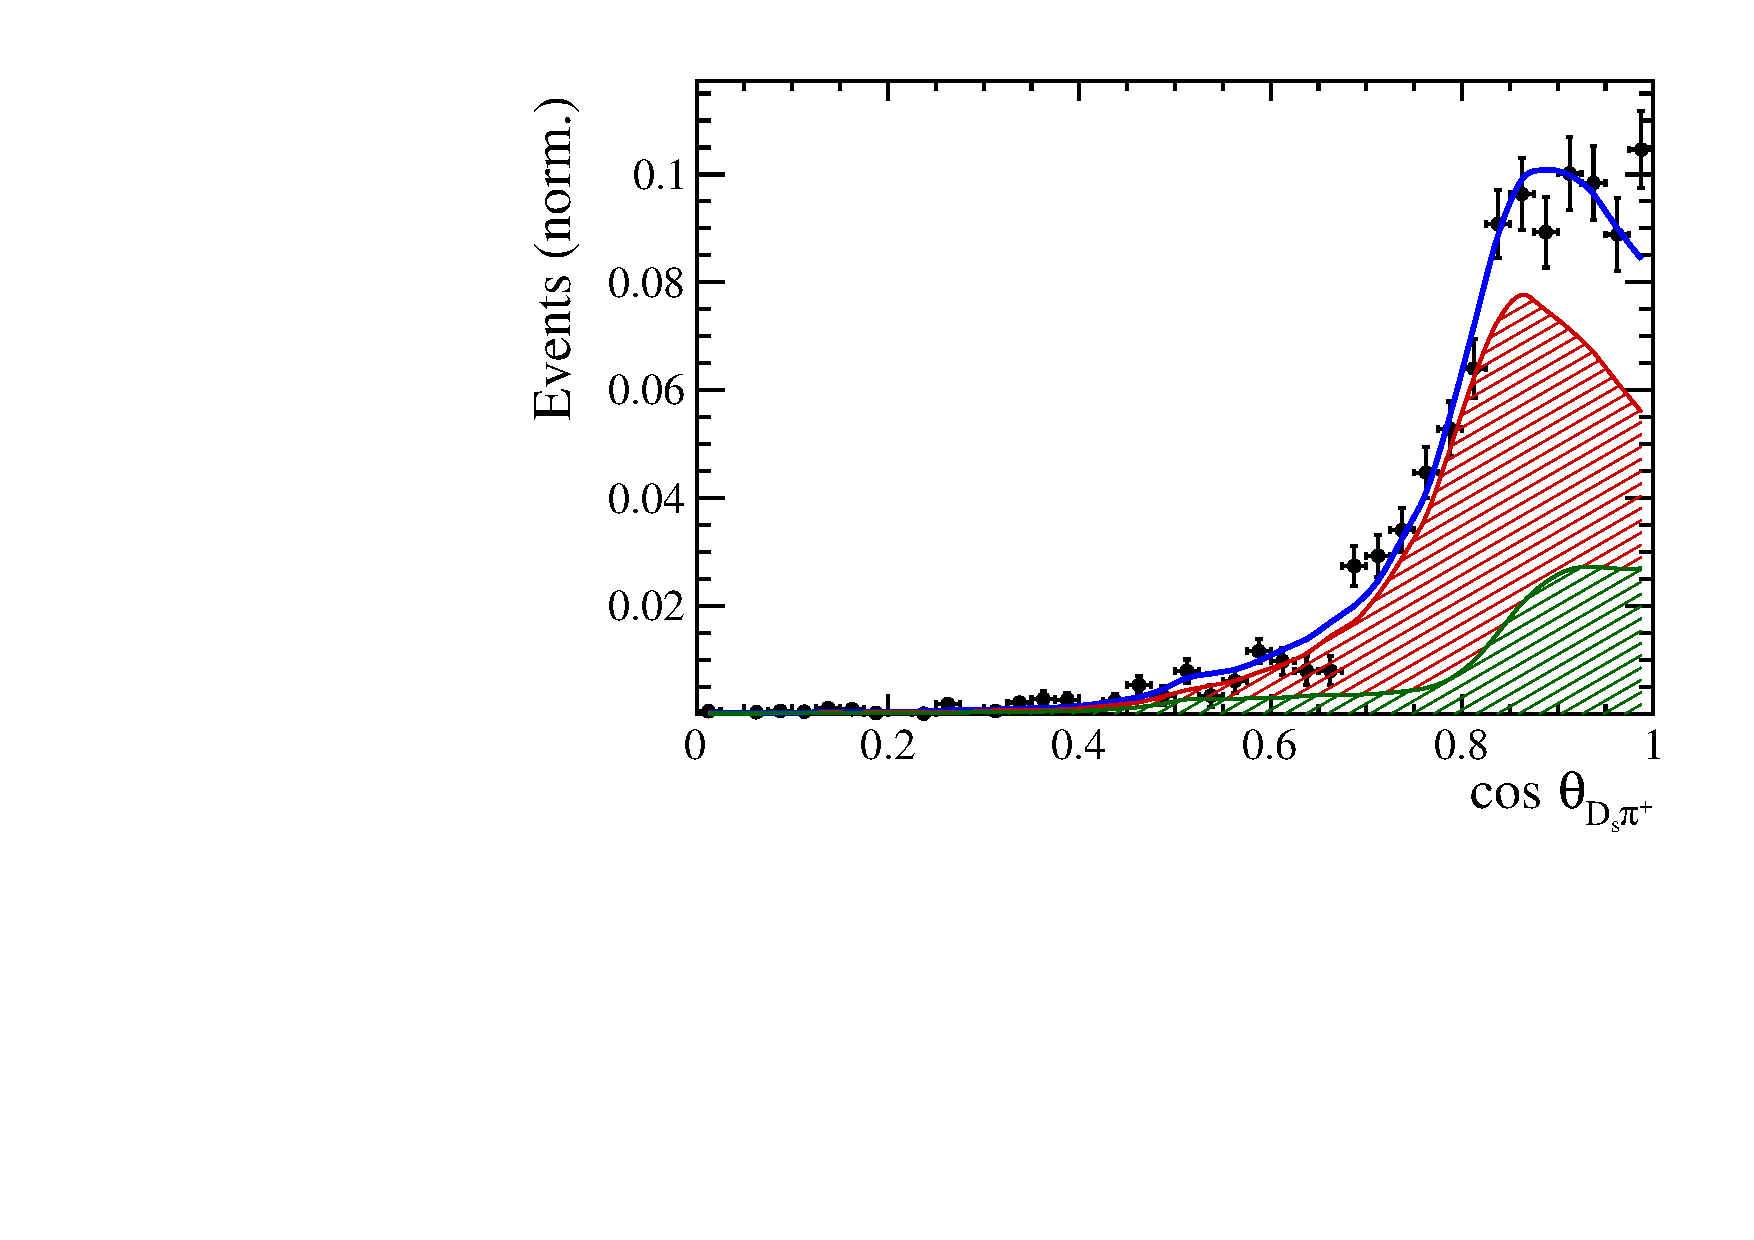
\includegraphics[width=0.3\textwidth, height = !]{figs/fullFit/signal/h_cosTheta_Dspi_mod.pdf} 
%		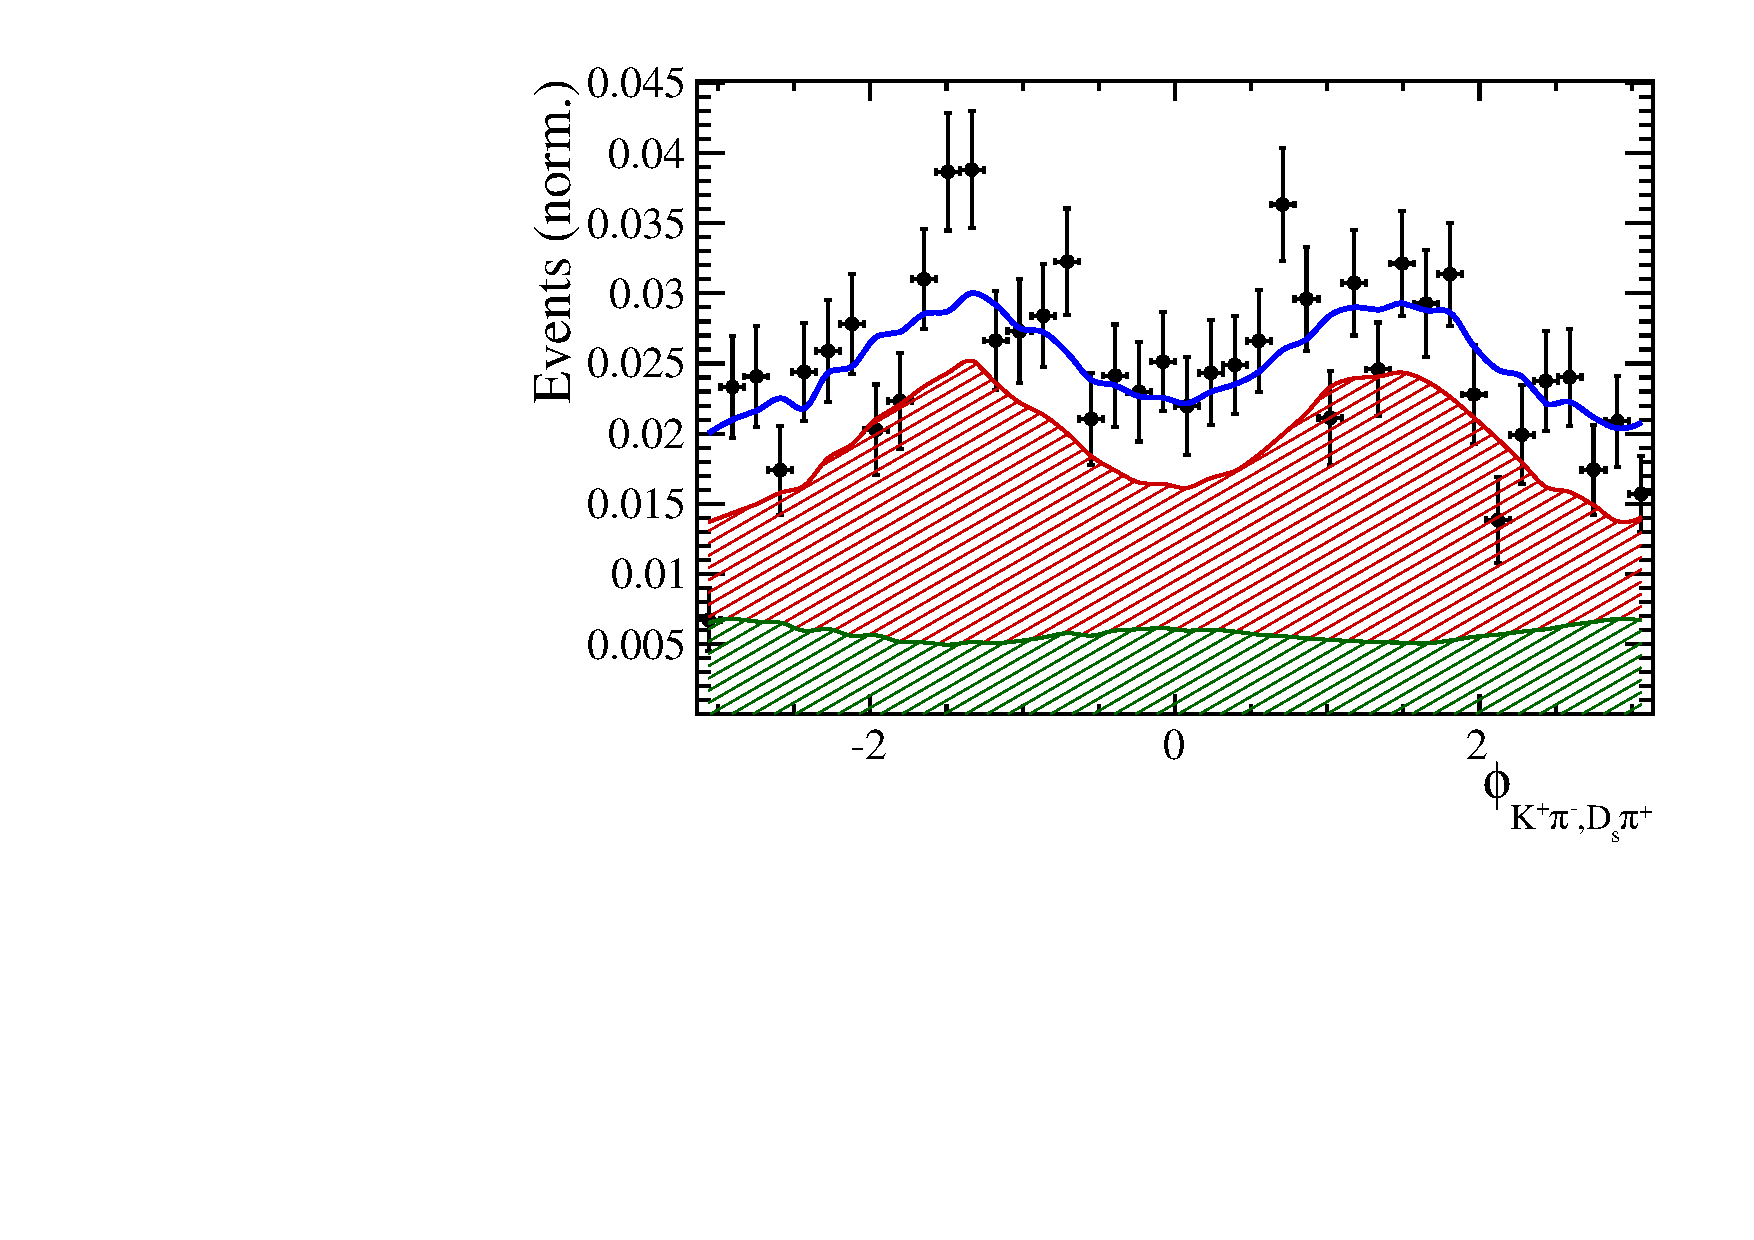
\includegraphics[width=0.3\textwidth, height = !]{figs/fullFit/signal/h_phi_Kpi_Dspi_mod.pdf} 

		\caption{Projections of the full time-dependent amplitude fit.} 		
		\label{fig:fullFit}
\end{figure}	
\begin{table}[h]
\centering
\caption{
Fit fractions of the amplitudes contributing to $b \to c$ and $b \to u$ decays.
}
%\resizebox{\linewidth}{!}{
	\renewcommand{\arraystretch}{1.5}
	\begin{tabular}{l r r } 
\hline
\hline
\multicolumn{1}{c}{Decay Channel} & \multicolumn{1}{c}{$F_{b \to c} [\%]$} & \multicolumn{1}{c}{$F_{b \to u} [\%]$}  \\ 
\hline
$B_s \to D_s \, ( K_1(1270) \to K^{*}(892) \, \pi )$ & 13.1 $\pm$ 2.4 $\pm$ 2.7 $\pm$ 3.6 & 4.5 $\pm$ 2.2 $\pm$ 2.9 $\pm$ 5.0 \\ 
$B_s \to D_s \, ( K_1(1270) \to K \, \rho(770) )$ & 15.6 $\pm$ 1.4 $\pm$ 1.8 $\pm$ 2.6 & 5.3 $\pm$ 2.2 $\pm$ 3.5 $\pm$ 6.4 \\ 
$B_s \to D_s \, ( K_1(1270) \to K^{*}_{0}(1430) \, \pi )$ & 3.2 $\pm$ 0.5 $\pm$ 1.0 $\pm$ 0.5 & 1.1 $\pm$ 0.5 $\pm$ 0.6 $\pm$ 1.4 \\ 
$B_s \to D_s \, ( K_1(1400) \to K^{*}(892) \, \pi )$ & 62.0 $\pm$ 5.1 $\pm$ 7.4 $\pm$ 12.9 & 17.9 $\pm$ 5.2 $\pm$ 8.3 $\pm$ 8.5 \\ 
$B_s \to D_s \, ( K^{*}(1410) \to K^{*}(892) \, \pi )$ & 13.3 $\pm$ 0.8 $\pm$ 1.5 $\pm$ 3.1 & 12.3 $\pm$ 2.0 $\pm$ 2.6 $\pm$ 4.9 \\ 
$B_s \to D_s \, ( K^{*}(1410) \to K \, \rho(770) )$ & 5.8 $\pm$ 0.4 $\pm$ 0.6 $\pm$ 0.7 & 5.4 $\pm$ 1.0 $\pm$ 1.2 $\pm$ 2.1 \\ 
$B_s \to D_s \, ( K(1460) \to K^{*}(892) \, \pi )$ &  & 12.0 $\pm$ 2.5 $\pm$ 2.9 $\pm$ 3.2 \\ 
$B_s \to ( D_s \, \pi)_{P} \, \, K^{*}(892)$ & 9.8 $\pm$ 1.6 $\pm$ 1.8 $\pm$ 4.3 & 29.4 $\pm$ 5.6 $\pm$ 6.4 $\pm$ 14.8 \\ 
$B_s \to ( D_s \, K)_{P} \, \, \rho(770)$ & 0.9 $\pm$ 0.4 $\pm$ 0.5 $\pm$ 1.0 &  \\ 
\hline
$\text{Sum}$ & 123.8 $\pm$ 6.4 $\pm$ 6.9 $\pm$ 19.4 & 87.8 $\pm$ 7.0 $\pm$ 10.0 $\pm$ 20.1 \\ 
\hline
\hline
\end{tabular}

%}
\label{tab:fullFractions}
\end{table}


